% Options for packages loaded elsewhere
\PassOptionsToPackage{unicode}{hyperref}
\PassOptionsToPackage{hyphens}{url}
%
\documentclass[
]{article}
\usepackage{amsmath,amssymb}
\usepackage{lmodern}
\usepackage{iftex}
\ifPDFTeX
  \usepackage[T1]{fontenc}
  \usepackage[utf8]{inputenc}
  \usepackage{textcomp} % provide euro and other symbols
\else % if luatex or xetex
  \usepackage{unicode-math}
  \defaultfontfeatures{Scale=MatchLowercase}
  \defaultfontfeatures[\rmfamily]{Ligatures=TeX,Scale=1}
\fi
% Use upquote if available, for straight quotes in verbatim environments
\IfFileExists{upquote.sty}{\usepackage{upquote}}{}
\IfFileExists{microtype.sty}{% use microtype if available
  \usepackage[]{microtype}
  \UseMicrotypeSet[protrusion]{basicmath} % disable protrusion for tt fonts
}{}
\makeatletter
\@ifundefined{KOMAClassName}{% if non-KOMA class
  \IfFileExists{parskip.sty}{%
    \usepackage{parskip}
  }{% else
    \setlength{\parindent}{0pt}
    \setlength{\parskip}{6pt plus 2pt minus 1pt}}
}{% if KOMA class
  \KOMAoptions{parskip=half}}
\makeatother
\usepackage{xcolor}
\usepackage[left=3cm,right=3cm,top=2cm,bottom=2cm]{geometry}
\usepackage{color}
\usepackage{fancyvrb}
\newcommand{\VerbBar}{|}
\newcommand{\VERB}{\Verb[commandchars=\\\{\}]}
\DefineVerbatimEnvironment{Highlighting}{Verbatim}{commandchars=\\\{\}}
% Add ',fontsize=\small' for more characters per line
\usepackage{framed}
\definecolor{shadecolor}{RGB}{248,248,248}
\newenvironment{Shaded}{\begin{snugshade}}{\end{snugshade}}
\newcommand{\AlertTok}[1]{\textcolor[rgb]{0.94,0.16,0.16}{#1}}
\newcommand{\AnnotationTok}[1]{\textcolor[rgb]{0.56,0.35,0.01}{\textbf{\textit{#1}}}}
\newcommand{\AttributeTok}[1]{\textcolor[rgb]{0.77,0.63,0.00}{#1}}
\newcommand{\BaseNTok}[1]{\textcolor[rgb]{0.00,0.00,0.81}{#1}}
\newcommand{\BuiltInTok}[1]{#1}
\newcommand{\CharTok}[1]{\textcolor[rgb]{0.31,0.60,0.02}{#1}}
\newcommand{\CommentTok}[1]{\textcolor[rgb]{0.56,0.35,0.01}{\textit{#1}}}
\newcommand{\CommentVarTok}[1]{\textcolor[rgb]{0.56,0.35,0.01}{\textbf{\textit{#1}}}}
\newcommand{\ConstantTok}[1]{\textcolor[rgb]{0.00,0.00,0.00}{#1}}
\newcommand{\ControlFlowTok}[1]{\textcolor[rgb]{0.13,0.29,0.53}{\textbf{#1}}}
\newcommand{\DataTypeTok}[1]{\textcolor[rgb]{0.13,0.29,0.53}{#1}}
\newcommand{\DecValTok}[1]{\textcolor[rgb]{0.00,0.00,0.81}{#1}}
\newcommand{\DocumentationTok}[1]{\textcolor[rgb]{0.56,0.35,0.01}{\textbf{\textit{#1}}}}
\newcommand{\ErrorTok}[1]{\textcolor[rgb]{0.64,0.00,0.00}{\textbf{#1}}}
\newcommand{\ExtensionTok}[1]{#1}
\newcommand{\FloatTok}[1]{\textcolor[rgb]{0.00,0.00,0.81}{#1}}
\newcommand{\FunctionTok}[1]{\textcolor[rgb]{0.00,0.00,0.00}{#1}}
\newcommand{\ImportTok}[1]{#1}
\newcommand{\InformationTok}[1]{\textcolor[rgb]{0.56,0.35,0.01}{\textbf{\textit{#1}}}}
\newcommand{\KeywordTok}[1]{\textcolor[rgb]{0.13,0.29,0.53}{\textbf{#1}}}
\newcommand{\NormalTok}[1]{#1}
\newcommand{\OperatorTok}[1]{\textcolor[rgb]{0.81,0.36,0.00}{\textbf{#1}}}
\newcommand{\OtherTok}[1]{\textcolor[rgb]{0.56,0.35,0.01}{#1}}
\newcommand{\PreprocessorTok}[1]{\textcolor[rgb]{0.56,0.35,0.01}{\textit{#1}}}
\newcommand{\RegionMarkerTok}[1]{#1}
\newcommand{\SpecialCharTok}[1]{\textcolor[rgb]{0.00,0.00,0.00}{#1}}
\newcommand{\SpecialStringTok}[1]{\textcolor[rgb]{0.31,0.60,0.02}{#1}}
\newcommand{\StringTok}[1]{\textcolor[rgb]{0.31,0.60,0.02}{#1}}
\newcommand{\VariableTok}[1]{\textcolor[rgb]{0.00,0.00,0.00}{#1}}
\newcommand{\VerbatimStringTok}[1]{\textcolor[rgb]{0.31,0.60,0.02}{#1}}
\newcommand{\WarningTok}[1]{\textcolor[rgb]{0.56,0.35,0.01}{\textbf{\textit{#1}}}}
\usepackage{graphicx}
\makeatletter
\def\maxwidth{\ifdim\Gin@nat@width>\linewidth\linewidth\else\Gin@nat@width\fi}
\def\maxheight{\ifdim\Gin@nat@height>\textheight\textheight\else\Gin@nat@height\fi}
\makeatother
% Scale images if necessary, so that they will not overflow the page
% margins by default, and it is still possible to overwrite the defaults
% using explicit options in \includegraphics[width, height, ...]{}
\setkeys{Gin}{width=\maxwidth,height=\maxheight,keepaspectratio}
% Set default figure placement to htbp
\makeatletter
\def\fps@figure{htbp}
\makeatother
\setlength{\emergencystretch}{3em} % prevent overfull lines
\providecommand{\tightlist}{%
  \setlength{\itemsep}{0pt}\setlength{\parskip}{0pt}}
\setcounter{secnumdepth}{5}
\usepackage{booktabs}
\usepackage{longtable}
\usepackage{array}
\usepackage{multirow}
\usepackage{wrapfig}
\usepackage{float}
\usepackage{colortbl}
\usepackage{pdflscape}
\usepackage{tabu}
\usepackage{threeparttable}
\usepackage{threeparttablex}
\usepackage[normalem]{ulem}
\usepackage{makecell}
\usepackage{xcolor}
\ifLuaTeX
  \usepackage{selnolig}  % disable illegal ligatures
\fi
\IfFileExists{bookmark.sty}{\usepackage{bookmark}}{\usepackage{hyperref}}
\IfFileExists{xurl.sty}{\usepackage{xurl}}{} % add URL line breaks if available
\urlstyle{same} % disable monospaced font for URLs
\hypersetup{
  pdftitle={Will it Rain Tomorrow in Australia?},
  pdfauthor={Sofia Pope Trogu; Fairouz Baz Radwan; Auriane Mahfouz},
  hidelinks,
  pdfcreator={LaTeX via pandoc}}

\title{Will it Rain Tomorrow in Australia?}
\author{Sofia Pope Trogu \and Fairouz Baz Radwan \and Auriane Mahfouz}
\date{17-07-2023}

\begin{document}
\maketitle

{
\setcounter{tocdepth}{2}
\tableofcontents
}
\hypertarget{import-r-libraries}{%
\section{Import R Libraries}\label{import-r-libraries}}

\begin{Shaded}
\begin{Highlighting}[]
\FunctionTok{library}\NormalTok{(corrplot)}
\FunctionTok{library}\NormalTok{(ggplot2)}
\FunctionTok{library}\NormalTok{(caret)}
\FunctionTok{library}\NormalTok{(magrittr)}
\FunctionTok{library}\NormalTok{(gridExtra)  }
\FunctionTok{library}\NormalTok{(scales)}
\FunctionTok{library}\NormalTok{(DMwR2)}
\FunctionTok{library}\NormalTok{(UBL)}
\FunctionTok{library}\NormalTok{(caret)}
\FunctionTok{library}\NormalTok{(MASS)}
\FunctionTok{library}\NormalTok{(ipred)}
\FunctionTok{library}\NormalTok{(rsample)}
\FunctionTok{library}\NormalTok{(mlr)}
\FunctionTok{library}\NormalTok{(knitr)}
\FunctionTok{library}\NormalTok{(glmnet)}
\FunctionTok{library}\NormalTok{(outliers)}
\FunctionTok{library}\NormalTok{(class)}
\FunctionTok{library}\NormalTok{(kableExtra)}
\FunctionTok{library}\NormalTok{(tidyverse)}
\FunctionTok{library}\NormalTok{(pROC)}
\FunctionTok{library}\NormalTok{(dplyr)}
\end{Highlighting}
\end{Shaded}

\hypertarget{data-preparation}{%
\section{Data Preparation}\label{data-preparation}}

\hypertarget{download-the-rain-dataset}{%
\subsection{Download the Rain Dataset}\label{download-the-rain-dataset}}

We downloaded the Rain Australia dataset as a CSV from the following
link:
\url{https://www.kaggle.com/datasets/jsphyg/weather-dataset-rattle-package/code?datasetId=6012\&searchQuery=visual}.
The dataset is originally composed of 23 columns and 145,460 examples.
The aim of the data is to use available information about today's
weather, i.e. Temperature, Humidity, Pressure, to predict whether it
will rain tomorrow. Therefore, we originally start with 22 features and
1 target variable, RainTomorrow with binary classification (Yes=1,
No=0).

\begin{Shaded}
\begin{Highlighting}[]
\NormalTok{file\_path }\OtherTok{\textless{}{-}} \StringTok{"/Users/Sofia/Desktop/Rain\_Australia/weatherAUS.csv"}
\NormalTok{rain }\OtherTok{\textless{}{-}} \FunctionTok{read.csv}\NormalTok{(file\_path)}
\FunctionTok{head}\NormalTok{(rain)}
\end{Highlighting}
\end{Shaded}

\begin{verbatim}
##         Date Location MinTemp MaxTemp Rainfall Evaporation Sunshine WindGustDir
## 1 2008-12-01   Albury    13.4    22.9      0.6          NA       NA           W
## 2 2008-12-02   Albury     7.4    25.1      0.0          NA       NA         WNW
## 3 2008-12-03   Albury    12.9    25.7      0.0          NA       NA         WSW
## 4 2008-12-04   Albury     9.2    28.0      0.0          NA       NA          NE
## 5 2008-12-05   Albury    17.5    32.3      1.0          NA       NA           W
## 6 2008-12-06   Albury    14.6    29.7      0.2          NA       NA         WNW
##   WindGustSpeed WindDir9am WindDir3pm WindSpeed9am WindSpeed3pm Humidity9am
## 1            44          W        WNW           20           24          71
## 2            44        NNW        WSW            4           22          44
## 3            46          W        WSW           19           26          38
## 4            24         SE          E           11            9          45
## 5            41        ENE         NW            7           20          82
## 6            56          W          W           19           24          55
##   Humidity3pm Pressure9am Pressure3pm Cloud9am Cloud3pm Temp9am Temp3pm
## 1          22      1007.7      1007.1        8       NA    16.9    21.8
## 2          25      1010.6      1007.8       NA       NA    17.2    24.3
## 3          30      1007.6      1008.7       NA        2    21.0    23.2
## 4          16      1017.6      1012.8       NA       NA    18.1    26.5
## 5          33      1010.8      1006.0        7        8    17.8    29.7
## 6          23      1009.2      1005.4       NA       NA    20.6    28.9
##   RainToday RainTomorrow
## 1        No           No
## 2        No           No
## 3        No           No
## 4        No           No
## 5        No           No
## 6        No           No
\end{verbatim}

\begin{Shaded}
\begin{Highlighting}[]
\FunctionTok{summary}\NormalTok{(rain)}
\end{Highlighting}
\end{Shaded}

\begin{verbatim}
##      Date             Location            MinTemp         MaxTemp     
##  Length:145460      Length:145460      Min.   :-8.50   Min.   :-4.80  
##  Class :character   Class :character   1st Qu.: 7.60   1st Qu.:17.90  
##  Mode  :character   Mode  :character   Median :12.00   Median :22.60  
##                                        Mean   :12.19   Mean   :23.22  
##                                        3rd Qu.:16.90   3rd Qu.:28.20  
##                                        Max.   :33.90   Max.   :48.10  
##                                        NA's   :1485    NA's   :1261   
##     Rainfall        Evaporation        Sunshine     WindGustDir       
##  Min.   :  0.000   Min.   :  0.00   Min.   : 0.00   Length:145460     
##  1st Qu.:  0.000   1st Qu.:  2.60   1st Qu.: 4.80   Class :character  
##  Median :  0.000   Median :  4.80   Median : 8.40   Mode  :character  
##  Mean   :  2.361   Mean   :  5.47   Mean   : 7.61                     
##  3rd Qu.:  0.800   3rd Qu.:  7.40   3rd Qu.:10.60                     
##  Max.   :371.000   Max.   :145.00   Max.   :14.50                     
##  NA's   :3261      NA's   :62790    NA's   :69835                     
##  WindGustSpeed     WindDir9am         WindDir3pm         WindSpeed9am   
##  Min.   :  6.00   Length:145460      Length:145460      Min.   :  0.00  
##  1st Qu.: 31.00   Class :character   Class :character   1st Qu.:  7.00  
##  Median : 39.00   Mode  :character   Mode  :character   Median : 13.00  
##  Mean   : 40.03                                         Mean   : 14.04  
##  3rd Qu.: 48.00                                         3rd Qu.: 19.00  
##  Max.   :135.00                                         Max.   :130.00  
##  NA's   :10263                                          NA's   :1767    
##   WindSpeed3pm    Humidity9am      Humidity3pm      Pressure9am    
##  Min.   : 0.00   Min.   :  0.00   Min.   :  0.00   Min.   : 980.5  
##  1st Qu.:13.00   1st Qu.: 57.00   1st Qu.: 37.00   1st Qu.:1012.9  
##  Median :19.00   Median : 70.00   Median : 52.00   Median :1017.6  
##  Mean   :18.66   Mean   : 68.88   Mean   : 51.54   Mean   :1017.6  
##  3rd Qu.:24.00   3rd Qu.: 83.00   3rd Qu.: 66.00   3rd Qu.:1022.4  
##  Max.   :87.00   Max.   :100.00   Max.   :100.00   Max.   :1041.0  
##  NA's   :3062    NA's   :2654     NA's   :4507     NA's   :15065   
##   Pressure3pm        Cloud9am        Cloud3pm        Temp9am     
##  Min.   : 977.1   Min.   :0.00    Min.   :0.00    Min.   :-7.20  
##  1st Qu.:1010.4   1st Qu.:1.00    1st Qu.:2.00    1st Qu.:12.30  
##  Median :1015.2   Median :5.00    Median :5.00    Median :16.70  
##  Mean   :1015.3   Mean   :4.45    Mean   :4.51    Mean   :16.99  
##  3rd Qu.:1020.0   3rd Qu.:7.00    3rd Qu.:7.00    3rd Qu.:21.60  
##  Max.   :1039.6   Max.   :9.00    Max.   :9.00    Max.   :40.20  
##  NA's   :15028    NA's   :55888   NA's   :59358   NA's   :1767   
##     Temp3pm       RainToday         RainTomorrow      
##  Min.   :-5.40   Length:145460      Length:145460     
##  1st Qu.:16.60   Class :character   Class :character  
##  Median :21.10   Mode  :character   Mode  :character  
##  Mean   :21.68                                        
##  3rd Qu.:26.40                                        
##  Max.   :46.70                                        
##  NA's   :3609
\end{verbatim}

\begin{Shaded}
\begin{Highlighting}[]
\FunctionTok{dim}\NormalTok{(rain)}
\end{Highlighting}
\end{Shaded}

\begin{verbatim}
## [1] 145460     23
\end{verbatim}

\hypertarget{variable-table-of-contents}{%
\subsection{Variable Table of
Contents}\label{variable-table-of-contents}}

\begin{longtable}[l]{lll}
\caption{\label{tab:load variable TOC}Table of features with description and units.}\\
\toprule
\textbf{Heading} & \textbf{Meaning} & \textbf{Units}\\
\midrule
\endfirsthead
\caption[]{Table of features with description and units. \textit{(continued)}}\\
\toprule
\textbf{Heading} & \textbf{Meaning} & \textbf{Units}\\
\midrule
\endhead

\endfoot
\bottomrule
\endlastfoot
\cellcolor{gray!15}{Date} & \cellcolor{gray!15}{Day of Month} & \cellcolor{gray!15}{}\\
Location & City in Austrailia & \\
\cellcolor{gray!15}{MinTemp} & \cellcolor{gray!15}{Minimum temperature in the 24 hours to 9am.} & \cellcolor{gray!15}{degrees Celsius}\\
MaxTemp & Maximum temperaure in the 24 hours from 9am. & degrees Celsius\\
\cellcolor{gray!15}{Rainfall} & \cellcolor{gray!15}{Precipitation (rainfall) in the 24 hours to 9am.} & \cellcolor{gray!15}{millimetres}\\
Evaporation & Class A pan evaporation in the 24 hours to 9am & millimetres\\
\cellcolor{gray!15}{Sunshine} & \cellcolor{gray!15}{Bright sunshine in the 24 hours to midnight} & \cellcolor{gray!15}{hours}\\
WindGustDir & Direction of strongest gust in the 24 hours to midnight & 16 compass points\\
\cellcolor{gray!15}{WindGustSpeed} & \cellcolor{gray!15}{Speed of strongest wind gust in the 24 hours to midnight} & \cellcolor{gray!15}{kilometres per hour}\\
Temp9am & Temperature at 9am & degrees Celsius\\
\cellcolor{gray!15}{Humidity9am} & \cellcolor{gray!15}{Relative humidity at 9am} & \cellcolor{gray!15}{percent}\\
Cloud9am & Fraction of sky obscured by cloud at 9am & eighths\\
\cellcolor{gray!15}{WindDir9am} & \cellcolor{gray!15}{Wind direction averaged over 10 minutes prior to 9am} & \cellcolor{gray!15}{16 compass points}\\
WindSpeed9am & Wind speed averaged over 10 minutes prior to 9am & kilometres per hour\\
\cellcolor{gray!15}{Pressure9am} & \cellcolor{gray!15}{Atmospheric pressure reduced to mean sea level at 9am} & \cellcolor{gray!15}{hectopascals}\\
Temp3pm & Temperature at 3pm & degrees Celsius\\
\cellcolor{gray!15}{Humidity3pm} & \cellcolor{gray!15}{Relative humidity at 3pm} & \cellcolor{gray!15}{percent}\\
Cloud3pm & Fraction of sky obscured by cloud at 3pm & eighths\\
\cellcolor{gray!15}{WindDir3pm} & \cellcolor{gray!15}{Wind direction averaged over 10 minutes prior to 3pm} & \cellcolor{gray!15}{16 compass points}\\
WindSpeed3pm & Wind speed averaged over 10 minutes prior to 3pm & kilometres per hour\\
\cellcolor{gray!15}{Pressure3pm} & \cellcolor{gray!15}{Atmospheric pressure reduced to mean sea level at 3pm} & \cellcolor{gray!15}{hectopascals}\\
RainToday & Yes if the rain for today is 1mm or more, No if otherwise & 1 if Yes- 0 if No\\
\cellcolor{gray!15}{RainTomorrow} & \cellcolor{gray!15}{Yes if the rain for tomorrow is >= 1mm} & \cellcolor{gray!15}{1 if Yes- 0 if No}\\*
\end{longtable}

\hypertarget{data-pre-processing}{%
\subsection{Data Pre-processing}\label{data-pre-processing}}

Once we've loaded the dataset, we executed a series of pre-processing
steps required prior to running our subsequent predictive models and
data analysis. First, we found and removed any columns and rows that
were completely empty. Next, we re-encoded the binary columns, RainToday
and RainTomorrow to have numerical values: 1,0 instead of ``Yes'',
``No'', respectively. Then, we removed unneeded categorical variables,
such as date, location, windgustdir, and winddir at 9 am and 3 pm.
Finally, we reformated the dataframe to be all numeric values to be
compatible with our further analysis methods. This process of data
pre-processing led to a new dataset dimension of 56,420 × 18.

\begin{Shaded}
\begin{Highlighting}[]
\CommentTok{\# Find Empty Columns}
\NormalTok{empty\_columns }\OtherTok{\textless{}{-}} \FunctionTok{which}\NormalTok{(}\FunctionTok{colSums}\NormalTok{(}\FunctionTok{is.na}\NormalTok{(rain)) }\SpecialCharTok{==} \FunctionTok{nrow}\NormalTok{(rain))}
\NormalTok{names\_of\_empty\_col}\OtherTok{\textless{}{-}} \FunctionTok{names}\NormalTok{(rain)[empty\_columns]}

\FunctionTok{dim}\NormalTok{(rain)}
\end{Highlighting}
\end{Shaded}

\begin{verbatim}
## [1] 145460     23
\end{verbatim}

\begin{Shaded}
\begin{Highlighting}[]
\CommentTok{\# Omit rows with NAs. We are left with 56,420 rows and 23 columns}
\NormalTok{rain }\OtherTok{\textless{}{-}} \FunctionTok{na.omit}\NormalTok{(rain)}

\CommentTok{\# Set Yes/No values to 1, 0, respectively for RainToday and RainTomorrow}
\NormalTok{rain}\SpecialCharTok{$}\NormalTok{RainToday }\OtherTok{\textless{}{-}} \FunctionTok{ifelse}\NormalTok{(rain}\SpecialCharTok{$}\NormalTok{RainToday }\SpecialCharTok{==} \StringTok{"Yes"}\NormalTok{, }\DecValTok{1}\NormalTok{,}
                                     \FunctionTok{ifelse}\NormalTok{(rain}\SpecialCharTok{$}\NormalTok{RainToday }\SpecialCharTok{==} \StringTok{"No"}\NormalTok{, }\DecValTok{0}\NormalTok{, }
\NormalTok{                                            rain}\SpecialCharTok{$}\NormalTok{RainToday))}

\CommentTok{\#RainTomorrow is our Target variable                         }
\NormalTok{rain}\SpecialCharTok{$}\NormalTok{RainTomorrow }\OtherTok{\textless{}{-}} \FunctionTok{ifelse}\NormalTok{(rain}\SpecialCharTok{$}\NormalTok{RainTomorrow }\SpecialCharTok{==} \StringTok{"Yes"}\NormalTok{, }\DecValTok{1}\NormalTok{,}
                                     \FunctionTok{ifelse}\NormalTok{(rain}\SpecialCharTok{$}\NormalTok{RainTomorrow }\SpecialCharTok{==} \StringTok{"No"}\NormalTok{, }\DecValTok{0}\NormalTok{, }
\NormalTok{                                            rain}\SpecialCharTok{$}\NormalTok{RainToday))  }

\CommentTok{\#Remove date, location columns, and wind direction columns}
\NormalTok{rain }\OtherTok{\textless{}{-}}\NormalTok{ rain[, }\SpecialCharTok{!}\NormalTok{(}\FunctionTok{names}\NormalTok{(rain) }\SpecialCharTok{\%in\%} \FunctionTok{c}\NormalTok{(}\StringTok{\textquotesingle{}Date\textquotesingle{}}\NormalTok{, }\StringTok{\textquotesingle{}Location\textquotesingle{}}\NormalTok{, }\StringTok{\textquotesingle{}WindGustDir\textquotesingle{}}\NormalTok{, }
                                    \StringTok{\textquotesingle{}WindDir9am\textquotesingle{}}\NormalTok{, }\StringTok{\textquotesingle{}WindDir3pm\textquotesingle{}}\NormalTok{))]}

\CommentTok{\# New dimension of rain: 56,420 × 18}
\FunctionTok{head}\NormalTok{(rain)}
\end{Highlighting}
\end{Shaded}

\begin{verbatim}
##      MinTemp MaxTemp Rainfall Evaporation Sunshine WindGustSpeed WindSpeed9am
## 6050    17.9    35.2        0        12.0     12.3            48            6
## 6051    18.4    28.9        0        14.8     13.0            37           19
## 6053    19.4    37.6        0        10.8     10.6            46           30
## 6054    21.9    38.4        0        11.4     12.2            31            6
## 6055    24.2    41.0        0        11.2      8.4            35           17
## 6056    27.1    36.1        0        13.0      0.0            43            7
##      WindSpeed3pm Humidity9am Humidity3pm Pressure9am Pressure3pm Cloud9am
## 6050           20          20          13      1006.3      1004.4        2
## 6051           19          30           8      1012.9      1012.1        1
## 6053           15          42          22      1012.3      1009.2        1
## 6054            6          37          22      1012.7      1009.1        1
## 6055           13          19          15      1010.7      1007.4        1
## 6056           20          26          19      1007.7      1007.4        8
##      Cloud3pm Temp9am Temp3pm RainToday RainTomorrow
## 6050        5    26.6    33.4         0            0
## 6051        1    20.3    27.0         0            0
## 6053        6    28.7    34.9         0            0
## 6054        5    29.1    35.6         0            0
## 6055        6    33.6    37.6         0            0
## 6056        8    30.7    34.3         0            0
\end{verbatim}

\begin{Shaded}
\begin{Highlighting}[]
\NormalTok{rain }\OtherTok{\textless{}{-}} \FunctionTok{as.data.frame}\NormalTok{(}\FunctionTok{lapply}\NormalTok{(rain, as.numeric))}
\end{Highlighting}
\end{Shaded}

\hypertarget{correlation}{%
\subsection{Correlation}\label{correlation}}

After data pre-processing, we began to investigate the feature values
and how each feature correlated with the other respective features. To
perform this analysis, we built a correlation matrix that calculates the
correlation values between each feature, so it results in a n\_feature x
n\_feature matrix. From the correlation matrix, we visualized the
correlations in both a heatmap and a numerical correlation plot.These
plots provide a good context for the project and helped motivate our
feature selection later on.

\begin{Shaded}
\begin{Highlighting}[]
\CommentTok{\# Build a Correlation Matrix}
\NormalTok{cor\_matrix }\OtherTok{\textless{}{-}} \FunctionTok{cor}\NormalTok{(rain)}

\CommentTok{\#Plot correlation matrix with numerical values}
\NormalTok{corrplot }\OtherTok{\textless{}{-}} \FunctionTok{corrplot}\NormalTok{(}\FunctionTok{cor}\NormalTok{(rain[,}\SpecialCharTok{{-}}\DecValTok{19}\NormalTok{]),}
             \AttributeTok{method =} \StringTok{"number"}\NormalTok{,}
             \AttributeTok{diag =} \ConstantTok{TRUE}\NormalTok{,}
             \AttributeTok{tl.cex =} \FloatTok{0.4}\NormalTok{,}
             \AttributeTok{number.cex =} \FloatTok{0.5}\NormalTok{,}
             \AttributeTok{tl.col =} \StringTok{"black"}\NormalTok{)}
\end{Highlighting}
\end{Shaded}

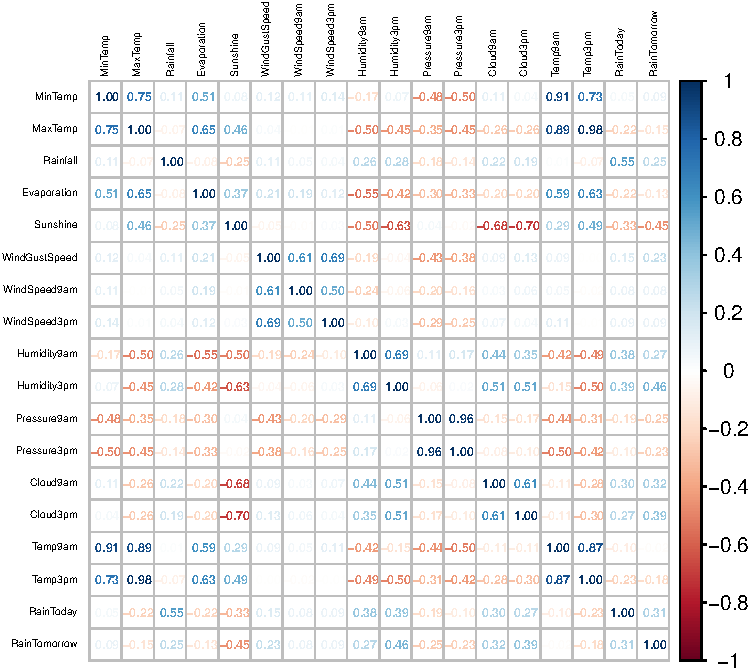
\includegraphics{Rain_Australia_files/figure-latex/correlation-1.pdf}

\hypertarget{density-plots}{%
\subsection{Density Plots}\label{density-plots}}

Based on the results of the correlation matrix, we further illustrated
the features exhibiting the highest correlation using density and bar
plots for the continuous and categorical variables, respectively against
the target variable. From these plots, we identified the following
trends: In the density plot with Sushine, we noted that the fraction of
total days having higher sunshine are associated with more 0
RainTomorrow, and lower sunshine levels with more 1 RainTomorrow;
Whereas, the Humidity3pm density plot appeared to have higher overlap
between the two classes, but still higher humidity associated with 1
RainTomorrow and vice-versa. In the density plots with the two Cloud
variables (9 am and 3 pm), we observed more oscillation across the
x-axis with higher discrepancies in the target class at the two
extremes. Finally, the representation of the RainToday binary variable
against the target variable in a bar chart expresses the strong
correlation between the classes of the two variables.We found a similar
number of samples with both RainToday and RainTomorrow equal to 0 and
vice-versa.

\begin{Shaded}
\begin{Highlighting}[]
\DocumentationTok{\#\# Find features with highest correlation with target variable (RainTomorrow)}

\NormalTok{correlations }\OtherTok{\textless{}{-}}\NormalTok{ cor\_matrix[}\StringTok{\textquotesingle{}RainTomorrow\textquotesingle{}}\NormalTok{,]}
\NormalTok{highly\_correlated\_columns }\OtherTok{\textless{}{-}}\NormalTok{ correlations[}\FunctionTok{abs}\NormalTok{(correlations) }\SpecialCharTok{\textgreater{}} \FloatTok{0.3} \SpecialCharTok{\&} 
\NormalTok{                                            correlations }\SpecialCharTok{!=} \DecValTok{1}\NormalTok{] }
\NormalTok{column\_names }\OtherTok{\textless{}{-}} \FunctionTok{names}\NormalTok{(highly\_correlated\_columns)}
\FunctionTok{print}\NormalTok{(column\_names)}
\end{Highlighting}
\end{Shaded}

\begin{verbatim}
## [1] "Sunshine"    "Humidity3pm" "Cloud9am"    "Cloud3pm"    "RainToday"
\end{verbatim}

\begin{Shaded}
\begin{Highlighting}[]
\NormalTok{rain\_subset }\OtherTok{\textless{}{-}}\NormalTok{ rain[,}\FunctionTok{c}\NormalTok{(column\_names)]}

\CommentTok{\# We are trying to visualize relationship between Target Variable, RainTomorrow }
\CommentTok{\# with the features having the highest correlation}

\CommentTok{\# Calculate the count of each feature}
\NormalTok{count\_rain\_today }\OtherTok{\textless{}{-}} \FunctionTok{sum}\NormalTok{(rain}\SpecialCharTok{$}\NormalTok{RainToday }\SpecialCharTok{==} \DecValTok{1}\NormalTok{)}
\NormalTok{count\_no\_rain\_today }\OtherTok{\textless{}{-}} \FunctionTok{sum}\NormalTok{(rain}\SpecialCharTok{$}\NormalTok{RainToday }\SpecialCharTok{==} \DecValTok{0}\NormalTok{)}
\NormalTok{count\_rain\_tomorrow }\OtherTok{\textless{}{-}} \FunctionTok{sum}\NormalTok{(rain}\SpecialCharTok{$}\NormalTok{RainTomorrow }\SpecialCharTok{==} \DecValTok{1}\NormalTok{)}
\NormalTok{count\_no\_rain\_tomorrow }\OtherTok{\textless{}{-}} \FunctionTok{sum}\NormalTok{(rain}\SpecialCharTok{$}\NormalTok{RainTomorrow }\SpecialCharTok{==} \DecValTok{0}\NormalTok{)}

\CommentTok{\# Create a data frame with the counts}
\NormalTok{count\_df }\OtherTok{\textless{}{-}} \FunctionTok{data.frame}\NormalTok{(}
  \AttributeTok{Feature =} \FunctionTok{c}\NormalTok{(}\StringTok{"RainToday"}\NormalTok{, }\StringTok{"RainTomorrow"}\NormalTok{, }\StringTok{"RainToday"}\NormalTok{,}\StringTok{"RainTomorrow"}\NormalTok{),}
  \AttributeTok{Value =} \FunctionTok{c}\NormalTok{(}\StringTok{"1"}\NormalTok{, }\StringTok{"1"}\NormalTok{, }\StringTok{"0"}\NormalTok{, }\StringTok{"0"}\NormalTok{),}
  \AttributeTok{Count =} \FunctionTok{c}\NormalTok{(count\_rain\_today, count\_rain\_tomorrow, count\_no\_rain\_today, }
\NormalTok{            count\_no\_rain\_tomorrow)}
\NormalTok{)}

\NormalTok{plot\_list }\OtherTok{\textless{}{-}} \FunctionTok{list}\NormalTok{()}

\ControlFlowTok{for}\NormalTok{ (col }\ControlFlowTok{in}\NormalTok{ column\_names) \{}
  \ControlFlowTok{if}\NormalTok{ (col }\SpecialCharTok{==} \StringTok{"RainToday"}\NormalTok{) \{}
    \CommentTok{\# Plot the barplot}
\NormalTok{    bar\_plot }\OtherTok{\textless{}{-}} \FunctionTok{ggplot}\NormalTok{(count\_df, }\FunctionTok{aes}\NormalTok{(}\AttributeTok{x =}\NormalTok{ Value, }\AttributeTok{y =}\NormalTok{ Count, }\AttributeTok{fill =}\NormalTok{ Feature)) }\SpecialCharTok{+}
    \FunctionTok{geom\_bar}\NormalTok{(}\AttributeTok{stat =} \StringTok{"identity"}\NormalTok{, }\AttributeTok{position =} \StringTok{"dodge"}\NormalTok{) }\SpecialCharTok{+}
    \FunctionTok{labs}\NormalTok{(}\AttributeTok{x =} \StringTok{"Feature"}\NormalTok{, }\AttributeTok{y =} \StringTok{"Count"}\NormalTok{, }\AttributeTok{fill =} \StringTok{""}\NormalTok{) }\SpecialCharTok{+}
    \FunctionTok{scale\_fill\_manual}\NormalTok{(}\AttributeTok{values =} \FunctionTok{c}\NormalTok{(}\StringTok{"red"}\NormalTok{, }\StringTok{"blue"}\NormalTok{), }\AttributeTok{labels =} \FunctionTok{c}\NormalTok{(}\StringTok{"RainToday"}\NormalTok{, }
                                                            \StringTok{"RainTomorrow"}\NormalTok{)) }\SpecialCharTok{+}
    \FunctionTok{theme\_minimal}\NormalTok{()}
\NormalTok{    plot\_list }\OtherTok{\textless{}{-}} \FunctionTok{append}\NormalTok{(plot\_list, }\FunctionTok{list}\NormalTok{(bar\_plot))}
\NormalTok{  \}}
  \ControlFlowTok{else}\NormalTok{ \{}
\NormalTok{    density\_plot }\OtherTok{\textless{}{-}}\NormalTok{ rain}\SpecialCharTok{\%\textgreater{}\%} \FunctionTok{ggplot}\NormalTok{(}\FunctionTok{aes}\NormalTok{(}\AttributeTok{x =}\NormalTok{ .data[[col]] , }
                                       \AttributeTok{fill =} \FunctionTok{factor}\NormalTok{(RainTomorrow))) }\SpecialCharTok{+}
    \FunctionTok{geom\_density}\NormalTok{(}\AttributeTok{alpha =} \FloatTok{0.5}\NormalTok{) }\SpecialCharTok{+}
    \FunctionTok{labs}\NormalTok{(}\AttributeTok{x =}\NormalTok{ col, }\AttributeTok{y =} \StringTok{"Density"}\NormalTok{, }\AttributeTok{fill =} \StringTok{"RainTomorrow"}\NormalTok{) }\SpecialCharTok{+}
    \FunctionTok{ggtitle}\NormalTok{(}\FunctionTok{paste}\NormalTok{(}\StringTok{"Density Plot of "}\NormalTok{, col, }\StringTok{"by Raintomorrow"}\NormalTok{)) }\SpecialCharTok{+}
    \FunctionTok{theme\_minimal}\NormalTok{() }\SpecialCharTok{+}
    \FunctionTok{theme}\NormalTok{(}\AttributeTok{plot.title =} \FunctionTok{element\_text}\NormalTok{(}\AttributeTok{hjust =} \FloatTok{0.5}\NormalTok{, }\AttributeTok{size =}\DecValTok{10}\NormalTok{))}
\NormalTok{  plot\_list }\OtherTok{\textless{}{-}} \FunctionTok{append}\NormalTok{(plot\_list, }\FunctionTok{list}\NormalTok{(density\_plot))}
\NormalTok{  \}}
  
\NormalTok{\}}

\CommentTok{\# Visualize density and bar plots}
\FunctionTok{grid.arrange}\NormalTok{(}\AttributeTok{grobs =}\NormalTok{ plot\_list, }\AttributeTok{nrow =} \DecValTok{3}\NormalTok{, }\AttributeTok{ncol =} \DecValTok{2}\NormalTok{)}
\end{Highlighting}
\end{Shaded}

\begin{flushright}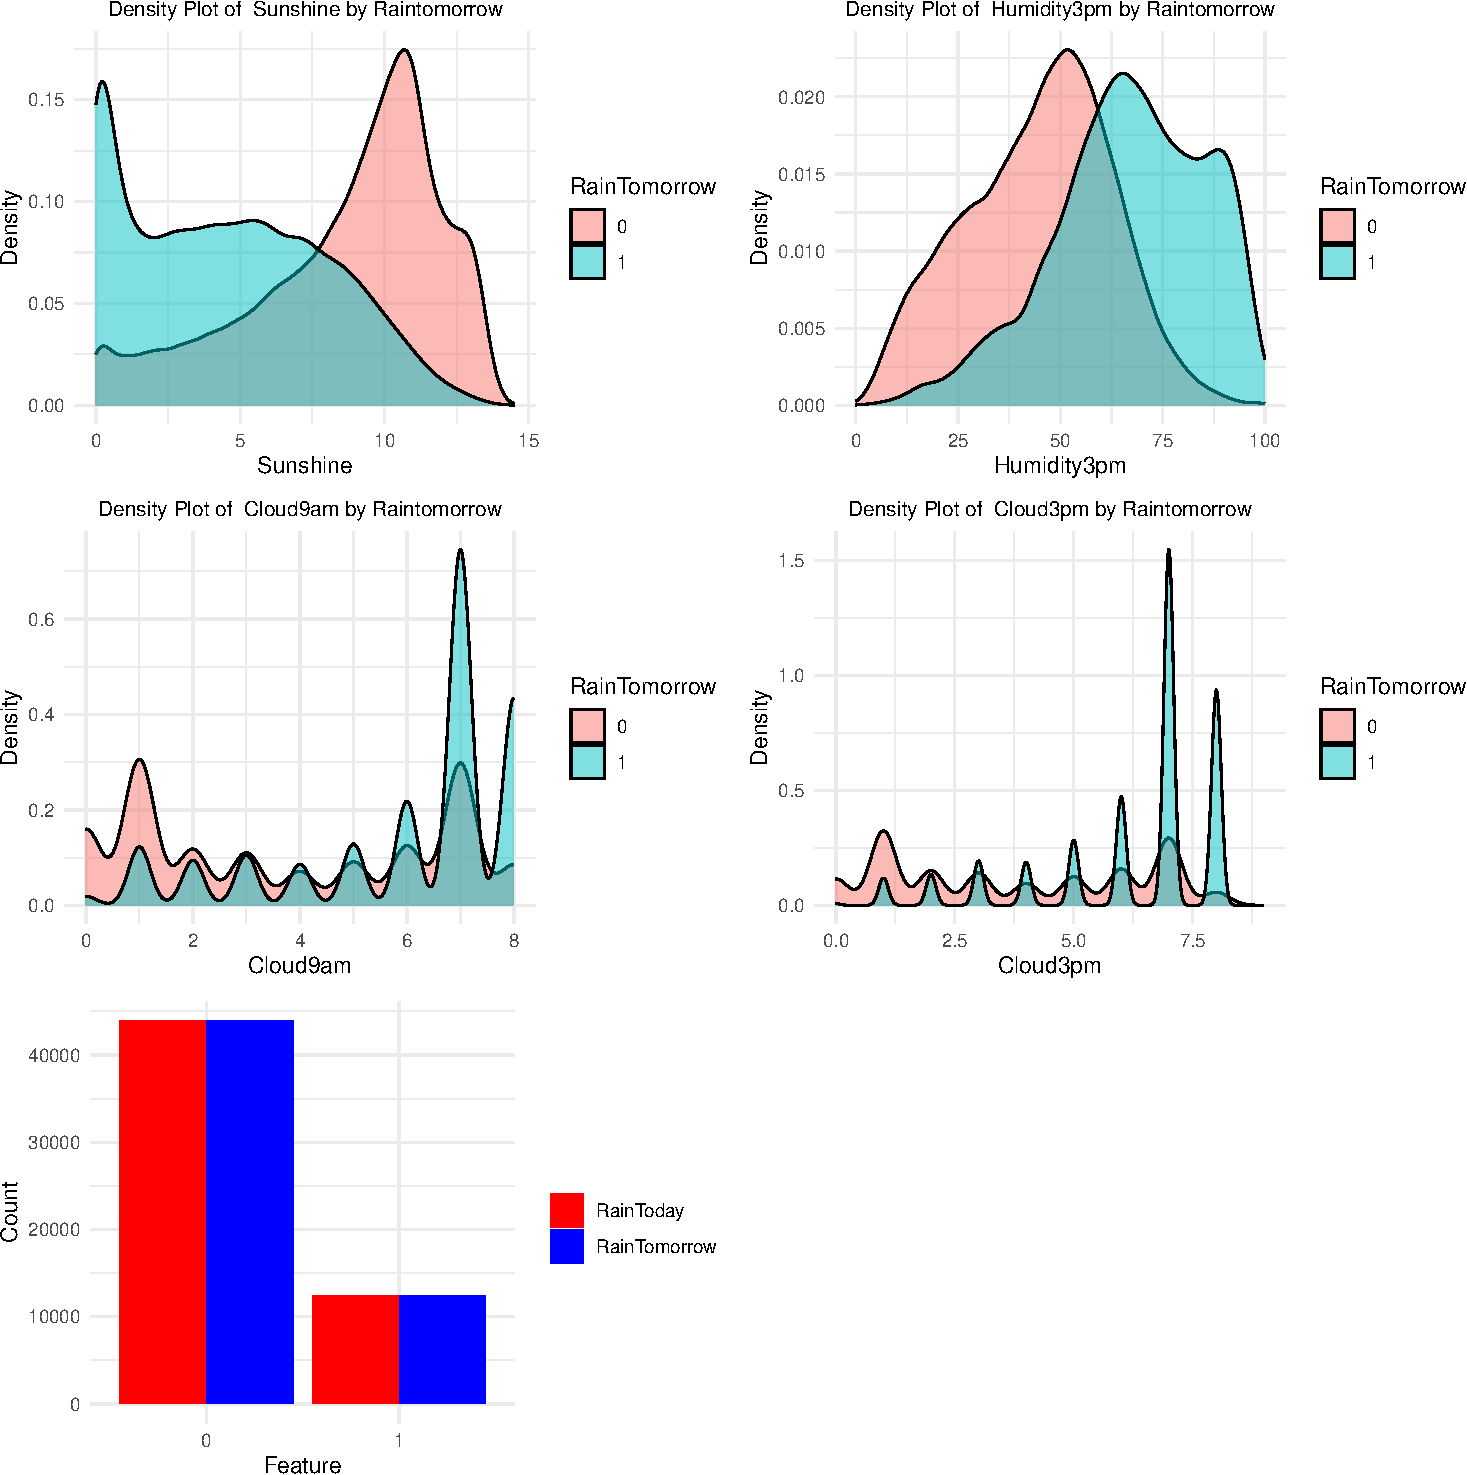
\includegraphics{Rain_Australia_files/figure-latex/density-1} \end{flushright}

\hypertarget{feature-scaling}{%
\subsection{Feature Scaling}\label{feature-scaling}}

One additional pre-processing step that is vital to statistical learning
methodologies is the application of feature scaling. Particularly when
we are creating similarity measures, i.e. Euclidean distances,
correlations, it is important to ensure your feature values fall within
a similar range. There are different feature scaling techniques to
standardize the range of feature values, but we chose min/max
normalization. The min/max scaling takes each feature value, subtracts
the minimum feature value and divides the result by the difference
between the maximum and minimum values. In our project, we applied the
min/max scaling to all the continuous variables, but kept the two binary
variables, RainToday and RainTomorrow (our target) the same.

\begin{Shaded}
\begin{Highlighting}[]
\CommentTok{\# Feature Scaling: Scale feature values using min/max scaling}
\NormalTok{min\_max\_norm }\OtherTok{\textless{}{-}} \ControlFlowTok{function}\NormalTok{(x) \{(x }\SpecialCharTok{{-}} \FunctionTok{min}\NormalTok{(x)) }\SpecialCharTok{/}\NormalTok{ (}\FunctionTok{max}\NormalTok{(x) }\SpecialCharTok{{-}} \FunctionTok{min}\NormalTok{(x))\}}

\NormalTok{rain\_n }\OtherTok{\textless{}{-}} \FunctionTok{as.data.frame}\NormalTok{(}\FunctionTok{lapply}\NormalTok{(rain[,}\DecValTok{1}\SpecialCharTok{:}\DecValTok{16}\NormalTok{], min\_max\_norm))}

\CommentTok{\#Add back in Binary Features: RainToday and target variable, RainTomorrow}
\NormalTok{rain\_n}\SpecialCharTok{$}\NormalTok{RainToday }\OtherTok{\textless{}{-}}\NormalTok{ rain}\SpecialCharTok{$}\NormalTok{RainToday}
\NormalTok{rain\_n}\SpecialCharTok{$}\NormalTok{RainTomorrow }\OtherTok{\textless{}{-}}\NormalTok{ rain}\SpecialCharTok{$}\NormalTok{RainTomorrow}
\end{Highlighting}
\end{Shaded}

\hypertarget{regression-models}{%
\section{Regression Models}\label{regression-models}}

Our primary goal for this project was to build predictive models in
order to implement a binary classification on our dataset. An intuitive
approach to achieve that is the Logistic Regression model, which is a
statistical modeling technique used to predict binary outcomes given a
set of variables. In our report, we chose to implement several versions
of this model, where we incorporated the pre-processing techniques
discussed in this report. We first started by applying a logistic
regression on the original dataset, split into a train and test sets,
with neither balancing nor feature selection. We then implemented two
other models, the first with balancing alone and the second with both
balancing and feature selection. Furthermore, to clearly see how
effective each model is, we ran predictions on the test set, plotted the
confusion matrices, and visualized different performance metrics such as
f1-score, accuracy and error. For each of these predictions, we tried
out different threshold values (0.4,0.5,0.6) for the final
classification.

\hypertarget{first-logistic-regression-model-without-balancing-or-feature-selection}{%
\subsection{First Logistic Regression Model: without balancing or
feature
selection}\label{first-logistic-regression-model-without-balancing-or-feature-selection}}

Prior to feeding our data to our model, we implemented the train/test
split which is a common machine learning technique which involves
splitting the original dataset into two subsets: the training set and
the test set. The training set is usually made up of the majority of the
dataset and is used for training, where the model learns the best
hyperparameters, without playing any part in the evaluation phase. On
the other hand, the test set is exclusively used for testing our model's
performance at predicting classes.

\begin{Shaded}
\begin{Highlighting}[]
\CommentTok{\#Train/Test Split}

\CommentTok{\#Set Seed for Reproducibility}
\FunctionTok{set.seed}\NormalTok{(}\DecValTok{123}\NormalTok{)}

\CommentTok{\# Set Training Set Size to 75\% of Total Dataset}
\NormalTok{train0 }\OtherTok{\textless{}{-}} \FunctionTok{sample}\NormalTok{(}\DecValTok{1}\SpecialCharTok{:}\FunctionTok{nrow}\NormalTok{(rain\_n), }\FunctionTok{nrow}\NormalTok{(rain\_n) }\SpecialCharTok{*} \FloatTok{0.75}\NormalTok{)}

\CommentTok{\# Calculate the test indices}
\NormalTok{test0 }\OtherTok{\textless{}{-}} \FunctionTok{setdiff}\NormalTok{(}\DecValTok{1}\SpecialCharTok{:}\FunctionTok{nrow}\NormalTok{(rain\_n), train0)}

\CommentTok{\# Split the target variable into train and test sets}
\NormalTok{rain\_n\_train0 }\OtherTok{\textless{}{-}}\NormalTok{ rain\_n[train0, ]}
\NormalTok{rain\_n\_test0 }\OtherTok{\textless{}{-}}\NormalTok{ rain\_n[test0 , ]}

\CommentTok{\# Run GLM Logistic Regression Model using Training Set}
\NormalTok{glm\_model0 }\OtherTok{\textless{}{-}} \FunctionTok{glm}\NormalTok{(}\AttributeTok{data =}\NormalTok{ rain\_n\_train0,}
\NormalTok{                  rain\_n\_train0}\SpecialCharTok{$}\NormalTok{RainTomorrow }\SpecialCharTok{\textasciitilde{}}\NormalTok{ .,}
                  \AttributeTok{family =}\NormalTok{ binomial)}

\CommentTok{\# R squared and Variance Inflation Factor (VIF)}

\CommentTok{\#R{-}squared (Coefficient of Determination): R{-}squared is a statistical metric}
\CommentTok{\#that measures the proportion of the variance in the dependent variable}
\CommentTok{\#(target variable) that can be explained by the independent variables}
\CommentTok{\#(predictor variables) in a regression model. It provides an indication of how}
\CommentTok{\#well the regression model fits the observed data.}

\CommentTok{\# VIF: is a measure used to detect multicollinearity in a regression model.}
\CommentTok{\# If the VIF value for a predictor variable is greater than 1, it indicates the}
\CommentTok{\#presence of multicollinearity, suggesting that the predictor variable is}
\CommentTok{\# highly correlated with other predictor variables in the model which makes it}
\CommentTok{\#hard to assess the individual effects of each predictor on the dependent}
\CommentTok{\#variable accurately.}


\NormalTok{model\_summary0 }\OtherTok{\textless{}{-}} \FunctionTok{summary}\NormalTok{(glm\_model0)}
\FunctionTok{summary}\NormalTok{(glm\_model0)}
\end{Highlighting}
\end{Shaded}

\begin{verbatim}
## 
## Call:
## glm(formula = rain_n_train0$RainTomorrow ~ ., family = binomial, 
##     data = rain_n_train0)
## 
## Deviance Residuals: 
##     Min       1Q   Median       3Q      Max  
## -3.0778  -0.5047  -0.2791  -0.1248   3.1273  
## 
## Coefficients:
##                Estimate Std. Error z value Pr(>|z|)    
## (Intercept)    -3.27671    0.21755 -15.062  < 2e-16 ***
## MinTemp        -1.75799    0.32913  -5.341 9.23e-08 ***
## MaxTemp         0.90140    0.60726   1.484  0.13771    
## Rainfall        2.00857    0.50309   3.992 6.54e-05 ***
## Evaporation    -0.68500    0.55112  -1.243  0.21390    
## Sunshine       -2.12269    0.10235 -20.739  < 2e-16 ***
## WindGustSpeed   7.07457    0.21145  33.458  < 2e-16 ***
## WindSpeed9am   -0.77965    0.15902  -4.903 9.44e-07 ***
## WindSpeed3pm   -2.14228    0.18900 -11.335  < 2e-16 ***
## Humidity9am     0.25419    0.18214   1.396  0.16285    
## Humidity3pm     5.62834    0.19259  29.225  < 2e-16 ***
## Pressure9am     8.41492    0.56060  15.011  < 2e-16 ***
## Pressure3pm   -12.37656    0.58288 -21.233  < 2e-16 ***
## Cloud9am       -0.10464    0.06917  -1.513  0.13036    
## Cloud3pm        0.99910    0.08537  11.703  < 2e-16 ***
## Temp9am         1.58034    0.50982   3.100  0.00194 ** 
## Temp3pm        -0.28768    0.65560  -0.439  0.66080    
## RainToday       0.47364    0.04201  11.273  < 2e-16 ***
## ---
## Signif. codes:  0 '***' 0.001 '**' 0.01 '*' 0.05 '.' 0.1 ' ' 1
## 
## (Dispersion parameter for binomial family taken to be 1)
## 
##     Null deviance: 44559  on 42314  degrees of freedom
## Residual deviance: 28080  on 42297  degrees of freedom
## AIC: 28116
## 
## Number of Fisher Scoring iterations: 6
\end{verbatim}

\begin{Shaded}
\begin{Highlighting}[]
\NormalTok{r2\_0 }\OtherTok{\textless{}{-}}
  \DecValTok{1} \SpecialCharTok{{-}}\NormalTok{ (model\_summary0}\SpecialCharTok{$}\NormalTok{deviance }\SpecialCharTok{/}\NormalTok{ model\_summary0}\SpecialCharTok{$}\NormalTok{null.deviance) }\CommentTok{\# 0.3698141}
\NormalTok{vif0 }\OtherTok{\textless{}{-}} \DecValTok{1} \SpecialCharTok{/}\NormalTok{ (}\DecValTok{1} \SpecialCharTok{{-}}\NormalTok{ r2\_0) }\CommentTok{\# 1.586833}

\CommentTok{\#Predict test using glm model}
\NormalTok{glm\_predict0 }\OtherTok{\textless{}{-}} \FunctionTok{predict}\NormalTok{(glm\_model0, rain\_n\_test0, }\AttributeTok{type =} \StringTok{"response"}\NormalTok{)}

\CommentTok{\#Convert predictions into 0,1 based on different thresholds}

\NormalTok{threshold4 }\OtherTok{\textless{}{-}} \FloatTok{0.4}
\NormalTok{threshold5 }\OtherTok{\textless{}{-}} \FloatTok{0.5}
\NormalTok{threshold6 }\OtherTok{\textless{}{-}} \FloatTok{0.6}

\NormalTok{glm\_predict\_4\_0 }\OtherTok{\textless{}{-}} \FunctionTok{ifelse}\NormalTok{(glm\_predict0 }\SpecialCharTok{\textgreater{}}\NormalTok{ threshold4, }\DecValTok{1}\NormalTok{, }\DecValTok{0}\NormalTok{)}
\NormalTok{glm\_predict\_5\_0 }\OtherTok{\textless{}{-}} \FunctionTok{ifelse}\NormalTok{(glm\_predict0 }\SpecialCharTok{\textgreater{}}\NormalTok{ threshold5, }\DecValTok{1}\NormalTok{, }\DecValTok{0}\NormalTok{)}
\NormalTok{glm\_predict\_6\_0 }\OtherTok{\textless{}{-}} \FunctionTok{ifelse}\NormalTok{(glm\_predict0 }\SpecialCharTok{\textgreater{}}\NormalTok{ threshold6, }\DecValTok{1}\NormalTok{, }\DecValTok{0}\NormalTok{)}

\CommentTok{\# Function to create a confusion matrix with F1 score, error and accuracy rate}
\CommentTok{\# A confusion matrix is a table that is often used to evaluate the performance}
\CommentTok{\# of a classification model. It provides a summary of the predicted and actual}
\CommentTok{\# values for a set of data points. The matrix allows us to assess how well the}
\CommentTok{\# model is performing in terms of correctly and incorrectly classifying the data.}
\CommentTok{\# The rows correspond to the predicted classes and the columns represent the}
\CommentTok{\# actual targets.}

\NormalTok{create\_confusion\_matrix }\OtherTok{\textless{}{-}}
  \ControlFlowTok{function}\NormalTok{(confusion\_matrix,}
\NormalTok{           threshold,}
\NormalTok{           error,}
\NormalTok{           accuracy) \{}
    \CommentTok{\# Extract the confusion matrix table}
\NormalTok{    cm\_table }\OtherTok{\textless{}{-}} \FunctionTok{as.data.frame}\NormalTok{(confusion\_matrix}\SpecialCharTok{$}\NormalTok{table)}
    
    \CommentTok{\#Extract F1 score}
\NormalTok{    f1\_score }\OtherTok{\textless{}{-}}\NormalTok{ confusion\_matrix}\SpecialCharTok{$}\NormalTok{byClass[}\StringTok{"F1"}\NormalTok{]}
    
    \CommentTok{\# Plot the confusion matrix using ggplot2}
    \FunctionTok{ggplot}\NormalTok{(}\AttributeTok{data =}\NormalTok{ cm\_table, }\FunctionTok{aes}\NormalTok{(}\AttributeTok{x =}\NormalTok{ Reference, }\AttributeTok{y =}\NormalTok{ Prediction, }\AttributeTok{fill =}\NormalTok{ Freq)) }\SpecialCharTok{+}
      \FunctionTok{geom\_tile}\NormalTok{(}\AttributeTok{color =} \StringTok{"white"}\NormalTok{) }\SpecialCharTok{+}
      \FunctionTok{geom\_text}\NormalTok{(}\FunctionTok{aes}\NormalTok{(}\AttributeTok{label =}\NormalTok{ Freq), }\AttributeTok{color =} \StringTok{"black"}\NormalTok{, }\AttributeTok{size =} \DecValTok{8}\NormalTok{) }\SpecialCharTok{+}
      \FunctionTok{scale\_fill\_gradient}\NormalTok{(}\AttributeTok{low =} \StringTok{"white"}\NormalTok{, }\AttributeTok{high =} \StringTok{"steelblue"}\NormalTok{) }\SpecialCharTok{+}
      \FunctionTok{labs}\NormalTok{(}
        \AttributeTok{title =} \FunctionTok{paste}\NormalTok{(}
          \StringTok{"Confusion Matrix for Threshold = "}\NormalTok{,}
\NormalTok{          threshold,}
          \StringTok{"with F1{-}Score:"}\NormalTok{,}
          \FunctionTok{round}\NormalTok{(f1\_score, }\DecValTok{3}\NormalTok{),}
          \StringTok{"Error:"}\NormalTok{,}
          \FunctionTok{round}\NormalTok{(error, }\DecValTok{3}\NormalTok{) ,}
          \StringTok{"Accuracy:"}\NormalTok{,}
          \FunctionTok{round}\NormalTok{(accuracy, }\DecValTok{3}\NormalTok{)}
\NormalTok{        ),}
        \AttributeTok{x =} \StringTok{"Target"}\NormalTok{,}
        \AttributeTok{y =} \StringTok{"Prediction"}
\NormalTok{      ) }\SpecialCharTok{+}
      \FunctionTok{theme\_minimal}\NormalTok{() }\SpecialCharTok{+}
      \FunctionTok{theme}\NormalTok{(}\AttributeTok{axis.text =} \FunctionTok{element\_text}\NormalTok{(}\AttributeTok{size =} \DecValTok{8}\NormalTok{),}
            \AttributeTok{plot.title =} \FunctionTok{element\_text}\NormalTok{(}\AttributeTok{size =} \DecValTok{8}\NormalTok{, }\AttributeTok{face =} \StringTok{"bold"}\NormalTok{))}
    
\NormalTok{  \}}

\CommentTok{\# Confusion matrix with threshold = 0.4}
\NormalTok{error4\_0 }\OtherTok{\textless{}{-}} \FunctionTok{mean}\NormalTok{(glm\_predict\_4\_0 }\SpecialCharTok{!=}\NormalTok{ rain\_n\_test0}\SpecialCharTok{$}\NormalTok{RainTomorrow)}
\NormalTok{accuracy4\_0 }\OtherTok{\textless{}{-}} \FunctionTok{mean}\NormalTok{(glm\_predict\_4\_0 }\SpecialCharTok{==}\NormalTok{ rain\_n\_test0}\SpecialCharTok{$}\NormalTok{RainTomorrow)}
\NormalTok{cm4\_0 }\OtherTok{\textless{}{-}}
  \FunctionTok{confusionMatrix}\NormalTok{(}
    \AttributeTok{data =} \FunctionTok{factor}\NormalTok{(glm\_predict\_4\_0),}
    \AttributeTok{reference =} \FunctionTok{factor}\NormalTok{(rain\_n\_test0}\SpecialCharTok{$}\NormalTok{RainTomorrow),}
    \AttributeTok{mode =} \StringTok{\textquotesingle{}everything\textquotesingle{}}
\NormalTok{  )}

\CommentTok{\# Confusion matrix with threshold = 0.5}
\NormalTok{error5\_0 }\OtherTok{\textless{}{-}} \FunctionTok{mean}\NormalTok{(glm\_predict\_5\_0 }\SpecialCharTok{!=}\NormalTok{ rain\_n\_test0}\SpecialCharTok{$}\NormalTok{RainTomorrow)}
\NormalTok{accuracy5\_0 }\OtherTok{\textless{}{-}} \FunctionTok{mean}\NormalTok{(glm\_predict\_5\_0 }\SpecialCharTok{==}\NormalTok{ rain\_n\_test0}\SpecialCharTok{$}\NormalTok{RainTomorrow)}
\NormalTok{cm5\_0 }\OtherTok{\textless{}{-}}
  \FunctionTok{confusionMatrix}\NormalTok{(}
    \AttributeTok{data =} \FunctionTok{factor}\NormalTok{(glm\_predict\_5\_0),}
    \AttributeTok{reference =} \FunctionTok{factor}\NormalTok{(rain\_n\_test0}\SpecialCharTok{$}\NormalTok{RainTomorrow),}
    \AttributeTok{mode =} \StringTok{\textquotesingle{}everything\textquotesingle{}}
\NormalTok{  )}

\CommentTok{\# Confusion matrix with threshold = 0.6}
\NormalTok{error6\_0 }\OtherTok{\textless{}{-}} \FunctionTok{mean}\NormalTok{(glm\_predict\_6\_0 }\SpecialCharTok{!=}\NormalTok{ rain\_n\_test0}\SpecialCharTok{$}\NormalTok{RainTomorrow)}
\NormalTok{accuracy6\_0 }\OtherTok{\textless{}{-}} \FunctionTok{mean}\NormalTok{(glm\_predict\_6\_0 }\SpecialCharTok{==}\NormalTok{ rain\_n\_test0}\SpecialCharTok{$}\NormalTok{RainTomorrow)}
\NormalTok{cm6\_0 }\OtherTok{\textless{}{-}}
  \FunctionTok{confusionMatrix}\NormalTok{(}
    \AttributeTok{data =} \FunctionTok{factor}\NormalTok{(glm\_predict\_6\_0),}
    \AttributeTok{reference =} \FunctionTok{factor}\NormalTok{(rain\_n\_test0}\SpecialCharTok{$}\NormalTok{RainTomorrow),}
    \AttributeTok{mode =} \StringTok{\textquotesingle{}everything\textquotesingle{}}
\NormalTok{  )}

\NormalTok{a0 }\OtherTok{\textless{}{-}} \FunctionTok{create\_confusion\_matrix}\NormalTok{(cm4\_0, }\FloatTok{0.4}\NormalTok{, error4\_0, accuracy4\_0)}
\NormalTok{b0 }\OtherTok{\textless{}{-}} \FunctionTok{create\_confusion\_matrix}\NormalTok{(cm5\_0, }\FloatTok{0.5}\NormalTok{, error5\_0, accuracy5\_0)}
\NormalTok{c0 }\OtherTok{\textless{}{-}} \FunctionTok{create\_confusion\_matrix}\NormalTok{(cm6\_0, }\FloatTok{0.6}\NormalTok{, error6\_0, accuracy6\_0)}

\CommentTok{\# Threshold of 0.05 is the best among thresholds in terms of accuracy,}
\CommentTok{\#sensitivity, and specificity}
\NormalTok{cm\_all0 }\OtherTok{=} \FunctionTok{list}\NormalTok{(a0, b0, c0)}
\NormalTok{plot\_width }\OtherTok{\textless{}{-}} \FunctionTok{c}\NormalTok{(}\DecValTok{4}\NormalTok{, }\DecValTok{4}\NormalTok{, }\DecValTok{4}\NormalTok{)}
\FunctionTok{grid.arrange}\NormalTok{(}\AttributeTok{grobs =}\NormalTok{ cm\_all0,}
             \AttributeTok{nrow =} \DecValTok{3}\NormalTok{,}
             \AttributeTok{width =}\NormalTok{ plot\_width)}
\end{Highlighting}
\end{Shaded}

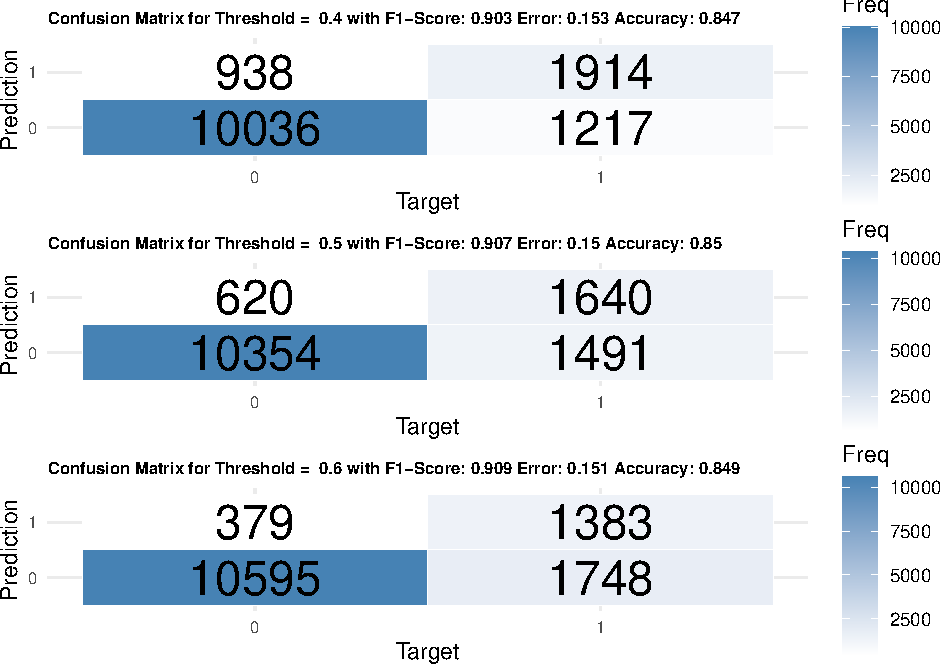
\includegraphics{Rain_Australia_files/figure-latex/log. regression w/o balancing or feature selection-1.pdf}

\hypertarget{logistic-regression-with-balancing}{%
\subsection{Logistic Regression with
Balancing}\label{logistic-regression-with-balancing}}

In addition to feature scaling, balancing our data is another technique
used to prepare data before applying predictive modeling. Balancing
reduces the effect of the dominating class which results in high bias
and unreliable predictions. In order to balance data, there are several
under-sampling and over-sampling methods that can be used depending on
the characteristics of the dataset. As we will observe in the code
below, our original data isn't balanced, in which 0 is the majority
class with over 40,000 and 1 has only about 12,000 samples. To account
for this imbalance, we performed a method of under-sampling, whereby we
reduced the number of samples in the majority class (0) to the same
number of samples of the minority class (1). This methodology may reduce
the pool of data we have available, but it removes the bias in our model
predictions toward one dominating class. We opted against using
over-sampling as that might add unwanted noise to our data which might
also lead to unreliable results.

\begin{Shaded}
\begin{Highlighting}[]
\CommentTok{\# Check distribution of RainTomorrow values to see how balanced the data is}
\CommentTok{\# 0: 43993; 1: 12427}
\FunctionTok{table}\NormalTok{(rain}\SpecialCharTok{$}\NormalTok{RainTomorrow)}
\end{Highlighting}
\end{Shaded}

\begin{verbatim}
## 
##     0     1 
## 43993 12427
\end{verbatim}

\begin{Shaded}
\begin{Highlighting}[]
\CommentTok{\#Downsamples majority class(0)}
\CommentTok{\#Added yname to specify the target variable in downSample function, ow it }
\CommentTok{\#assumes first col is target}
\NormalTok{rain\_balanced }\OtherTok{\textless{}{-}}
  \FunctionTok{downSample}\NormalTok{(}\AttributeTok{x =}\NormalTok{ rain\_n[,}\SpecialCharTok{{-}}\FunctionTok{which}\NormalTok{(}\FunctionTok{names}\NormalTok{(rain\_n) }\SpecialCharTok{==} \StringTok{"RainTomorrow"}\NormalTok{)],}
             \AttributeTok{y =} \FunctionTok{factor}\NormalTok{(rain\_n}\SpecialCharTok{$}\NormalTok{RainTomorrow),}
             \AttributeTok{yname =} \StringTok{"RainTomorrow"}\NormalTok{)}
\FunctionTok{table}\NormalTok{(rain\_balanced}\SpecialCharTok{$}\NormalTok{RainTomorrow)}
\end{Highlighting}
\end{Shaded}

\begin{verbatim}
## 
##     0     1 
## 12427 12427
\end{verbatim}

\begin{Shaded}
\begin{Highlighting}[]
\FunctionTok{head}\NormalTok{(rain\_balanced)}
\end{Highlighting}
\end{Shaded}

\begin{verbatim}
##     MinTemp   MaxTemp    Rainfall Evaporation  Sunshine WindGustSpeed
## 1 0.6692913 0.4409091 0.007759457  0.06896552 0.1172414     0.2608696
## 2 0.8661417 0.6772727 0.000000000  0.08374384 0.7034483     0.2260870
## 3 0.4094488 0.5204545 0.000000000  0.06403941 0.5931034     0.2434783
## 4 0.7086614 0.6750000 0.000000000  0.09852217 0.6275862     0.3565217
## 5 0.5301837 0.6795455 0.000000000  0.11822660 0.6275862     0.2782609
## 6 0.6141732 0.4886364 0.000000000  0.08128079 0.7103448     0.2782609
##   WindSpeed9am WindSpeed3pm Humidity9am Humidity3pm Pressure9am Pressure3pm
## 1    0.2307692    0.2432432        0.64        0.71   0.6494157   0.6521036
## 2    0.2000000    0.3513514        0.72        0.59   0.5358932   0.5129450
## 3    0.1076923    0.2702703        0.72        0.45   0.6961603   0.6618123
## 4    0.3076923    0.2297297        0.60        0.45   0.4741235   0.4854369
## 5    0.1076923    0.1486486        0.32        0.18   0.5225376   0.5339806
## 6    0.2615385    0.2297297        0.76        0.45   0.5409015   0.5679612
##   Cloud9am  Cloud3pm   Temp9am   Temp3pm RainToday RainTomorrow
## 1    0.875 0.7777778 0.5810474 0.4363208         1            0
## 2    0.250 0.2222222 0.7605985 0.6816038         0            0
## 3    0.625 0.3333333 0.4738155 0.5188679         0            0
## 4    0.625 0.6666667 0.6832918 0.6698113         0            0
## 5    0.750 0.5555556 0.5960100 0.6297170         0            0
## 6    1.000 0.1111111 0.4588529 0.4740566         0            0
\end{verbatim}

\begin{Shaded}
\begin{Highlighting}[]
\CommentTok{\#Check if there are any NAs}
\FunctionTok{sum}\NormalTok{(}\FunctionTok{is.na}\NormalTok{(rain\_balanced}\SpecialCharTok{$}\NormalTok{RainTomorrow))}
\end{Highlighting}
\end{Shaded}

\begin{verbatim}
## [1] 0
\end{verbatim}

\begin{Shaded}
\begin{Highlighting}[]
\CommentTok{\#Test/Train Split}
\FunctionTok{set.seed}\NormalTok{(}\DecValTok{123}\NormalTok{)}

\NormalTok{train\_balanced }\OtherTok{\textless{}{-}}
  \FunctionTok{sample}\NormalTok{(}\DecValTok{1}\SpecialCharTok{:}\FunctionTok{nrow}\NormalTok{(rain\_balanced), }\FunctionTok{nrow}\NormalTok{(rain\_balanced) }\SpecialCharTok{*} \FloatTok{0.75}\NormalTok{)}

\CommentTok{\# Calculate the test indices}
\NormalTok{test\_balanced }\OtherTok{\textless{}{-}} \FunctionTok{setdiff}\NormalTok{(}\DecValTok{1}\SpecialCharTok{:}\FunctionTok{nrow}\NormalTok{(rain\_balanced), train\_balanced)}

\CommentTok{\# Split the target variable into train and test sets}
\NormalTok{rain\_balanced\_train }\OtherTok{\textless{}{-}}\NormalTok{ rain\_balanced[train\_balanced, ]}
\NormalTok{rain\_balanced\_test }\OtherTok{\textless{}{-}}\NormalTok{ rain\_balanced[test\_balanced , ]}
\NormalTok{glm\_model\_balanced }\OtherTok{\textless{}{-}} \FunctionTok{glm}\NormalTok{(}\AttributeTok{data =}\NormalTok{ rain\_balanced\_train,}
\NormalTok{                          rain\_balanced\_train}\SpecialCharTok{$}\NormalTok{RainTomorrow }\SpecialCharTok{\textasciitilde{}}\NormalTok{ .,}
                          \AttributeTok{family =}\NormalTok{ binomial)}

\NormalTok{model\_summary\_balanced }\OtherTok{\textless{}{-}} \FunctionTok{summary}\NormalTok{(glm\_model\_balanced)}
\FunctionTok{summary}\NormalTok{(glm\_model\_balanced)}
\end{Highlighting}
\end{Shaded}

\begin{verbatim}
## 
## Call:
## glm(formula = rain_balanced_train$RainTomorrow ~ ., family = binomial, 
##     data = rain_balanced_train)
## 
## Deviance Residuals: 
##     Min       1Q   Median       3Q      Max  
## -3.5064  -0.6447   0.0516   0.6418   2.8163  
## 
## Coefficients:
##                Estimate Std. Error z value Pr(>|z|)    
## (Intercept)    -1.78587    0.28387  -6.291 3.15e-10 ***
## MinTemp        -1.45819    0.41703  -3.497 0.000471 ***
## MaxTemp         1.04710    0.84911   1.233 0.217513    
## Rainfall        1.47028    0.77973   1.886 0.059346 .  
## Evaporation    -1.42725    0.70721  -2.018 0.043577 *  
## Sunshine       -2.57528    0.13469 -19.119  < 2e-16 ***
## WindGustSpeed   6.91036    0.29248  23.627  < 2e-16 ***
## WindSpeed9am   -0.64221    0.21128  -3.040 0.002369 ** 
## WindSpeed3pm   -1.72241    0.25163  -6.845 7.65e-12 ***
## Humidity9am     0.19478    0.23371   0.833 0.404623    
## Humidity3pm     5.68413    0.25584  22.217  < 2e-16 ***
## Pressure9am     8.31613    0.75726  10.982  < 2e-16 ***
## Pressure3pm   -12.46658    0.79195 -15.742  < 2e-16 ***
## Cloud9am       -0.27995    0.08624  -3.246 0.001169 ** 
## Cloud3pm        1.07058    0.10368  10.325  < 2e-16 ***
## Temp9am         0.49761    0.65435   0.760 0.446979    
## Temp3pm         0.73571    0.89965   0.818 0.413484    
## RainToday       0.46663    0.05825   8.011 1.14e-15 ***
## ---
## Signif. codes:  0 '***' 0.001 '**' 0.01 '*' 0.05 '.' 0.1 ' ' 1
## 
## (Dispersion parameter for binomial family taken to be 1)
## 
##     Null deviance: 25840  on 18639  degrees of freedom
## Residual deviance: 15893  on 18622  degrees of freedom
## AIC: 15929
## 
## Number of Fisher Scoring iterations: 5
\end{verbatim}

\begin{Shaded}
\begin{Highlighting}[]
\NormalTok{r2\_balanced }\OtherTok{\textless{}{-}}
  \DecValTok{1} \SpecialCharTok{{-}}\NormalTok{ (model\_summary\_balanced}\SpecialCharTok{$}\NormalTok{deviance }\SpecialCharTok{/}\NormalTok{ model\_summary\_balanced}\SpecialCharTok{$}\NormalTok{null.deviance) }
\CommentTok{\# 0.3849359}
\NormalTok{vif\_balanced }\OtherTok{\textless{}{-}} \DecValTok{1} \SpecialCharTok{/}\NormalTok{ (}\DecValTok{1} \SpecialCharTok{{-}}\NormalTok{ r2\_balanced) }\CommentTok{\# 1.625847}

\CommentTok{\#Predict test with model}
\NormalTok{glm\_predict\_balanced }\OtherTok{\textless{}{-}}
  \FunctionTok{predict}\NormalTok{(glm\_model\_balanced, rain\_balanced\_test, }\AttributeTok{type =} \StringTok{"response"}\NormalTok{)}

\CommentTok{\#Convert predictions into 0,1 based on different thresholds}

\NormalTok{glm\_predict\_4\_balanced }\OtherTok{\textless{}{-}}
  \FunctionTok{ifelse}\NormalTok{(glm\_predict\_balanced }\SpecialCharTok{\textgreater{}}\NormalTok{ threshold4, }\DecValTok{1}\NormalTok{, }\DecValTok{0}\NormalTok{)}
\NormalTok{glm\_predict\_5\_balanced }\OtherTok{\textless{}{-}}
  \FunctionTok{ifelse}\NormalTok{(glm\_predict\_balanced }\SpecialCharTok{\textgreater{}}\NormalTok{ threshold5, }\DecValTok{1}\NormalTok{, }\DecValTok{0}\NormalTok{)}
\NormalTok{glm\_predict\_6\_balanced }\OtherTok{\textless{}{-}}
  \FunctionTok{ifelse}\NormalTok{(glm\_predict\_balanced }\SpecialCharTok{\textgreater{}}\NormalTok{ threshold6, }\DecValTok{1}\NormalTok{, }\DecValTok{0}\NormalTok{)}

\CommentTok{\# Confusion matrix with threshold = 0.4}
\FunctionTok{table}\NormalTok{(rain\_balanced\_test}\SpecialCharTok{$}\NormalTok{RainTomorrow, glm\_predict\_4\_balanced)}
\end{Highlighting}
\end{Shaded}

\begin{verbatim}
##    glm_predict_4_balanced
##        0    1
##   0 2335  798
##   1  446 2635
\end{verbatim}

\begin{Shaded}
\begin{Highlighting}[]
\NormalTok{error4\_balanced }\OtherTok{\textless{}{-}}
  \FunctionTok{mean}\NormalTok{(glm\_predict\_4\_balanced }\SpecialCharTok{!=}\NormalTok{ rain\_balanced\_test}\SpecialCharTok{$}\NormalTok{RainTomorrow)}
\NormalTok{accuracy4\_balanced }\OtherTok{\textless{}{-}}
  \FunctionTok{mean}\NormalTok{(glm\_predict\_4\_balanced }\SpecialCharTok{==}\NormalTok{ rain\_balanced\_test}\SpecialCharTok{$}\NormalTok{RainTomorrow)}
\NormalTok{cm4\_balanced }\OtherTok{\textless{}{-}}
  \FunctionTok{confusionMatrix}\NormalTok{(}
    \AttributeTok{data =} \FunctionTok{factor}\NormalTok{(glm\_predict\_4\_balanced),}
    \AttributeTok{reference =} \FunctionTok{factor}\NormalTok{(rain\_balanced\_test}\SpecialCharTok{$}\NormalTok{RainTomorrow),}
    \AttributeTok{mode =} \StringTok{\textquotesingle{}everything\textquotesingle{}}
\NormalTok{  )}

\CommentTok{\# Confusion matrix with threshold = 0.5}
\FunctionTok{table}\NormalTok{(rain\_balanced\_test}\SpecialCharTok{$}\NormalTok{RainTomorrow, glm\_predict\_5\_balanced)}
\end{Highlighting}
\end{Shaded}

\begin{verbatim}
##    glm_predict_5_balanced
##        0    1
##   0 2528  605
##   1  649 2432
\end{verbatim}

\begin{Shaded}
\begin{Highlighting}[]
\NormalTok{error5\_balanced }\OtherTok{\textless{}{-}}
  \FunctionTok{mean}\NormalTok{(glm\_predict\_5\_balanced }\SpecialCharTok{!=}\NormalTok{ rain\_balanced\_test}\SpecialCharTok{$}\NormalTok{RainTomorrow)}
\NormalTok{accuracy5\_balanced }\OtherTok{\textless{}{-}}
  \FunctionTok{mean}\NormalTok{(glm\_predict\_5\_balanced }\SpecialCharTok{==}\NormalTok{ rain\_balanced\_test}\SpecialCharTok{$}\NormalTok{RainTomorrow)}
\NormalTok{cm5\_balanced }\OtherTok{\textless{}{-}}
  \FunctionTok{confusionMatrix}\NormalTok{(}
    \AttributeTok{data =} \FunctionTok{factor}\NormalTok{(glm\_predict\_5\_balanced),}
    \AttributeTok{reference =} \FunctionTok{factor}\NormalTok{(rain\_balanced\_test}\SpecialCharTok{$}\NormalTok{RainTomorrow),}
    \AttributeTok{mode =} \StringTok{\textquotesingle{}everything\textquotesingle{}}
\NormalTok{  )}

\CommentTok{\# Confusion matrix with threshold = 0.6}
\FunctionTok{table}\NormalTok{(rain\_balanced\_test}\SpecialCharTok{$}\NormalTok{RainTomorrow, glm\_predict\_6\_balanced)}
\end{Highlighting}
\end{Shaded}

\begin{verbatim}
##    glm_predict_6_balanced
##        0    1
##   0 2694  439
##   1  895 2186
\end{verbatim}

\begin{Shaded}
\begin{Highlighting}[]
\NormalTok{error6\_balanced }\OtherTok{\textless{}{-}}
  \FunctionTok{mean}\NormalTok{(glm\_predict\_6\_balanced }\SpecialCharTok{!=}\NormalTok{ rain\_balanced\_test}\SpecialCharTok{$}\NormalTok{RainTomorrow)}
\NormalTok{accuracy6\_balanced }\OtherTok{\textless{}{-}}
  \FunctionTok{mean}\NormalTok{(glm\_predict\_6\_balanced }\SpecialCharTok{==}\NormalTok{ rain\_balanced\_test}\SpecialCharTok{$}\NormalTok{RainTomorrow)}
\NormalTok{cm6\_balanced }\OtherTok{\textless{}{-}}
  \FunctionTok{confusionMatrix}\NormalTok{(}
    \AttributeTok{data =} \FunctionTok{factor}\NormalTok{(glm\_predict\_6\_balanced),}
    \AttributeTok{reference =} \FunctionTok{factor}\NormalTok{(rain\_balanced\_test}\SpecialCharTok{$}\NormalTok{RainTomorrow),}
    \AttributeTok{mode =} \StringTok{\textquotesingle{}everything\textquotesingle{}}
\NormalTok{  )}

\NormalTok{a\_balanced }\OtherTok{\textless{}{-}}
  \FunctionTok{create\_confusion\_matrix}\NormalTok{(cm4\_balanced, }\FloatTok{0.4}\NormalTok{, error4\_balanced, accuracy4\_balanced)}
\NormalTok{b\_balanced }\OtherTok{\textless{}{-}}
  \FunctionTok{create\_confusion\_matrix}\NormalTok{(cm5\_balanced, }\FloatTok{0.5}\NormalTok{, error5\_balanced, accuracy5\_balanced)}
\NormalTok{c\_balanced }\OtherTok{\textless{}{-}}
  \FunctionTok{create\_confusion\_matrix}\NormalTok{(cm6\_balanced, }\FloatTok{0.6}\NormalTok{, error6\_balanced, accuracy6\_balanced)}

\CommentTok{\# Threshold of 0.5 is the best among thresholds in terms of accuracy, }
\CommentTok{\#sensitivity, and specificity}
\NormalTok{cm\_all\_balanced }\OtherTok{=} \FunctionTok{list}\NormalTok{(a\_balanced, b\_balanced, c\_balanced)}
\NormalTok{plot\_width }\OtherTok{\textless{}{-}} \FunctionTok{c}\NormalTok{(}\DecValTok{4}\NormalTok{, }\DecValTok{4}\NormalTok{, }\DecValTok{4}\NormalTok{)}
\FunctionTok{grid.arrange}\NormalTok{(}\AttributeTok{grobs =}\NormalTok{ cm\_all\_balanced,}
             \AttributeTok{nrow =} \DecValTok{3}\NormalTok{,}
             \AttributeTok{width =}\NormalTok{ plot\_width)}
\end{Highlighting}
\end{Shaded}

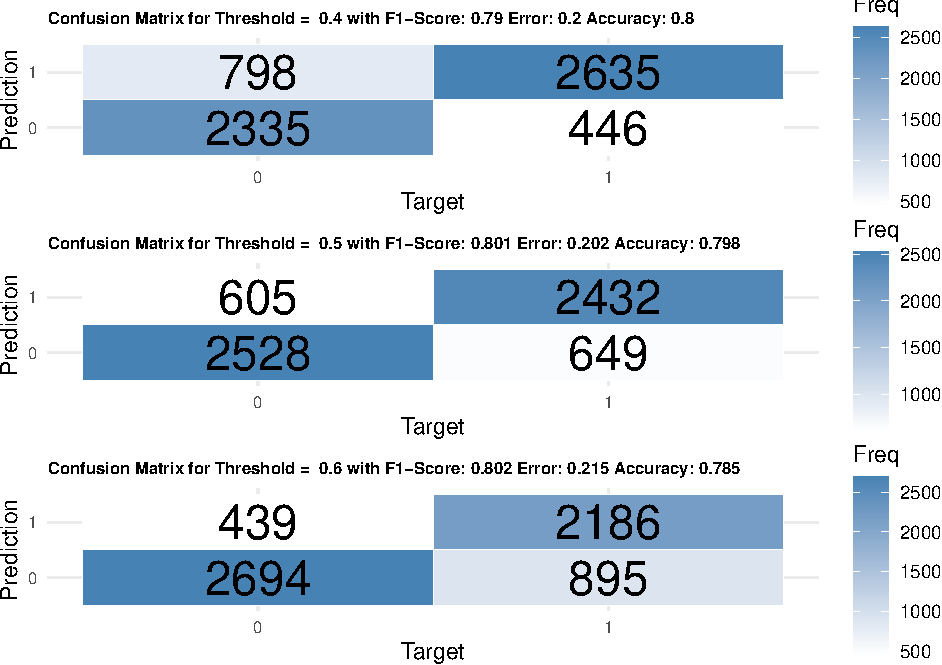
\includegraphics{Rain_Australia_files/figure-latex/log. regression pre feature selection-1.pdf}

\hypertarget{logistic-regression-with-feature-selection}{%
\subsection{Logistic Regression with Feature
Selection}\label{logistic-regression-with-feature-selection}}

Feature selection is another key step in predictive model definition.
The selection method involves evaluating all the features provided in
the original dataset and selecting the most relevant features that best
describe and predict our data. By identifying a smaller subset of
important features, we are ensuring that the model doesn't overfit on
the training data and is able to generalize on new data. Several
techniques can be implemented to apply feature selection. Forward and
backward selection iterate through all the features to determine each
feature's effect on the overall model by cumulatively adding features
from an empty set or removing features one at a time from the full set,
respectively. Moreover, the two methods can be integrated to obtain a
more exhaustive feature selection. Within the configuration of forward
and backward selection using Akaike Information Criterion (AIC) or
Bayesian Information Criterion (BIC), you can select the degree of
penalization for the amount of features through the choice of k. The
penalty term increases proportionally with the number of parameters set
by k, which ensures that the complexity of the model is taken into
account and to avoid overfitting. We chose to configure backward
selection using BIC, which incorporates a log term and penalizes complex
models more than AIC.

\hypertarget{feature-selection-backward-selection-using-bic}{%
\subsubsection{Feature Selection (Backward Selection using
BIC)}\label{feature-selection-backward-selection-using-bic}}

\begin{Shaded}
\begin{Highlighting}[]
\CommentTok{\# Perform logistic regression with backward stepwise selection}
\NormalTok{logit\_model }\OtherTok{\textless{}{-}}
  \FunctionTok{glm}\NormalTok{(rain\_balanced}\SpecialCharTok{$}\NormalTok{RainTomorrow }\SpecialCharTok{\textasciitilde{}}\NormalTok{ .,}
      \AttributeTok{data =}\NormalTok{ rain\_balanced,}
      \AttributeTok{family =}\NormalTok{ binomial)}

\CommentTok{\# Perform forward stepwise selection using BIC with log(n)}
\NormalTok{logit\_model }\OtherTok{\textless{}{-}}
  \FunctionTok{stepAIC}\NormalTok{(}
\NormalTok{    logit\_model,}
    \AttributeTok{direction =} \StringTok{"backward"}\NormalTok{,}
    \AttributeTok{k =} \FunctionTok{log}\NormalTok{(}\FunctionTok{nrow}\NormalTok{(rain\_balanced)),}
    \AttributeTok{trace =} \ConstantTok{FALSE}
\NormalTok{  )}

\CommentTok{\# Print the summary of the logistic regression model}
\FunctionTok{summary}\NormalTok{(logit\_model)}
\end{Highlighting}
\end{Shaded}

\begin{verbatim}
## 
## Call:
## glm(formula = rain_balanced$RainTomorrow ~ MinTemp + MaxTemp + 
##     Rainfall + Sunshine + WindGustSpeed + WindSpeed9am + WindSpeed3pm + 
##     Humidity3pm + Pressure9am + Pressure3pm + Cloud9am + Cloud3pm + 
##     RainToday, family = binomial, data = rain_balanced)
## 
## Deviance Residuals: 
##     Min       1Q   Median       3Q      Max  
## -3.5377  -0.6440  -0.0412   0.6411   2.8180  
## 
## Coefficients:
##                Estimate Std. Error z value Pr(>|z|)    
## (Intercept)    -1.63412    0.22495  -7.264 3.74e-13 ***
## MinTemp        -1.01052    0.24797  -4.075 4.60e-05 ***
## MaxTemp         1.39711    0.30809   4.535 5.77e-06 ***
## Rainfall        2.29815    0.69305   3.316 0.000913 ***
## Sunshine       -2.36985    0.11567 -20.488  < 2e-16 ***
## WindGustSpeed   7.04107    0.24971  28.197  < 2e-16 ***
## WindSpeed9am   -0.81429    0.17622  -4.621 3.82e-06 ***
## WindSpeed3pm   -1.98642    0.21483  -9.246  < 2e-16 ***
## Humidity3pm     5.76180    0.15339  37.562  < 2e-16 ***
## Pressure9am     8.78896    0.61661  14.254  < 2e-16 ***
## Pressure3pm   -13.07527    0.64902 -20.146  < 2e-16 ***
## Cloud9am       -0.25366    0.07282  -3.483 0.000495 ***
## Cloud3pm        1.11010    0.08919  12.447  < 2e-16 ***
## RainToday       0.47366    0.04919   9.629  < 2e-16 ***
## ---
## Signif. codes:  0 '***' 0.001 '**' 0.01 '*' 0.05 '.' 0.1 ' ' 1
## 
## (Dispersion parameter for binomial family taken to be 1)
## 
##     Null deviance: 34455  on 24853  degrees of freedom
## Residual deviance: 21168  on 24840  degrees of freedom
## AIC: 21196
## 
## Number of Fisher Scoring iterations: 5
\end{verbatim}

\begin{Shaded}
\begin{Highlighting}[]
\CommentTok{\# Subset the dataframe with the chosen features based on stepwise selection}
\NormalTok{rain\_subset }\OtherTok{\textless{}{-}}
\NormalTok{  rain\_balanced[, }\FunctionTok{c}\NormalTok{(}
    \StringTok{"MinTemp"}\NormalTok{,}
    \StringTok{"Sunshine"}\NormalTok{,}
    \StringTok{"WindGustSpeed"}\NormalTok{,}
    \StringTok{"WindSpeed9am"}\NormalTok{,}
    \StringTok{"WindSpeed3pm"}\NormalTok{,}
    \StringTok{"Humidity3pm"}\NormalTok{,}
    \StringTok{"Pressure9am"}\NormalTok{,}
    \StringTok{"Pressure3pm"}\NormalTok{,}
    \StringTok{"Cloud9am"}\NormalTok{,}
    \StringTok{"Cloud3pm"}\NormalTok{,}
    \StringTok{"Temp3pm"}\NormalTok{,}
    \StringTok{"RainToday"}\NormalTok{,}
    \StringTok{"RainTomorrow"}
\NormalTok{  )]}
\end{Highlighting}
\end{Shaded}

\hypertarget{feature-selection-results-and-traintest-split}{%
\subsubsection{Feature Selection Results and Train/Test
Split}\label{feature-selection-results-and-traintest-split}}

In the summary of the feature selection model, we noticed that all the
features chosen had a very significant p-value (***: p close to 0).
Therefore, we decided to move forward with all the selected features we
received from backward stepwise selection in subsequent areas of the
project.

\begin{Shaded}
\begin{Highlighting}[]
\FunctionTok{set.seed}\NormalTok{(}\DecValTok{123}\NormalTok{)}

\NormalTok{train }\OtherTok{\textless{}{-}} \FunctionTok{sample}\NormalTok{(}\DecValTok{1}\SpecialCharTok{:}\FunctionTok{nrow}\NormalTok{(rain\_subset), }\FunctionTok{nrow}\NormalTok{(rain\_subset) }\SpecialCharTok{*} \FloatTok{0.75}\NormalTok{)}

\CommentTok{\# Calculate the test indices}
\NormalTok{test }\OtherTok{\textless{}{-}} \FunctionTok{setdiff}\NormalTok{(}\DecValTok{1}\SpecialCharTok{:}\FunctionTok{nrow}\NormalTok{(rain\_subset), train)}

\CommentTok{\# Split the target variable into train and test sets}
\NormalTok{rain\_subset\_train }\OtherTok{\textless{}{-}}\NormalTok{ rain\_subset[train,]}
\NormalTok{rain\_subset\_test }\OtherTok{\textless{}{-}}\NormalTok{ rain\_subset[test,]}
\end{Highlighting}
\end{Shaded}

\hypertarget{logistic-regression-using-selected-model}{%
\subsubsection{Logistic Regression using Selected
Model}\label{logistic-regression-using-selected-model}}

\begin{Shaded}
\begin{Highlighting}[]
\CommentTok{\# Model Definition}
\NormalTok{glm\_model }\OtherTok{\textless{}{-}} \FunctionTok{glm}\NormalTok{(}\AttributeTok{data =}\NormalTok{ rain\_subset\_train, }
\NormalTok{        rain\_subset\_train}\SpecialCharTok{$}\NormalTok{RainTomorrow }\SpecialCharTok{\textasciitilde{}}\NormalTok{ ., }
        \AttributeTok{family =}\NormalTok{ binomial)}

\NormalTok{model\_summary }\OtherTok{\textless{}{-}} \FunctionTok{summary}\NormalTok{(glm\_model)}
\FunctionTok{summary}\NormalTok{(glm\_model)}
\end{Highlighting}
\end{Shaded}

\begin{verbatim}
## 
## Call:
## glm(formula = rain_subset_train$RainTomorrow ~ ., family = binomial, 
##     data = rain_subset_train)
## 
## Deviance Residuals: 
##     Min       1Q   Median       3Q      Max  
## -3.5021  -0.6462   0.0540   0.6430   2.8063  
## 
## Coefficients:
##                Estimate Std. Error z value Pr(>|z|)    
## (Intercept)    -1.73364    0.26519  -6.537 6.26e-11 ***
## MinTemp        -1.38220    0.30132  -4.587 4.49e-06 ***
## Sunshine       -2.57348    0.13375 -19.242  < 2e-16 ***
## WindGustSpeed   6.89157    0.28504  24.177  < 2e-16 ***
## WindSpeed9am   -0.74847    0.20273  -3.692 0.000222 ***
## WindSpeed3pm   -1.67831    0.24595  -6.824 8.87e-12 ***
## Humidity3pm     5.97653    0.19279  31.000  < 2e-16 ***
## Pressure9am     8.34452    0.73462  11.359  < 2e-16 ***
## Pressure3pm   -12.54847    0.77299 -16.234  < 2e-16 ***
## Cloud9am       -0.28562    0.08367  -3.414 0.000641 ***
## Cloud3pm        1.08002    0.10194  10.595  < 2e-16 ***
## Temp3pm         1.97120    0.37774   5.218 1.80e-07 ***
## RainToday       0.54230    0.04751  11.414  < 2e-16 ***
## ---
## Signif. codes:  0 '***' 0.001 '**' 0.01 '*' 0.05 '.' 0.1 ' ' 1
## 
## (Dispersion parameter for binomial family taken to be 1)
## 
##     Null deviance: 25840  on 18639  degrees of freedom
## Residual deviance: 15903  on 18627  degrees of freedom
## AIC: 15929
## 
## Number of Fisher Scoring iterations: 5
\end{verbatim}

\begin{Shaded}
\begin{Highlighting}[]
\NormalTok{r2 }\OtherTok{\textless{}{-}} \DecValTok{1} \SpecialCharTok{{-}}\NormalTok{ (model\_summary}\SpecialCharTok{$}\NormalTok{deviance}\SpecialCharTok{/}\NormalTok{model\_summary}\SpecialCharTok{$}\NormalTok{null.deviance) }\CommentTok{\# 0.3845522}
\NormalTok{vif }\OtherTok{\textless{}{-}} \DecValTok{1}\SpecialCharTok{/}\NormalTok{(}\DecValTok{1}\SpecialCharTok{{-}}\NormalTok{r2) }\CommentTok{\# 1.624833}

\CommentTok{\#Predict test with model}
\NormalTok{glm\_predict }\OtherTok{\textless{}{-}} \FunctionTok{predict}\NormalTok{(glm\_model, rain\_subset\_test, }\AttributeTok{type =} \StringTok{"response"}\NormalTok{)}

\CommentTok{\#Convert predictions into 0,1 based on different thresholds}

\NormalTok{glm\_predict\_4}\OtherTok{\textless{}{-}} \FunctionTok{ifelse}\NormalTok{(glm\_predict }\SpecialCharTok{\textgreater{}}\NormalTok{ threshold4, }\DecValTok{1}\NormalTok{, }\DecValTok{0}\NormalTok{)}
\NormalTok{glm\_predict\_5}\OtherTok{\textless{}{-}} \FunctionTok{ifelse}\NormalTok{(glm\_predict }\SpecialCharTok{\textgreater{}}\NormalTok{ threshold5, }\DecValTok{1}\NormalTok{, }\DecValTok{0}\NormalTok{)}
\NormalTok{glm\_predict\_6}\OtherTok{\textless{}{-}} \FunctionTok{ifelse}\NormalTok{(glm\_predict }\SpecialCharTok{\textgreater{}}\NormalTok{ threshold6, }\DecValTok{1}\NormalTok{, }\DecValTok{0}\NormalTok{)}

\CommentTok{\# Confusion matrix with threshold = 0.4}
\NormalTok{error4 }\OtherTok{\textless{}{-}} \FunctionTok{mean}\NormalTok{(glm\_predict\_4}\SpecialCharTok{!=}\NormalTok{rain\_subset\_test}\SpecialCharTok{$}\NormalTok{RainTomorrow)}
\NormalTok{accuracy4 }\OtherTok{\textless{}{-}} \FunctionTok{mean}\NormalTok{(glm\_predict\_4}\SpecialCharTok{==}\NormalTok{rain\_subset\_test}\SpecialCharTok{$}\NormalTok{RainTomorrow)}
\NormalTok{cm4 }\OtherTok{\textless{}{-}} \FunctionTok{confusionMatrix}\NormalTok{(}\AttributeTok{data =} \FunctionTok{factor}\NormalTok{(glm\_predict\_4), }
                       \AttributeTok{reference =} \FunctionTok{factor}\NormalTok{(rain\_subset\_test}\SpecialCharTok{$}\NormalTok{RainTomorrow),}
                       \AttributeTok{mode =}\StringTok{\textquotesingle{}everything\textquotesingle{}}\NormalTok{)}

\CommentTok{\# Confusion matrix with threshold = 0.5}
\NormalTok{error5 }\OtherTok{\textless{}{-}} \FunctionTok{mean}\NormalTok{(glm\_predict\_5}\SpecialCharTok{!=}\NormalTok{rain\_subset\_test}\SpecialCharTok{$}\NormalTok{RainTomorrow)}
\NormalTok{accuracy5 }\OtherTok{\textless{}{-}} \FunctionTok{mean}\NormalTok{(glm\_predict\_5}\SpecialCharTok{==}\NormalTok{rain\_subset\_test}\SpecialCharTok{$}\NormalTok{RainTomorrow)}
\NormalTok{cm5 }\OtherTok{\textless{}{-}} \FunctionTok{confusionMatrix}\NormalTok{(}\AttributeTok{data =} \FunctionTok{factor}\NormalTok{(glm\_predict\_5), }
                       \AttributeTok{reference =} \FunctionTok{factor}\NormalTok{(rain\_subset\_test}\SpecialCharTok{$}\NormalTok{RainTomorrow),}
                       \AttributeTok{mode =}\StringTok{\textquotesingle{}everything\textquotesingle{}}\NormalTok{)}

\CommentTok{\# Confusion matrix with threshold = 0.6}
\NormalTok{error6 }\OtherTok{\textless{}{-}} \FunctionTok{mean}\NormalTok{(glm\_predict\_6}\SpecialCharTok{!=}\NormalTok{rain\_subset\_test}\SpecialCharTok{$}\NormalTok{RainTomorrow)}
\NormalTok{accuracy6 }\OtherTok{\textless{}{-}} \FunctionTok{mean}\NormalTok{(glm\_predict\_6}\SpecialCharTok{==}\NormalTok{rain\_subset\_test}\SpecialCharTok{$}\NormalTok{RainTomorrow)}
\NormalTok{cm6 }\OtherTok{\textless{}{-}} \FunctionTok{confusionMatrix}\NormalTok{(}\AttributeTok{data =} \FunctionTok{factor}\NormalTok{(glm\_predict\_6), }
                       \AttributeTok{reference =} \FunctionTok{factor}\NormalTok{(rain\_subset\_test}\SpecialCharTok{$}\NormalTok{RainTomorrow),}
                       \AttributeTok{mode =}\StringTok{\textquotesingle{}everything\textquotesingle{}}\NormalTok{)}

\NormalTok{a }\OtherTok{\textless{}{-}} \FunctionTok{create\_confusion\_matrix}\NormalTok{(cm4, }\FloatTok{0.4}\NormalTok{, error4, accuracy4)}
\NormalTok{b }\OtherTok{\textless{}{-}} \FunctionTok{create\_confusion\_matrix}\NormalTok{(cm5, }\FloatTok{0.5}\NormalTok{, error5, accuracy5)}
\NormalTok{c }\OtherTok{\textless{}{-}} \FunctionTok{create\_confusion\_matrix}\NormalTok{(cm6, }\FloatTok{0.6}\NormalTok{, error6, accuracy6)}

\NormalTok{cm\_all }\OtherTok{=} \FunctionTok{list}\NormalTok{(a, b, c)}
\NormalTok{plot\_width }\OtherTok{\textless{}{-}} \FunctionTok{c}\NormalTok{(}\DecValTok{4}\NormalTok{, }\DecValTok{4}\NormalTok{, }\DecValTok{4}\NormalTok{) }
\FunctionTok{grid.arrange}\NormalTok{(}\AttributeTok{grobs =}\NormalTok{ cm\_all, }\AttributeTok{nrow =} \DecValTok{3}\NormalTok{, }\AttributeTok{width =}\NormalTok{ plot\_width)}
\end{Highlighting}
\end{Shaded}

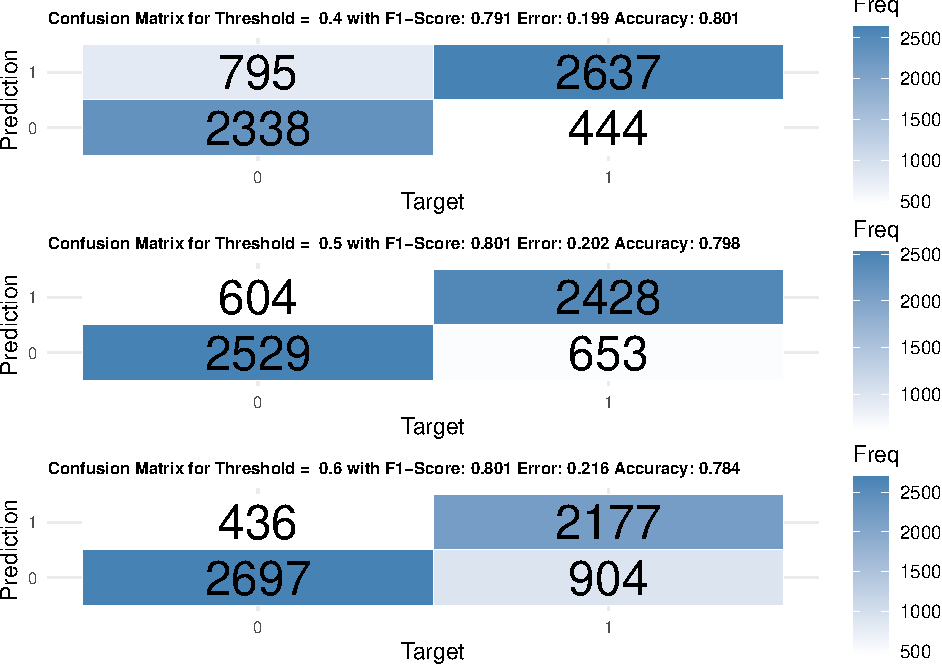
\includegraphics{Rain_Australia_files/figure-latex/selected model-1.pdf}

\hypertarget{comparison-of-3-models}{%
\subsection{Comparison of 3 Models}\label{comparison-of-3-models}}

In the following plots, we compared each of the performance metrics
previously computed across all the logistic regression models for each
prediction threshold. By observing the results, we noticed close
performance across all the models, with the simplest model before
balancing and feature selection showing a slightly higher accuracy and
F1 score, and lower error rate.

\begin{Shaded}
\begin{Highlighting}[]
\DocumentationTok{\#\# Summary Statistics: F1{-}Score, Error, Accuracy}

\NormalTok{models }\OtherTok{\textless{}{-}}
  \FunctionTok{c}\NormalTok{(}\StringTok{"Simple GLM"}\NormalTok{,}
    \StringTok{"GLM with Balancing"}\NormalTok{,}
    \StringTok{"GLM with Balancing and Feature Selection"}\NormalTok{)}
\NormalTok{model\_suffix }\OtherTok{\textless{}{-}} \FunctionTok{c}\NormalTok{(}\StringTok{"\_0"}\NormalTok{, }\StringTok{"\_balanced"}\NormalTok{, }\StringTok{""}\NormalTok{)}

\NormalTok{thresholds }\OtherTok{\textless{}{-}} \FunctionTok{c}\NormalTok{(}\DecValTok{4}\NormalTok{, }\DecValTok{5}\NormalTok{, }\DecValTok{6}\NormalTok{)}
\NormalTok{threshold\_values }\OtherTok{\textless{}{-}} \FunctionTok{c}\NormalTok{(}\FloatTok{0.4}\NormalTok{, }\FloatTok{0.5}\NormalTok{, }\FloatTok{0.6}\NormalTok{)}

\NormalTok{metrics }\OtherTok{\textless{}{-}}
  \FunctionTok{data.frame}\NormalTok{(}
    \AttributeTok{Model =} \FunctionTok{character}\NormalTok{(),}
    \AttributeTok{Threshold =} \FunctionTok{numeric}\NormalTok{(),}
    \AttributeTok{F1\_Score =} \FunctionTok{numeric}\NormalTok{(),}
    \AttributeTok{Error =} \FunctionTok{numeric}\NormalTok{(),}
    \AttributeTok{Accuracy =} \FunctionTok{numeric}\NormalTok{(),}
    \AttributeTok{stringsAsFactors =} \ConstantTok{FALSE}
\NormalTok{  )}

\NormalTok{j }\OtherTok{\textless{}{-}}  \DecValTok{1}

\ControlFlowTok{for}\NormalTok{ (model }\ControlFlowTok{in}\NormalTok{ models) \{}
\NormalTok{  model\_suff }\OtherTok{\textless{}{-}}\NormalTok{ model\_suffix[j]}
\NormalTok{  j }\OtherTok{\textless{}{-}}\NormalTok{  j }\SpecialCharTok{+} \DecValTok{1}
  \ControlFlowTok{for}\NormalTok{ (i }\ControlFlowTok{in} \DecValTok{1}\SpecialCharTok{:}\FunctionTok{length}\NormalTok{(thresholds)) \{}
\NormalTok{    threshold }\OtherTok{\textless{}{-}}\NormalTok{ thresholds[i]}
\NormalTok{    threshold\_value }\OtherTok{\textless{}{-}}\NormalTok{ threshold\_values[i]}
    
    \CommentTok{\# Calculate the F1 score for each combination of model and threshold}
\NormalTok{    cm\_name }\OtherTok{\textless{}{-}} \FunctionTok{paste0}\NormalTok{(}\StringTok{"cm"}\NormalTok{, threshold, model\_suff)}
\NormalTok{    cm }\OtherTok{\textless{}{-}} \FunctionTok{get}\NormalTok{(cm\_name)}
\NormalTok{    f1\_score }\OtherTok{\textless{}{-}}\NormalTok{ cm}\SpecialCharTok{$}\NormalTok{byClass[}\StringTok{"F1"}\NormalTok{]}
    
\NormalTok{    error\_name }\OtherTok{\textless{}{-}} \FunctionTok{paste0}\NormalTok{(}\StringTok{"error"}\NormalTok{, threshold, model\_suff)}
\NormalTok{    error }\OtherTok{\textless{}{-}} \FunctionTok{get}\NormalTok{(error\_name)}
    
\NormalTok{    accuracy\_name }\OtherTok{\textless{}{-}} \FunctionTok{paste0}\NormalTok{(}\StringTok{"accuracy"}\NormalTok{, threshold, model\_suff)}
\NormalTok{    accuracy }\OtherTok{\textless{}{-}} \FunctionTok{get}\NormalTok{(accuracy\_name)}
    
    \CommentTok{\# Add the F1 score to the data frame}
\NormalTok{    metrics }\OtherTok{\textless{}{-}}
      \FunctionTok{rbind}\NormalTok{(}
\NormalTok{        metrics,}
        \FunctionTok{data.frame}\NormalTok{(}
          \AttributeTok{Model =}\NormalTok{ model,}
          \AttributeTok{Threshold =}\NormalTok{ threshold\_value,}
          \AttributeTok{F1\_Score =}\NormalTok{ f1\_score,}
          \AttributeTok{Error =}\NormalTok{ error,}
          \AttributeTok{Accuracy =}\NormalTok{ accuracy,}
          \AttributeTok{stringsAsFactors =} \ConstantTok{FALSE}\NormalTok{,}
          \AttributeTok{row.names =} \ConstantTok{NULL}
\NormalTok{        )}
\NormalTok{      )}
\NormalTok{  \}}
\NormalTok{\}}

\FunctionTok{print}\NormalTok{(metrics)}
\end{Highlighting}
\end{Shaded}

\begin{verbatim}
##                                      Model Threshold  F1_Score     Error
## 1                               Simple GLM       0.4 0.9030458 0.1527827
## 2                               Simple GLM       0.5 0.9074894 0.1496632
## 3                               Simple GLM       0.6 0.9087790 0.1507976
## 4                       GLM with Balancing       0.4 0.7896517 0.2001931
## 5                       GLM with Balancing       0.5 0.8012678 0.2018024
## 6                       GLM with Balancing       0.6 0.8015472 0.2146765
## 7 GLM with Balancing and Feature Selection       0.4 0.7905325 0.1993885
## 8 GLM with Balancing and Feature Selection       0.5 0.8009501 0.2022852
## 9 GLM with Balancing and Feature Selection       0.6 0.8010098 0.2156421
##    Accuracy
## 1 0.8472173
## 2 0.8503368
## 3 0.8492024
## 4 0.7998069
## 5 0.7981976
## 6 0.7853235
## 7 0.8006115
## 8 0.7977148
## 9 0.7843579
\end{verbatim}

\hypertarget{visualizing-data-classifications-from-predictions}{%
\subsection{Visualizing data classifications from
predictions}\label{visualizing-data-classifications-from-predictions}}

In addition to comparing performance metrics across the three models, we
also sought to visualize the separation of classes in scatter plots
between two predictive features: Sunshine and Temp3pm. As seen for the
majority of the features, we are unable to completely separate the
classes in the scatterplots since the features are highly correlated. To
pair with these scatter plots, we created logistic curves for each of
our logistic regresison models that plot the predicted probability of
the RainTomorrow classification of samples against the true
classification. As expected, points with predicted probabilities closer
to zero are being classified as 0 for RainTomorrow, whereas points with
probabilities closer to one are being classified as 1. In comparing the
three models, the Simple GLM appears to be more skewed to the right due
to zero being the dominating class. While in the other two modified GLM
models, undersampling reduced the number of samples of the 0 class to a
point at which the classes had an equal number of samples. This likely
led to less skewing of the logistic curve, but also a more even
distribution of points around the middle of the plots, indicating less
polarity in the classification.

\begin{Shaded}
\begin{Highlighting}[]
\CommentTok{\#for different features: mintemp an temp3pm}
\NormalTok{a00 }\OtherTok{\textless{}{-}} \FunctionTok{ggplot}\NormalTok{(}\AttributeTok{data =}\NormalTok{ rain\_n\_test0 , }\FunctionTok{aes}\NormalTok{(}\AttributeTok{x =}\NormalTok{ MinTemp,}
\AttributeTok{y =}\NormalTok{ Temp3pm,}
\AttributeTok{color=} \FunctionTok{as.factor}\NormalTok{(RainTomorrow) )) }\SpecialCharTok{+}
\FunctionTok{geom\_point}\NormalTok{()}\SpecialCharTok{+}
\FunctionTok{labs}\NormalTok{(}\AttributeTok{x =} \StringTok{"Mintemp"}\NormalTok{,}
\AttributeTok{y =} \StringTok{"Temp3pm"}\NormalTok{,}
\AttributeTok{color =} \StringTok{"Rain Tomorrow"}\NormalTok{) }\SpecialCharTok{+}
\FunctionTok{theme}\NormalTok{(}\AttributeTok{legend.position =} \FunctionTok{c}\NormalTok{(}\FloatTok{0.8}\NormalTok{, }\FloatTok{0.8}\NormalTok{))}

\CommentTok{\# original classification }
\NormalTok{a0 }\OtherTok{\textless{}{-}} \FunctionTok{ggplot}\NormalTok{(}\AttributeTok{data =}\NormalTok{ rain\_n\_test0 , }\FunctionTok{aes}\NormalTok{(}\AttributeTok{x =}\NormalTok{ Sunshine,}
\AttributeTok{y =}\NormalTok{ Temp3pm,}
\AttributeTok{color=} \FunctionTok{as.factor}\NormalTok{(RainTomorrow) )) }\SpecialCharTok{+}
\FunctionTok{geom\_point}\NormalTok{()}\SpecialCharTok{+}
\FunctionTok{labs}\NormalTok{(}\AttributeTok{x =} \StringTok{"Sunshine"}\NormalTok{,}
\AttributeTok{y =} \StringTok{"Temp3pm"}\NormalTok{,}
\AttributeTok{color =} \StringTok{"Rain Tomorrow"}\NormalTok{) }\SpecialCharTok{+}
\FunctionTok{theme}\NormalTok{(}\AttributeTok{legend.position =} \FunctionTok{c}\NormalTok{(}\FloatTok{0.8}\NormalTok{, }\FloatTok{0.8}\NormalTok{))}

\CommentTok{\# Simple GLM: Threshold of 0.5}
\NormalTok{a2 }\OtherTok{\textless{}{-}} \FunctionTok{ggplot}\NormalTok{(}\AttributeTok{data =}\NormalTok{ rain\_n\_test0 , }\FunctionTok{aes}\NormalTok{(}\AttributeTok{x =}\NormalTok{ Sunshine,}
\AttributeTok{y =}\NormalTok{ Temp3pm,}
\AttributeTok{color=} \FunctionTok{as.factor}\NormalTok{(glm\_predict\_5\_0) )) }\SpecialCharTok{+}
\FunctionTok{geom\_point}\NormalTok{()}\SpecialCharTok{+}
\FunctionTok{labs}\NormalTok{(}\AttributeTok{x =} \StringTok{"Sunshine"}\NormalTok{,}
\AttributeTok{y =} \StringTok{"Temp3pm"}\NormalTok{,}
\AttributeTok{color =} \StringTok{"Rain Tomorrow"}\NormalTok{,}
\AttributeTok{title =} \StringTok{"Simple GLM: 0.5"}\NormalTok{) }\SpecialCharTok{+}
\FunctionTok{theme}\NormalTok{(}\AttributeTok{legend.position =} \FunctionTok{c}\NormalTok{(}\FloatTok{0.8}\NormalTok{, }\FloatTok{0.8}\NormalTok{))}

\CommentTok{\# GLM with Balancing: Threshold of 0.5}
\NormalTok{b2 }\OtherTok{\textless{}{-}} \FunctionTok{ggplot}\NormalTok{(}\AttributeTok{data =}\NormalTok{ rain\_balanced\_test , }\FunctionTok{aes}\NormalTok{(}\AttributeTok{x =}\NormalTok{ Sunshine,}
\AttributeTok{y =}\NormalTok{ Temp3pm,}
\AttributeTok{color=} \FunctionTok{as.factor}\NormalTok{(glm\_predict\_5\_balanced) )) }\SpecialCharTok{+}
\FunctionTok{geom\_point}\NormalTok{()}\SpecialCharTok{+}
\FunctionTok{labs}\NormalTok{(}\AttributeTok{x =} \StringTok{"Sunshine"}\NormalTok{,}
\AttributeTok{y =} \StringTok{"Temp3pm"}\NormalTok{,}
\AttributeTok{color =} \StringTok{"Rain Tomorrow"}\NormalTok{,}
\AttributeTok{title =} \StringTok{"GLM with Balancing: 0.5"}\NormalTok{) }\SpecialCharTok{+}
\FunctionTok{theme}\NormalTok{(}\AttributeTok{legend.position =} \FunctionTok{c}\NormalTok{(}\FloatTok{0.8}\NormalTok{, }\FloatTok{0.8}\NormalTok{))}

\CommentTok{\# GLM with Balancing and Feature Selection}
\NormalTok{c2 }\OtherTok{\textless{}{-}} \FunctionTok{ggplot}\NormalTok{(}\AttributeTok{data =}\NormalTok{ rain\_balanced\_test , }\FunctionTok{aes}\NormalTok{(}\AttributeTok{x =}\NormalTok{ Sunshine,}
\AttributeTok{y =}\NormalTok{ Temp3pm,}
\AttributeTok{color=} \FunctionTok{as.factor}\NormalTok{(glm\_predict\_5) )) }\SpecialCharTok{+}
\FunctionTok{geom\_point}\NormalTok{()}\SpecialCharTok{+}
\FunctionTok{labs}\NormalTok{(}\AttributeTok{x =} \StringTok{"Sunshine"}\NormalTok{,}
\AttributeTok{y =} \StringTok{"Temp3pm"}\NormalTok{,}
\AttributeTok{color =} \StringTok{"Rain Tomorrow"}\NormalTok{,}
\AttributeTok{title =} \StringTok{"GLM with Balancing and Feature Selection: 0.5"}\NormalTok{) }\SpecialCharTok{+}
\FunctionTok{theme}\NormalTok{(}\AttributeTok{legend.position =} \FunctionTok{c}\NormalTok{(}\FloatTok{0.8}\NormalTok{, }\FloatTok{0.8}\NormalTok{))}

\FunctionTok{grid.arrange}\NormalTok{(a0, a2, b2, c2, }\AttributeTok{nrow =} \DecValTok{2}\NormalTok{)}
\end{Highlighting}
\end{Shaded}

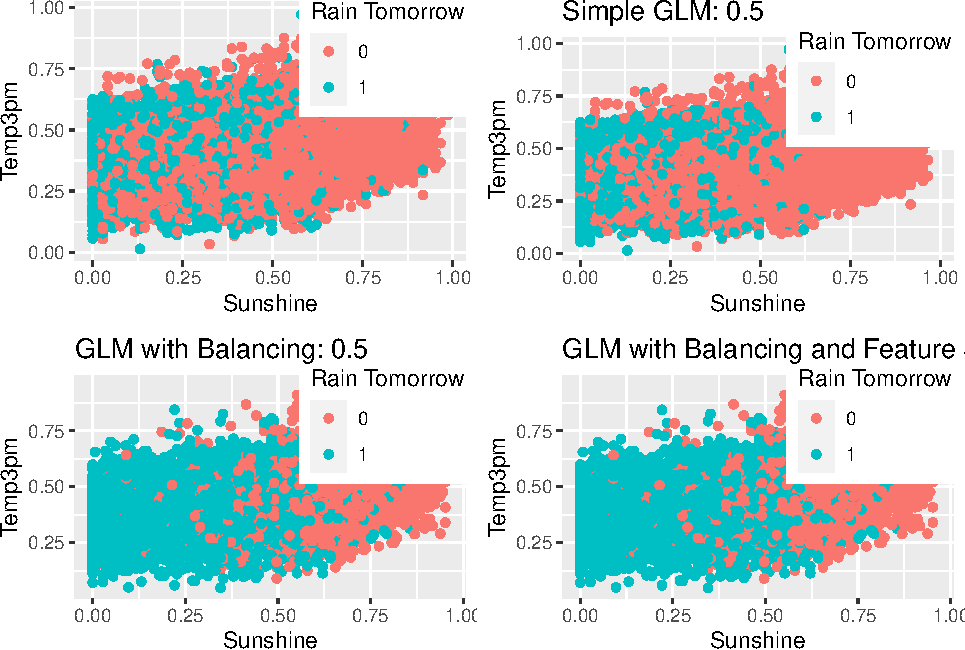
\includegraphics{Rain_Australia_files/figure-latex/Visualizing data classifications-1.pdf}

\begin{Shaded}
\begin{Highlighting}[]
\NormalTok{predicted\_data }\OtherTok{\textless{}{-}}
  \FunctionTok{data.frame}\NormalTok{(}\AttributeTok{prob\_of\_rain =}\NormalTok{ glm\_predict0,}
             \AttributeTok{RainTomorrow =}\NormalTok{ rain\_n\_test0}\SpecialCharTok{$}\NormalTok{RainTomorrow)}
\NormalTok{predicted\_data }\OtherTok{\textless{}{-}}
\NormalTok{  predicted\_data[}\FunctionTok{order}\NormalTok{(predicted\_data}\SpecialCharTok{$}\NormalTok{prob\_of\_rain, }\AttributeTok{decreasing =} \ConstantTok{FALSE}\NormalTok{), ]}
\NormalTok{predicted\_data}\SpecialCharTok{$}\NormalTok{rank }\OtherTok{\textless{}{-}}  \DecValTok{1}\SpecialCharTok{:}\FunctionTok{nrow}\NormalTok{(predicted\_data)}

\NormalTok{a3 }\OtherTok{\textless{}{-}}
  \FunctionTok{ggplot}\NormalTok{(}\AttributeTok{data =}\NormalTok{ predicted\_data, }\FunctionTok{aes}\NormalTok{(}\AttributeTok{x =}\NormalTok{ rank, }\AttributeTok{y =}\NormalTok{ prob\_of\_rain)) }\SpecialCharTok{+}
  \FunctionTok{geom\_point}\NormalTok{(}
    \FunctionTok{aes}\NormalTok{(}\AttributeTok{color =} \FunctionTok{as.factor}\NormalTok{(RainTomorrow)),}
    \AttributeTok{alpha =} \DecValTok{1}\NormalTok{,}
    \AttributeTok{shape =} \DecValTok{1}\NormalTok{,}
    \AttributeTok{stroke =} \DecValTok{1}
\NormalTok{  ) }\SpecialCharTok{+}
  \FunctionTok{xlab}\NormalTok{(}\StringTok{"Index"}\NormalTok{) }\SpecialCharTok{+}
  \FunctionTok{ylab}\NormalTok{(}\StringTok{"Predicted probability"}\NormalTok{) }\SpecialCharTok{+}
  \FunctionTok{ggtitle}\NormalTok{(}\StringTok{"Estimated Logistic Curve {-} Simple GLM"}\NormalTok{) }\SpecialCharTok{+}
  \FunctionTok{labs}\NormalTok{(}\AttributeTok{color =} \StringTok{"Rain Tomorrow"}\NormalTok{)}

\NormalTok{predicted\_data }\OtherTok{\textless{}{-}}
  \FunctionTok{data.frame}\NormalTok{(}\AttributeTok{prob\_of\_rain =}\NormalTok{ glm\_predict\_balanced,}
             \AttributeTok{RainTomorrow =}\NormalTok{ rain\_balanced\_test}\SpecialCharTok{$}\NormalTok{RainTomorrow)}
\NormalTok{predicted\_data }\OtherTok{\textless{}{-}}
\NormalTok{  predicted\_data[}\FunctionTok{order}\NormalTok{(predicted\_data}\SpecialCharTok{$}\NormalTok{prob\_of\_rain, }\AttributeTok{decreasing =} \ConstantTok{FALSE}\NormalTok{), ]}
\NormalTok{predicted\_data}\SpecialCharTok{$}\NormalTok{rank }\OtherTok{\textless{}{-}}  \DecValTok{1}\SpecialCharTok{:}\FunctionTok{nrow}\NormalTok{(predicted\_data)}

\NormalTok{b3 }\OtherTok{\textless{}{-}}
  \FunctionTok{ggplot}\NormalTok{(}\AttributeTok{data =}\NormalTok{ predicted\_data, }\FunctionTok{aes}\NormalTok{(}\AttributeTok{x =}\NormalTok{ rank, }\AttributeTok{y =}\NormalTok{ prob\_of\_rain)) }\SpecialCharTok{+}
  \FunctionTok{geom\_point}\NormalTok{(}
    \FunctionTok{aes}\NormalTok{(}\AttributeTok{color =} \FunctionTok{as.factor}\NormalTok{(RainTomorrow)),}
    \AttributeTok{alpha =} \DecValTok{1}\NormalTok{,}
    \AttributeTok{shape =} \DecValTok{1}\NormalTok{,}
    \AttributeTok{stroke =} \DecValTok{1}
\NormalTok{  ) }\SpecialCharTok{+}
  \FunctionTok{xlab}\NormalTok{(}\StringTok{"Index"}\NormalTok{) }\SpecialCharTok{+}
  \FunctionTok{ylab}\NormalTok{(}\StringTok{"Predicted probability"}\NormalTok{) }\SpecialCharTok{+}
  \FunctionTok{ggtitle}\NormalTok{(}\StringTok{"Estimated Logistic Curve {-} Simple GLM with Balancing"}\NormalTok{) }\SpecialCharTok{+}
  \FunctionTok{labs}\NormalTok{(}\AttributeTok{color =} \StringTok{"Rain Tomorrow"}\NormalTok{)}

\NormalTok{predicted\_data }\OtherTok{\textless{}{-}}
  \FunctionTok{data.frame}\NormalTok{(}\AttributeTok{prob\_of\_rain =}\NormalTok{ glm\_predict,}
             \AttributeTok{RainTomorrow =}\NormalTok{ rain\_balanced\_test}\SpecialCharTok{$}\NormalTok{RainTomorrow)}
\NormalTok{predicted\_data }\OtherTok{\textless{}{-}}
\NormalTok{  predicted\_data[}\FunctionTok{order}\NormalTok{(predicted\_data}\SpecialCharTok{$}\NormalTok{prob\_of\_rain, }\AttributeTok{decreasing =} \ConstantTok{FALSE}\NormalTok{), ]}
\NormalTok{predicted\_data}\SpecialCharTok{$}\NormalTok{rank }\OtherTok{\textless{}{-}}  \DecValTok{1}\SpecialCharTok{:}\FunctionTok{nrow}\NormalTok{(predicted\_data)}

\NormalTok{c3 }\OtherTok{\textless{}{-}}
  \FunctionTok{ggplot}\NormalTok{(}\AttributeTok{data =}\NormalTok{ predicted\_data, }\FunctionTok{aes}\NormalTok{(}\AttributeTok{x =}\NormalTok{ rank, }\AttributeTok{y =}\NormalTok{ prob\_of\_rain)) }\SpecialCharTok{+}
  \FunctionTok{geom\_point}\NormalTok{(}
    \FunctionTok{aes}\NormalTok{(}\AttributeTok{color =} \FunctionTok{as.factor}\NormalTok{(RainTomorrow)),}
    \AttributeTok{alpha =} \DecValTok{1}\NormalTok{,}
    \AttributeTok{shape =} \DecValTok{1}\NormalTok{,}
    \AttributeTok{stroke =} \DecValTok{1}
\NormalTok{  ) }\SpecialCharTok{+}
  \FunctionTok{xlab}\NormalTok{(}\StringTok{"Index"}\NormalTok{) }\SpecialCharTok{+}
  \FunctionTok{ylab}\NormalTok{(}\StringTok{"Predicted probability"}\NormalTok{) }\SpecialCharTok{+}
  \FunctionTok{ggtitle}\NormalTok{(}\StringTok{"Estimated Logistic Curve {-} Simple GLM with Balancing and Feature }
\StringTok{          Selection"}\NormalTok{) }\SpecialCharTok{+}
  \FunctionTok{labs}\NormalTok{(}\AttributeTok{color =} \StringTok{"Rain Tomorrow"}\NormalTok{)}

\FunctionTok{grid.arrange}\NormalTok{(a3, b3, c3, }\AttributeTok{nrow =} \DecValTok{3}\NormalTok{)}
\end{Highlighting}
\end{Shaded}

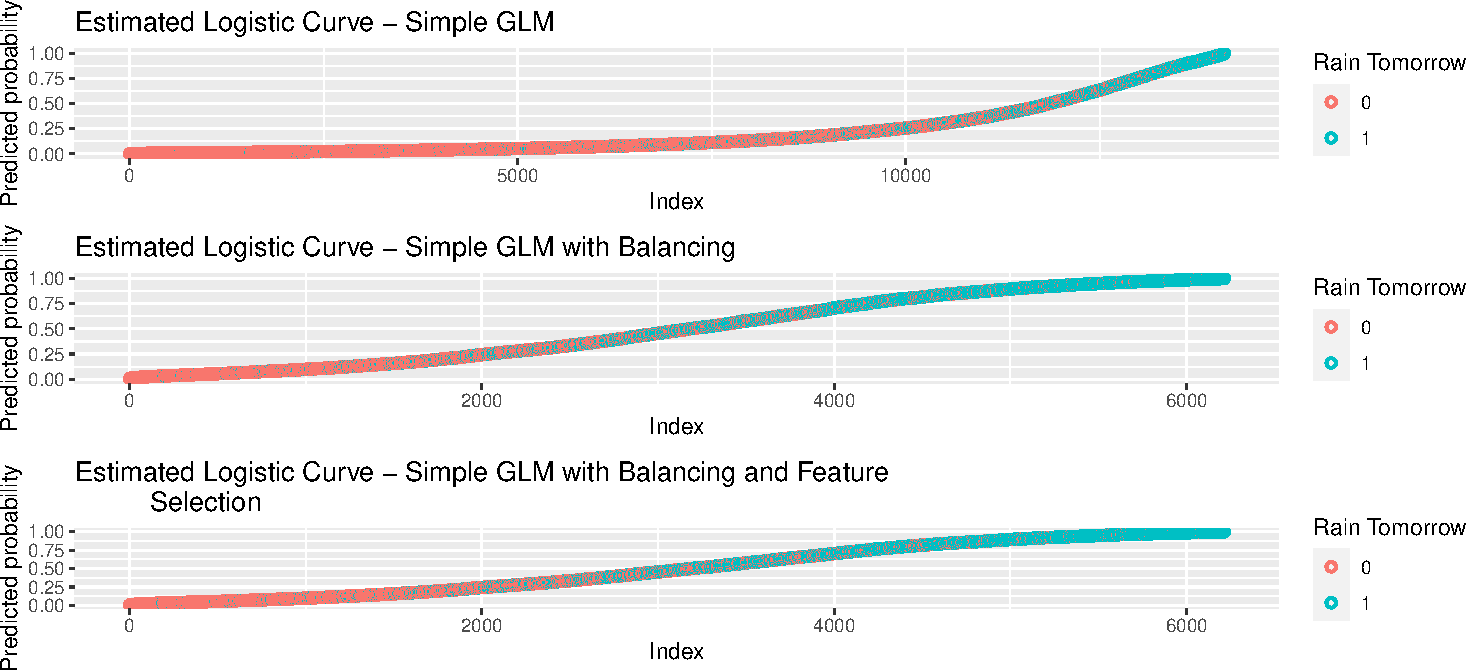
\includegraphics{Rain_Australia_files/figure-latex/logistic regression plots-1.pdf}

\begin{Shaded}
\begin{Highlighting}[]
\NormalTok{X\_train\_subset }\OtherTok{\textless{}{-}} \FunctionTok{model.matrix}\NormalTok{(RainTomorrow}\SpecialCharTok{\textasciitilde{}}\NormalTok{., }\AttributeTok{data=}\NormalTok{rain\_subset\_train)}
\NormalTok{X\_test\_subset }\OtherTok{\textless{}{-}} \FunctionTok{model.matrix}\NormalTok{(RainTomorrow}\SpecialCharTok{\textasciitilde{}}\NormalTok{., }\AttributeTok{data=}\NormalTok{rain\_subset\_test)}
\NormalTok{X\_train\_subset }\OtherTok{\textless{}{-}}\NormalTok{ X\_train\_subset[,}\SpecialCharTok{{-}}\DecValTok{1}\NormalTok{]}
\NormalTok{X\_test\_subset }\OtherTok{\textless{}{-}}\NormalTok{ X\_test\_subset[,}\SpecialCharTok{{-}}\DecValTok{1}\NormalTok{]}

\CommentTok{\# Target vector}
\NormalTok{y\_train\_subset }\OtherTok{\textless{}{-}}\NormalTok{ rain\_subset\_train}\SpecialCharTok{$}\NormalTok{RainTomorrow}
\NormalTok{y\_test\_subset }\OtherTok{\textless{}{-}}\NormalTok{ rain\_subset\_test}\SpecialCharTok{$}\NormalTok{RainTomorrow}
\end{Highlighting}
\end{Shaded}

\hypertarget{regularized-regression-models}{%
\section{Regularized Regression
Models}\label{regularized-regression-models}}

Beyond the standard logistic regression models, we chose to implement
two alternative regularization models: LASSO and Ridge Regression. Both
regularization techniques introduce a penalty team to the standard
regression model; Least Absolute Shrinkage and Selection Operator
(LASSO) regression utilizes the L1 norm, which is the sum of the
absolute value of the parameters multiplied by a hyperparamter, lambda,
whereas Ridge Regression uses the L2 norm, which is the square root of
the sum of squared parameters multiplied by the lambda hyperparameter.
The lambda hyperparameter plays a major role in determining the level of
regularization introduced in the model; the higher the lambda value is,
the higher the regularization and vice-versa. Moreover, LASSO regression
is suitable for performing another form of feature selection as it
introduces sparsity in our model and prioritizes fewer parameters. Ridge
regression, on the other hand, is effective for dealing with
multicollinearity (identified by VIF), when features are highly
correlated, by shrinking the magnitude of the coefficients. According to
the VIF calculated previously (greater than 1), our data has high
multicollinearity, which can be potentially addressed using the ridge
regression.

\hypertarget{lasso-and-ridge-balanced-wo-feature-selection}{%
\subsection{LASSO and Ridge Balanced w/o Feature
Selection}\label{lasso-and-ridge-balanced-wo-feature-selection}}

\begin{Shaded}
\begin{Highlighting}[]
\FunctionTok{set.seed}\NormalTok{(}\DecValTok{123}\NormalTok{)}

\CommentTok{\#We\textquotesingle{}re first implementing lasso/ridge with balanced data with no feature }
\CommentTok{\#selection}

\NormalTok{X }\OtherTok{\textless{}{-}} \FunctionTok{model.matrix}\NormalTok{(RainTomorrow }\SpecialCharTok{\textasciitilde{}}\NormalTok{ ., }\AttributeTok{data =}\NormalTok{ rain\_balanced)}
\NormalTok{X }\OtherTok{\textless{}{-}}\NormalTok{ X[, }\SpecialCharTok{{-}}\DecValTok{1}\NormalTok{]}

\NormalTok{X\_train }\OtherTok{\textless{}{-}} \FunctionTok{model.matrix}\NormalTok{(RainTomorrow }\SpecialCharTok{\textasciitilde{}}\NormalTok{ ., }\AttributeTok{data =}\NormalTok{ rain\_balanced\_train)}
\NormalTok{X\_test }\OtherTok{\textless{}{-}} \FunctionTok{model.matrix}\NormalTok{(RainTomorrow }\SpecialCharTok{\textasciitilde{}}\NormalTok{ ., }\AttributeTok{data =}\NormalTok{ rain\_balanced\_test)}
\NormalTok{X\_train }\OtherTok{\textless{}{-}}\NormalTok{ X\_train[, }\SpecialCharTok{{-}}\DecValTok{1}\NormalTok{]}
\NormalTok{X\_test }\OtherTok{\textless{}{-}}\NormalTok{ X\_test[, }\SpecialCharTok{{-}}\DecValTok{1}\NormalTok{]}

\CommentTok{\# Target vector}
\NormalTok{y }\OtherTok{\textless{}{-}}\NormalTok{ rain\_balanced}\SpecialCharTok{$}\NormalTok{RainTomorrow}
\NormalTok{y\_train }\OtherTok{\textless{}{-}}\NormalTok{ rain\_balanced\_train}\SpecialCharTok{$}\NormalTok{RainTomorrow}
\NormalTok{y\_test }\OtherTok{\textless{}{-}}\NormalTok{ rain\_balanced\_test}\SpecialCharTok{$}\NormalTok{RainTomorrow}

\CommentTok{\# alpha=0 for ridge, alpha=1 (default) for lasso}

\CommentTok{\# Ridge Regression (L2)}

\NormalTok{ridge\_cv }\OtherTok{\textless{}{-}}
  \FunctionTok{cv.glmnet}\NormalTok{(}
\NormalTok{    X\_train,}
\NormalTok{    y\_train,}
    \AttributeTok{alpha =} \DecValTok{0}\NormalTok{,}
    \AttributeTok{family =} \StringTok{"binomial"}\NormalTok{,}
    \AttributeTok{type.measure =} \StringTok{"class"}
\NormalTok{  )}
\FunctionTok{plot}\NormalTok{(ridge\_cv)}
\end{Highlighting}
\end{Shaded}

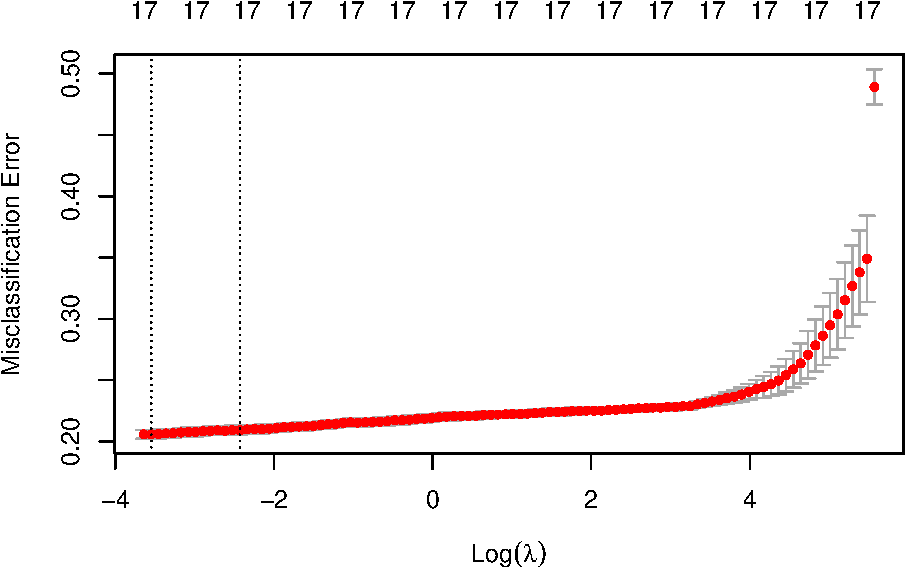
\includegraphics{Rain_Australia_files/figure-latex/unnamed-chunk-1-1.pdf}

\begin{Shaded}
\begin{Highlighting}[]
\CommentTok{\# To select best lambda}
\NormalTok{lambda\_opt\_ridge }\OtherTok{\textless{}{-}}\NormalTok{ ridge\_cv}\SpecialCharTok{$}\NormalTok{lambda.min}
\NormalTok{lambda\_opt\_ridge}
\end{Highlighting}
\end{Shaded}

\begin{verbatim}
## [1] 0.0288348
\end{verbatim}

\begin{Shaded}
\begin{Highlighting}[]
\NormalTok{pred\_ridge }\OtherTok{\textless{}{-}}
  \FunctionTok{predict}\NormalTok{(ridge\_cv, X\_test, }\AttributeTok{type =} \StringTok{"class"}\NormalTok{, }\AttributeTok{s =}\NormalTok{ lambda\_opt\_ridge)}
\NormalTok{error\_ridge }\OtherTok{\textless{}{-}} \FunctionTok{mean}\NormalTok{(pred\_ridge }\SpecialCharTok{!=}\NormalTok{ y\_test) }\CommentTok{\# 0.2133891}
\NormalTok{accuracy\_ridge }\OtherTok{\textless{}{-}} \FunctionTok{mean}\NormalTok{(pred\_ridge }\SpecialCharTok{==}\NormalTok{ y\_test) }\CommentTok{\# 0.7866109}
\NormalTok{cm\_ridge }\OtherTok{\textless{}{-}}
  \FunctionTok{confusionMatrix}\NormalTok{(}
    \AttributeTok{data =} \FunctionTok{factor}\NormalTok{(pred\_ridge),}
    \AttributeTok{reference =} \FunctionTok{factor}\NormalTok{(y\_test),}
    \AttributeTok{mode =} \StringTok{\textquotesingle{}everything\textquotesingle{}}
\NormalTok{  ) }\CommentTok{\# F1 : 0.7856}

\CommentTok{\#Lasso Regression (L1)}
\NormalTok{lasso\_cv }\OtherTok{\textless{}{-}}
  \FunctionTok{cv.glmnet}\NormalTok{(}
\NormalTok{    X\_train,}
\NormalTok{    y\_train,}
    \AttributeTok{alpha =} \DecValTok{1}\NormalTok{,}
    \AttributeTok{family =} \StringTok{"binomial"}\NormalTok{,}
    \AttributeTok{type.measure =} \StringTok{"class"}
\NormalTok{  )}
\FunctionTok{plot}\NormalTok{(lasso\_cv)}
\end{Highlighting}
\end{Shaded}

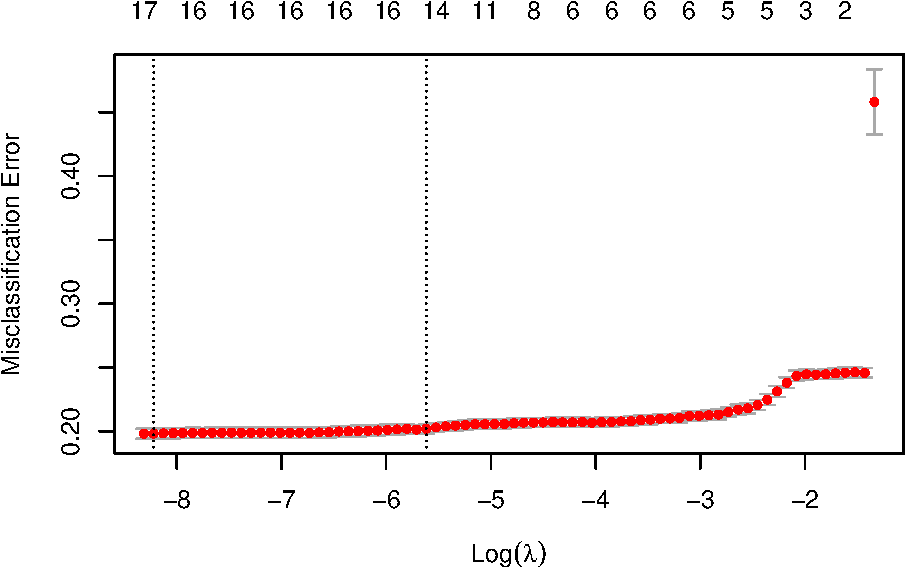
\includegraphics{Rain_Australia_files/figure-latex/unnamed-chunk-1-2.pdf}

\begin{Shaded}
\begin{Highlighting}[]
\NormalTok{lambda\_opt\_lasso }\OtherTok{\textless{}{-}}\NormalTok{ lasso\_cv}\SpecialCharTok{$}\NormalTok{lambda.min}
\NormalTok{lambda\_opt\_lasso}
\end{Highlighting}
\end{Shaded}

\begin{verbatim}
## [1] 0.0002689143
\end{verbatim}

\begin{Shaded}
\begin{Highlighting}[]
\NormalTok{pred\_lasso }\OtherTok{\textless{}{-}}
  \FunctionTok{predict}\NormalTok{(lasso\_cv, X\_test, }\AttributeTok{type =} \StringTok{"class"}\NormalTok{, }\AttributeTok{s =}\NormalTok{ lambda\_opt\_lasso)}
\NormalTok{error\_lasso }\OtherTok{\textless{}{-}} \FunctionTok{mean}\NormalTok{(pred\_lasso }\SpecialCharTok{!=}\NormalTok{ y\_test) }\CommentTok{\# 0.2046991}
\NormalTok{accuracy\_lasso }\OtherTok{\textless{}{-}} \FunctionTok{mean}\NormalTok{(pred\_lasso }\SpecialCharTok{==}\NormalTok{ y\_test) }\CommentTok{\#  0.7953009}
\NormalTok{cm\_lasso }\OtherTok{\textless{}{-}}
  \FunctionTok{confusionMatrix}\NormalTok{(}
    \AttributeTok{data =} \FunctionTok{factor}\NormalTok{(pred\_lasso),}
    \AttributeTok{reference =} \FunctionTok{factor}\NormalTok{(y\_test),}
    \AttributeTok{mode =} \StringTok{\textquotesingle{}everything\textquotesingle{}}
\NormalTok{  ) }\CommentTok{\# F1 : 0.7956}
\end{Highlighting}
\end{Shaded}

\hypertarget{lasso-and-ridge-balanced-w-feature-selection}{%
\subsection{LASSO and Ridge Balanced w/ Feature
Selection}\label{lasso-and-ridge-balanced-w-feature-selection}}

\begin{Shaded}
\begin{Highlighting}[]
\CommentTok{\#Then, we implemented Ridge and LASSO after feature selection}

\CommentTok{\# Ridge Regression (L2)}

\NormalTok{ridge\_cv\_subset }\OtherTok{\textless{}{-}}
  \FunctionTok{cv.glmnet}\NormalTok{(}
\NormalTok{    X\_train\_subset,}
\NormalTok{    y\_train\_subset,}
    \AttributeTok{alpha =} \DecValTok{0}\NormalTok{,}
    \AttributeTok{family =} \StringTok{"binomial"}\NormalTok{,}
    \AttributeTok{type.measure =} \StringTok{"class"}
\NormalTok{  )}
\FunctionTok{plot}\NormalTok{(ridge\_cv\_subset)}
\end{Highlighting}
\end{Shaded}

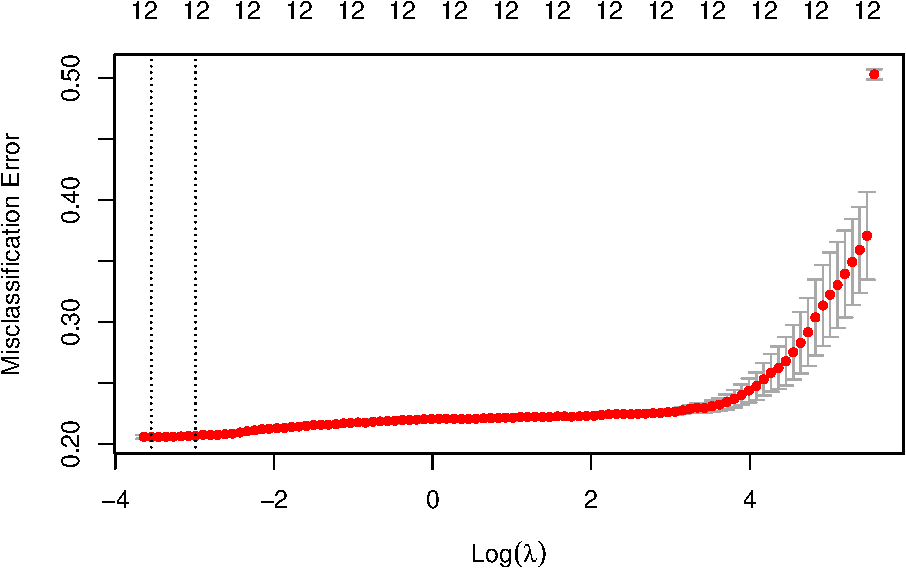
\includegraphics{Rain_Australia_files/figure-latex/unnamed-chunk-2-1.pdf}

\begin{Shaded}
\begin{Highlighting}[]
\CommentTok{\# To select best lambda}
\NormalTok{lambda\_opt\_ridge\_subset }\OtherTok{\textless{}{-}}\NormalTok{ ridge\_cv\_subset}\SpecialCharTok{$}\NormalTok{lambda.min}
\NormalTok{lambda\_opt\_ridge\_subset}
\end{Highlighting}
\end{Shaded}

\begin{verbatim}
## [1] 0.0288348
\end{verbatim}

\begin{Shaded}
\begin{Highlighting}[]
\NormalTok{pred\_ridge\_subset }\OtherTok{\textless{}{-}}
  \FunctionTok{predict}\NormalTok{(ridge\_cv\_subset, X\_test\_subset, }\AttributeTok{type =} \StringTok{"class"}\NormalTok{, }
          \AttributeTok{s =}\NormalTok{ lambda\_opt\_ridge\_subset)}
\NormalTok{error\_ridge\_subset }\OtherTok{\textless{}{-}}
  \FunctionTok{mean}\NormalTok{(pred\_ridge\_subset }\SpecialCharTok{!=}\NormalTok{ y\_test\_subset) }\CommentTok{\# 0.2125845}
\NormalTok{accuracy\_ridge\_subset }\OtherTok{\textless{}{-}}
  \FunctionTok{mean}\NormalTok{(pred\_ridge\_subset }\SpecialCharTok{==}\NormalTok{ y\_test\_subset) }\CommentTok{\# 0.7874155}
\NormalTok{cm\_ridge\_subset }\OtherTok{\textless{}{-}}
  \FunctionTok{confusionMatrix}\NormalTok{(}
    \AttributeTok{data =} \FunctionTok{factor}\NormalTok{(pred\_ridge\_subset),}
    \AttributeTok{reference =} \FunctionTok{factor}\NormalTok{(y\_test),}
    \AttributeTok{mode =} \StringTok{\textquotesingle{}everything\textquotesingle{}}
\NormalTok{  ) }\CommentTok{\# F1 : 0.7864}

\CommentTok{\#Lasso Regression (L1)}
\NormalTok{lasso\_cv\_subset }\OtherTok{\textless{}{-}}
  \FunctionTok{cv.glmnet}\NormalTok{(}
\NormalTok{    X\_train\_subset,}
\NormalTok{    y\_train\_subset,}
    \AttributeTok{alpha =} \DecValTok{1}\NormalTok{,}
    \AttributeTok{family =} \StringTok{"binomial"}\NormalTok{,}
    \AttributeTok{type.measure =} \StringTok{"class"}
\NormalTok{  )}
\FunctionTok{plot}\NormalTok{(lasso\_cv\_subset)}
\end{Highlighting}
\end{Shaded}

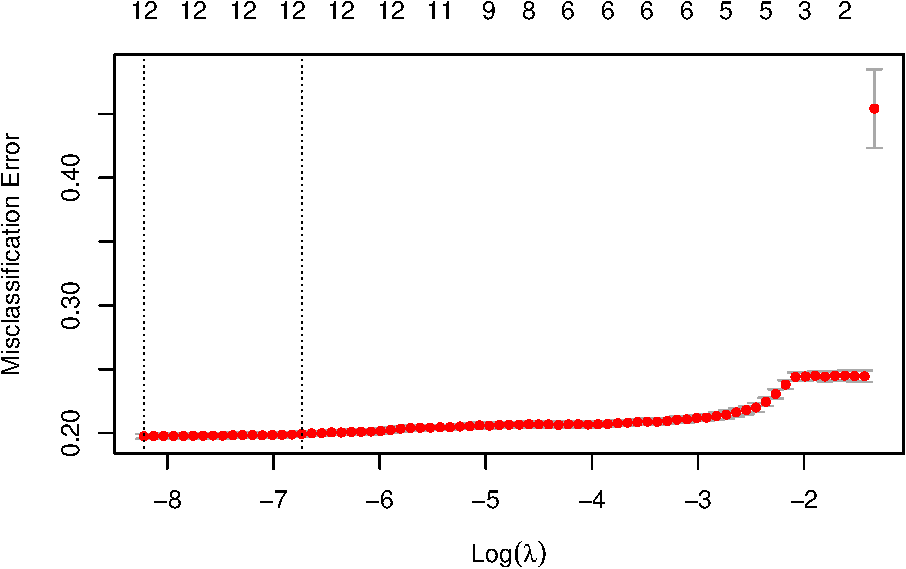
\includegraphics{Rain_Australia_files/figure-latex/unnamed-chunk-2-2.pdf}

\begin{Shaded}
\begin{Highlighting}[]
\NormalTok{lambda\_opt\_lasso\_subset }\OtherTok{\textless{}{-}}\NormalTok{ lasso\_cv\_subset}\SpecialCharTok{$}\NormalTok{lambda.min}
\NormalTok{lambda\_opt\_lasso\_subset}
\end{Highlighting}
\end{Shaded}

\begin{verbatim}
## [1] 0.0002689143
\end{verbatim}

\begin{Shaded}
\begin{Highlighting}[]
\NormalTok{pred\_lasso\_subset }\OtherTok{\textless{}{-}}
  \FunctionTok{predict}\NormalTok{(lasso\_cv\_subset, X\_test\_subset, }\AttributeTok{type =} \StringTok{"class"}\NormalTok{, }
          \AttributeTok{s =}\NormalTok{ lambda\_opt\_lasso\_subset)}
\NormalTok{error\_lasso\_subset }\OtherTok{\textless{}{-}}
  \FunctionTok{mean}\NormalTok{(pred\_lasso\_subset }\SpecialCharTok{!=}\NormalTok{ y\_test\_subset) }\CommentTok{\# 0.2059865}
\NormalTok{accuracy\_lasso\_subset }\OtherTok{\textless{}{-}}
  \FunctionTok{mean}\NormalTok{(pred\_lasso\_subset }\SpecialCharTok{==}\NormalTok{ y\_test\_subset) }\CommentTok{\# 0.7940135}
\NormalTok{cm\_lasso\_subset }\OtherTok{\textless{}{-}}
  \FunctionTok{confusionMatrix}\NormalTok{(}
    \AttributeTok{data =} \FunctionTok{factor}\NormalTok{(pred\_lasso\_subset),}
    \AttributeTok{reference =} \FunctionTok{factor}\NormalTok{(y\_test),}
    \AttributeTok{mode =} \StringTok{\textquotesingle{}everything\textquotesingle{}}
\NormalTok{  ) }\CommentTok{\# F1 : 0.7941}
\end{Highlighting}
\end{Shaded}

\hypertarget{linear-and-quadratic-discriminant-analysis}{%
\section{Linear and Quadratic Discriminant
Analysis}\label{linear-and-quadratic-discriminant-analysis}}

Linear and Quadratic Discriminant Analysis, also known as LDA and QDA,
fall into another class of statistical modeling techniques that can be
used in supervised learning. LDA projects high-dimensional data into a
lower-dimensional space while still preserving the original
classifications of the training set. The reducing technique separates
the data linearly to deduce a linear combination of the features that
best generalize the data. LDA is best suited for data with clear spatial
separation of classes and assumes the equality of covariance matrices
between the classes. Meanwhile, QDA is an extension of LDA that can
capture non-linear relationships across model features. Unlike LDA, QDA
is still suitable when the classes have unique covariance matrices. In
our project, we performed both LDA and QDA on our balanced and feature
selected data. However, since LDA and QDA are sensitive to outliers, we
performed outlier removal prior to running the models.

\hypertarget{remove-outliers-from-data}{%
\subsection{Remove outliers from data}\label{remove-outliers-from-data}}

\begin{Shaded}
\begin{Highlighting}[]
\CommentTok{\#looking for outliers in our data after balancing and feature selection }

\NormalTok{g1}\OtherTok{\textless{}{-}} \FunctionTok{ggplot}\NormalTok{(}\AttributeTok{data =}\NormalTok{ rain\_subset\_train, }\FunctionTok{aes}\NormalTok{(}\AttributeTok{y =}\NormalTok{ MinTemp,}\AttributeTok{fill =} \DecValTok{2}\NormalTok{)) }\SpecialCharTok{+}
\FunctionTok{geom\_boxplot}\NormalTok{(}\AttributeTok{outlier.colour =} \StringTok{"red"}\NormalTok{, }\AttributeTok{outlier.shape =} \DecValTok{16}\NormalTok{,}
\AttributeTok{outlier.size =} \DecValTok{2}\NormalTok{)}\SpecialCharTok{+}
\FunctionTok{theme}\NormalTok{(}\AttributeTok{legend.position=}\StringTok{"none"}\NormalTok{) }\SpecialCharTok{+}
\FunctionTok{ylab}\NormalTok{(}\StringTok{"Min Temperature"}\NormalTok{)}
\FunctionTok{chisq.out.test}\NormalTok{(rain\_subset\_train}\SpecialCharTok{$}\NormalTok{MinTemp)  }\CommentTok{\#p{-}value = 0.00151, remove 376}
\end{Highlighting}
\end{Shaded}

\begin{verbatim}
## 
##  chi-squared test for outlier
## 
## data:  rain_subset_train$MinTemp
## X-squared = 10.066, p-value = 0.00151
## alternative hypothesis: lowest value 0 is an outlier
\end{verbatim}

\begin{Shaded}
\begin{Highlighting}[]
\FunctionTok{which}\NormalTok{(rain\_subset\_train}\SpecialCharTok{$}\NormalTok{MinTemp }\SpecialCharTok{==} \DecValTok{0}\NormalTok{) }
\end{Highlighting}
\end{Shaded}

\begin{verbatim}
## [1] 376
\end{verbatim}

\begin{Shaded}
\begin{Highlighting}[]
\NormalTok{g2}\OtherTok{\textless{}{-}} \FunctionTok{ggplot}\NormalTok{(}\AttributeTok{data =}\NormalTok{ rain\_subset\_train, }\FunctionTok{aes}\NormalTok{(}\AttributeTok{y =}\NormalTok{ Sunshine,}\AttributeTok{fill =} \DecValTok{2}\NormalTok{)) }\SpecialCharTok{+}
\FunctionTok{geom\_boxplot}\NormalTok{(}\AttributeTok{outlier.colour =} \StringTok{"red"}\NormalTok{, }\AttributeTok{outlier.shape =} \DecValTok{16}\NormalTok{,}
\AttributeTok{outlier.size =} \DecValTok{2}\NormalTok{)}\SpecialCharTok{+}
\FunctionTok{theme}\NormalTok{(}\AttributeTok{legend.position=}\StringTok{"none"}\NormalTok{) }\SpecialCharTok{+}
\FunctionTok{ylab}\NormalTok{(}\StringTok{"Sunshine"}\NormalTok{)}
\FunctionTok{chisq.out.test}\NormalTok{(rain\_subset\_train}\SpecialCharTok{$}\NormalTok{Sunshine)  }\CommentTok{\#p{-}value = 0.04431, index 6965 }
\end{Highlighting}
\end{Shaded}

\begin{verbatim}
## 
##  chi-squared test for outlier
## 
## data:  rain_subset_train$Sunshine
## X-squared = 4.0448, p-value = 0.04431
## alternative hypothesis: highest value 1 is an outlier
\end{verbatim}

\begin{Shaded}
\begin{Highlighting}[]
\FunctionTok{which}\NormalTok{(rain\_subset\_train}\SpecialCharTok{$}\NormalTok{Sunshine }\SpecialCharTok{==} \DecValTok{1}\NormalTok{) }
\end{Highlighting}
\end{Shaded}

\begin{verbatim}
## [1] 6965
\end{verbatim}

\begin{Shaded}
\begin{Highlighting}[]
\NormalTok{g3}\OtherTok{\textless{}{-}} \FunctionTok{ggplot}\NormalTok{(}\AttributeTok{data =}\NormalTok{ rain\_subset\_train, }\FunctionTok{aes}\NormalTok{(}\AttributeTok{y =}\NormalTok{ WindGustSpeed,}\AttributeTok{fill =} \DecValTok{2}\NormalTok{)) }\SpecialCharTok{+}
\FunctionTok{geom\_boxplot}\NormalTok{(}\AttributeTok{outlier.colour =} \StringTok{"red"}\NormalTok{, }\AttributeTok{outlier.shape =} \DecValTok{16}\NormalTok{,}
\AttributeTok{outlier.size =} \DecValTok{2}\NormalTok{)}\SpecialCharTok{+}
\FunctionTok{theme}\NormalTok{(}\AttributeTok{legend.position=}\StringTok{"none"}\NormalTok{) }\SpecialCharTok{+}
\FunctionTok{ylab}\NormalTok{(}\StringTok{"WindGustSpeed"}\NormalTok{)}
\FunctionTok{chisq.out.test}\NormalTok{(rain\_subset\_train}\SpecialCharTok{$}\NormalTok{WindGustSpeed) }\CommentTok{\#p{-}value = 3.071e{-}07, no values }
\end{Highlighting}
\end{Shaded}

\begin{verbatim}
## 
##  chi-squared test for outlier
## 
## data:  rain_subset_train$WindGustSpeed
## X-squared = 26.204, p-value = 3.071e-07
## alternative hypothesis: highest value 0.939130434782609 is an outlier
\end{verbatim}

\begin{Shaded}
\begin{Highlighting}[]
\FunctionTok{which}\NormalTok{(rain\_subset\_train}\SpecialCharTok{$}\NormalTok{WindGustSpeed }\SpecialCharTok{==} \FloatTok{0.939130434782609}\NormalTok{) }
\end{Highlighting}
\end{Shaded}

\begin{verbatim}
## integer(0)
\end{verbatim}

\begin{Shaded}
\begin{Highlighting}[]
\NormalTok{g4}\OtherTok{\textless{}{-}} \FunctionTok{ggplot}\NormalTok{(}\AttributeTok{data =}\NormalTok{ rain\_subset\_train, }\FunctionTok{aes}\NormalTok{(}\AttributeTok{y =}\NormalTok{ WindSpeed9am,}\AttributeTok{fill =} \DecValTok{2}\NormalTok{)) }\SpecialCharTok{+}
\FunctionTok{geom\_boxplot}\NormalTok{(}\AttributeTok{outlier.colour =} \StringTok{"red"}\NormalTok{, }\AttributeTok{outlier.shape =} \DecValTok{16}\NormalTok{,}
\AttributeTok{outlier.size =} \DecValTok{2}\NormalTok{)}\SpecialCharTok{+}
\FunctionTok{theme}\NormalTok{(}\AttributeTok{legend.position=}\StringTok{"none"}\NormalTok{) }\SpecialCharTok{+}
\FunctionTok{ylab}\NormalTok{(}\StringTok{"WindSpeed9am"}\NormalTok{)}
\FunctionTok{chisq.out.test}\NormalTok{(rain\_subset\_train}\SpecialCharTok{$}\NormalTok{WindSpeed9am)  }\CommentTok{\#p{-}value = 1.43e{-}08 , no values}
\end{Highlighting}
\end{Shaded}

\begin{verbatim}
## 
##  chi-squared test for outlier
## 
## data:  rain_subset_train$WindSpeed9am
## X-squared = 32.146, p-value = 1.43e-08
## alternative hypothesis: highest value 0.969230769230769 is an outlier
\end{verbatim}

\begin{Shaded}
\begin{Highlighting}[]
\FunctionTok{which}\NormalTok{(rain\_subset\_train}\SpecialCharTok{$}\NormalTok{WindSpeed9am }\SpecialCharTok{==} \FloatTok{0.969230769230769}\NormalTok{) }
\end{Highlighting}
\end{Shaded}

\begin{verbatim}
## integer(0)
\end{verbatim}

\begin{Shaded}
\begin{Highlighting}[]
\NormalTok{g5}\OtherTok{\textless{}{-}} \FunctionTok{ggplot}\NormalTok{(}\AttributeTok{data =}\NormalTok{ rain\_subset\_train, }\FunctionTok{aes}\NormalTok{(}\AttributeTok{y =}\NormalTok{ WindSpeed3pm,}\AttributeTok{fill =} \DecValTok{2}\NormalTok{)) }\SpecialCharTok{+}
\FunctionTok{geom\_boxplot}\NormalTok{(}\AttributeTok{outlier.colour =} \StringTok{"red"}\NormalTok{, }\AttributeTok{outlier.shape =} \DecValTok{16}\NormalTok{,}
\AttributeTok{outlier.size =} \DecValTok{2}\NormalTok{)}\SpecialCharTok{+}
\FunctionTok{theme}\NormalTok{(}\AttributeTok{legend.position=}\StringTok{"none"}\NormalTok{) }\SpecialCharTok{+}
\FunctionTok{ylab}\NormalTok{(}\StringTok{"WindSpeed3pm"}\NormalTok{)}
\FunctionTok{chisq.out.test}\NormalTok{(rain\_subset\_train}\SpecialCharTok{$}\NormalTok{WindSpeed3pm)  }\CommentTok{\#p{-}value = 4.733e{-}07 , no values}
\end{Highlighting}
\end{Shaded}

\begin{verbatim}
## 
##  chi-squared test for outlier
## 
## data:  rain_subset_train$WindSpeed3pm
## X-squared = 25.37, p-value = 4.733e-07
## alternative hypothesis: highest value 0.851351351351351 is an outlier
\end{verbatim}

\begin{Shaded}
\begin{Highlighting}[]
\FunctionTok{which}\NormalTok{(rain\_subset\_train}\SpecialCharTok{$}\NormalTok{WindSpeed3pm }\SpecialCharTok{==} \FloatTok{0.851351351351351}\NormalTok{) }
\end{Highlighting}
\end{Shaded}

\begin{verbatim}
## integer(0)
\end{verbatim}

\begin{Shaded}
\begin{Highlighting}[]
\NormalTok{g6}\OtherTok{\textless{}{-}} \FunctionTok{ggplot}\NormalTok{(}\AttributeTok{data =}\NormalTok{ rain\_subset\_train, }\FunctionTok{aes}\NormalTok{(}\AttributeTok{y =}\NormalTok{ Humidity3pm,}\AttributeTok{fill =} \DecValTok{2}\NormalTok{)) }\SpecialCharTok{+}
\FunctionTok{geom\_boxplot}\NormalTok{(}\AttributeTok{outlier.colour =} \StringTok{"red"}\NormalTok{, }\AttributeTok{outlier.shape =} \DecValTok{16}\NormalTok{,}
\AttributeTok{outlier.size =} \DecValTok{2}\NormalTok{)}\SpecialCharTok{+}
\FunctionTok{theme}\NormalTok{(}\AttributeTok{legend.position=}\StringTok{"none"}\NormalTok{) }\SpecialCharTok{+}
\FunctionTok{ylab}\NormalTok{(}\StringTok{"Humidity3pm"}\NormalTok{)}
\FunctionTok{chisq.out.test}\NormalTok{(rain\_subset\_train}\SpecialCharTok{$}\NormalTok{Humidity3pm) }
\end{Highlighting}
\end{Shaded}

\begin{verbatim}
## 
##  chi-squared test for outlier
## 
## data:  rain_subset_train$Humidity3pm
## X-squared = 6.6737, p-value = 0.009785
## alternative hypothesis: lowest value 0.01 is an outlier
\end{verbatim}

\begin{Shaded}
\begin{Highlighting}[]
\CommentTok{\#p{-}value = 0.009785, \#indices:3782 10189 10959 15362 16105 18240}
\FunctionTok{which}\NormalTok{(rain\_subset\_train}\SpecialCharTok{$}\NormalTok{Humidity3pm }\SpecialCharTok{==}\FloatTok{0.01}\NormalTok{)}
\end{Highlighting}
\end{Shaded}

\begin{verbatim}
## [1]  3782 10189 10959 15362 16105 18240
\end{verbatim}

\begin{Shaded}
\begin{Highlighting}[]
\NormalTok{g7}\OtherTok{\textless{}{-}} \FunctionTok{ggplot}\NormalTok{(}\AttributeTok{data =}\NormalTok{ rain\_subset\_train, }\FunctionTok{aes}\NormalTok{(}\AttributeTok{y =}\NormalTok{ Pressure9am,}\AttributeTok{fill =} \DecValTok{2}\NormalTok{)) }\SpecialCharTok{+}
\FunctionTok{geom\_boxplot}\NormalTok{(}\AttributeTok{outlier.colour =} \StringTok{"red"}\NormalTok{, }\AttributeTok{outlier.shape =} \DecValTok{16}\NormalTok{,}
\AttributeTok{outlier.size =} \DecValTok{2}\NormalTok{)}\SpecialCharTok{+}
\FunctionTok{theme}\NormalTok{(}\AttributeTok{legend.position=}\StringTok{"none"}\NormalTok{) }\SpecialCharTok{+}
\FunctionTok{ylab}\NormalTok{(}\StringTok{"Pressure9am"}\NormalTok{)}
\FunctionTok{chisq.out.test}\NormalTok{(rain\_subset\_train}\SpecialCharTok{$}\NormalTok{Pressure9am) }\CommentTok{\# p{-}value = 2.435e{-}06, index= 1935}
\end{Highlighting}
\end{Shaded}

\begin{verbatim}
## 
##  chi-squared test for outlier
## 
## data:  rain_subset_train$Pressure9am
## X-squared = 22.217, p-value = 2.435e-06
## alternative hypothesis: lowest value 0.0283806343906518 is an outlier
\end{verbatim}

\begin{Shaded}
\begin{Highlighting}[]
\FunctionTok{which}\NormalTok{(rain\_subset\_train}\SpecialCharTok{$}\NormalTok{Pressure9am }\SpecialCharTok{==}\FloatTok{0.0283806343906518}\NormalTok{)}
\end{Highlighting}
\end{Shaded}

\begin{verbatim}
## [1] 1935
\end{verbatim}

\begin{Shaded}
\begin{Highlighting}[]
\NormalTok{g8}\OtherTok{\textless{}{-}} \FunctionTok{ggplot}\NormalTok{(}\AttributeTok{data =}\NormalTok{ rain\_subset\_train, }\FunctionTok{aes}\NormalTok{(}\AttributeTok{y =}\NormalTok{ Pressure3pm,}\AttributeTok{fill =} \DecValTok{2}\NormalTok{)) }\SpecialCharTok{+}
\FunctionTok{geom\_boxplot}\NormalTok{(}\AttributeTok{outlier.colour =} \StringTok{"red"}\NormalTok{, }\AttributeTok{outlier.shape =} \DecValTok{16}\NormalTok{,}
\AttributeTok{outlier.size =} \DecValTok{2}\NormalTok{)}\SpecialCharTok{+}
\FunctionTok{theme}\NormalTok{(}\AttributeTok{legend.position=}\StringTok{"none"}\NormalTok{) }\SpecialCharTok{+}
\FunctionTok{ylab}\NormalTok{(}\StringTok{"Pressure3pm"}\NormalTok{)}
\FunctionTok{chisq.out.test}\NormalTok{(rain\_subset\_train}\SpecialCharTok{$}\NormalTok{Pressure3pm)  }\CommentTok{\# p{-}value = 2.756e{-}07, index=15369}
\end{Highlighting}
\end{Shaded}

\begin{verbatim}
## 
##  chi-squared test for outlier
## 
## data:  rain_subset_train$Pressure3pm
## X-squared = 26.413, p-value = 2.756e-07
## alternative hypothesis: lowest value 0 is an outlier
\end{verbatim}

\begin{Shaded}
\begin{Highlighting}[]
\FunctionTok{which}\NormalTok{(rain\_subset\_train}\SpecialCharTok{$}\NormalTok{Pressure3pm }\SpecialCharTok{==}\DecValTok{0}\NormalTok{)}
\end{Highlighting}
\end{Shaded}

\begin{verbatim}
## [1] 15369
\end{verbatim}

\begin{Shaded}
\begin{Highlighting}[]
\NormalTok{g9}\OtherTok{\textless{}{-}} \FunctionTok{ggplot}\NormalTok{(}\AttributeTok{data =}\NormalTok{ rain\_subset\_train, }\FunctionTok{aes}\NormalTok{(}\AttributeTok{y =}\NormalTok{ Cloud9am,}\AttributeTok{fill =} \DecValTok{2}\NormalTok{)) }\SpecialCharTok{+}
\FunctionTok{geom\_boxplot}\NormalTok{(}\AttributeTok{outlier.colour =} \StringTok{"red"}\NormalTok{, }\AttributeTok{outlier.shape =} \DecValTok{16}\NormalTok{,}
\AttributeTok{outlier.size =} \DecValTok{2}\NormalTok{)}\SpecialCharTok{+}
\FunctionTok{theme}\NormalTok{(}\AttributeTok{legend.position=}\StringTok{"none"}\NormalTok{) }\SpecialCharTok{+}
\FunctionTok{ylab}\NormalTok{(}\StringTok{"Cloud9am"}\NormalTok{)}
\FunctionTok{chisq.out.test}\NormalTok{(rain\_subset\_train}\SpecialCharTok{$}\NormalTok{Cloud9am)}
\end{Highlighting}
\end{Shaded}

\begin{verbatim}
## 
##  chi-squared test for outlier
## 
## data:  rain_subset_train$Cloud9am
## X-squared = 3.2178, p-value = 0.07284
## alternative hypothesis: lowest value 0 is an outlier
\end{verbatim}

\begin{Shaded}
\begin{Highlighting}[]
\CommentTok{\# we got a p{-}value of 0.07 so we cannot refute the null hypothesis }


\NormalTok{g10}\OtherTok{\textless{}{-}} \FunctionTok{ggplot}\NormalTok{(}\AttributeTok{data =}\NormalTok{ rain\_subset\_train, }\FunctionTok{aes}\NormalTok{(}\AttributeTok{y =}\NormalTok{ Cloud3pm,}\AttributeTok{fill =} \DecValTok{2}\NormalTok{)) }\SpecialCharTok{+}
\FunctionTok{geom\_boxplot}\NormalTok{(}\AttributeTok{outlier.colour =} \StringTok{"red"}\NormalTok{, }\AttributeTok{outlier.shape =} \DecValTok{16}\NormalTok{,}
\AttributeTok{outlier.size =} \DecValTok{2}\NormalTok{)}\SpecialCharTok{+}
\FunctionTok{theme}\NormalTok{(}\AttributeTok{legend.position=}\StringTok{"none"}\NormalTok{) }\SpecialCharTok{+}
\FunctionTok{ylab}\NormalTok{(}\StringTok{"Cloud3pm"}\NormalTok{)}
\FunctionTok{chisq.out.test}\NormalTok{(rain\_subset\_train}\SpecialCharTok{$}\NormalTok{Cloud3pm) }\CommentTok{\#p{-}value = 0.04988 }
\end{Highlighting}
\end{Shaded}

\begin{verbatim}
## 
##  chi-squared test for outlier
## 
## data:  rain_subset_train$Cloud3pm
## X-squared = 3.8456, p-value = 0.04988
## alternative hypothesis: lowest value 0 is an outlier
\end{verbatim}

\begin{Shaded}
\begin{Highlighting}[]
\NormalTok{g11}\OtherTok{\textless{}{-}} \FunctionTok{ggplot}\NormalTok{(}\AttributeTok{data =}\NormalTok{ rain\_subset\_train, }\FunctionTok{aes}\NormalTok{(}\AttributeTok{y =}\NormalTok{ Temp3pm,}\AttributeTok{fill =} \DecValTok{2}\NormalTok{)) }\SpecialCharTok{+}
\FunctionTok{geom\_boxplot}\NormalTok{(}\AttributeTok{outlier.colour =} \StringTok{"red"}\NormalTok{, }\AttributeTok{outlier.shape =} \DecValTok{16}\NormalTok{,}
\AttributeTok{outlier.size =} \DecValTok{2}\NormalTok{)}\SpecialCharTok{+}
\FunctionTok{theme}\NormalTok{(}\AttributeTok{legend.position=}\StringTok{"none"}\NormalTok{) }\SpecialCharTok{+}
\FunctionTok{ylab}\NormalTok{(}\StringTok{"Temp3pm"}\NormalTok{)}
\FunctionTok{chisq.out.test}\NormalTok{(rain\_subset\_train}\SpecialCharTok{$}\NormalTok{Temp3pm)}
\end{Highlighting}
\end{Shaded}

\begin{verbatim}
## 
##  chi-squared test for outlier
## 
## data:  rain_subset_train$Temp3pm
## X-squared = 12.534, p-value = 0.0003997
## alternative hypothesis: highest value 1 is an outlier
\end{verbatim}

\begin{Shaded}
\begin{Highlighting}[]
\CommentTok{\#p{-}value = 0.0003997, indices= 4596, 10679}
\FunctionTok{which}\NormalTok{(rain\_subset\_train}\SpecialCharTok{$}\NormalTok{Temp3pm }\SpecialCharTok{==}\DecValTok{1}\NormalTok{)}
\end{Highlighting}
\end{Shaded}

\begin{verbatim}
## [1]  4596 10679
\end{verbatim}

\begin{Shaded}
\begin{Highlighting}[]
\FunctionTok{grid.arrange}\NormalTok{(g1, g2, g3,g4,g5,g6,g7,g8,g9,g10,g11,  }\AttributeTok{nrow =} \DecValTok{3}\NormalTok{)}
\end{Highlighting}
\end{Shaded}

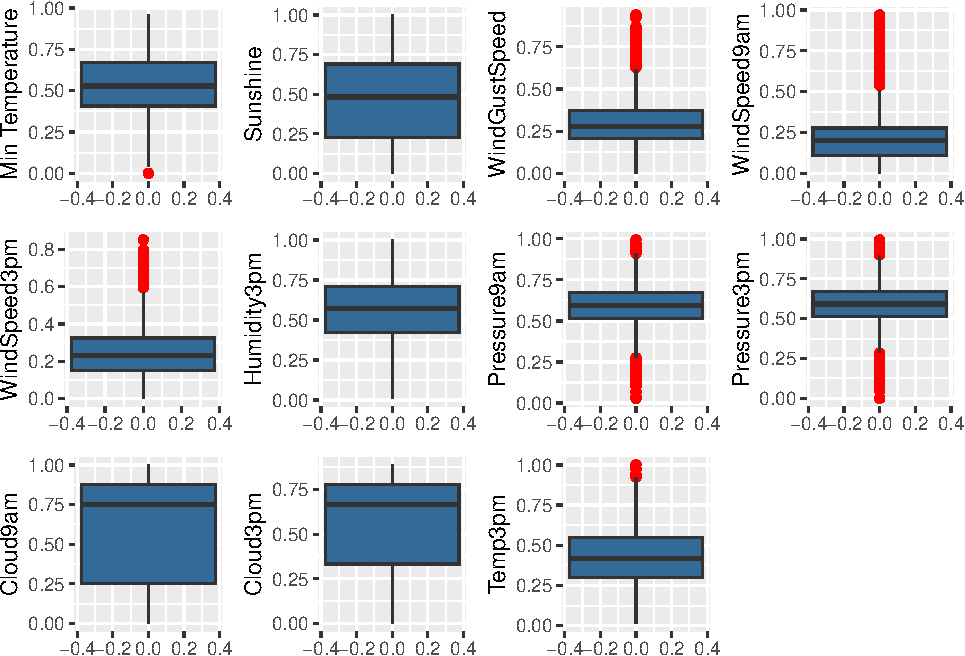
\includegraphics{Rain_Australia_files/figure-latex/Remove outliers-1.pdf}

\begin{Shaded}
\begin{Highlighting}[]
\CommentTok{\#remove outliers for p\_values less that 0.05}
\NormalTok{rain\_subset\_train\_NoOutliers }\OtherTok{\textless{}{-}}\NormalTok{ rain\_subset\_train[}\SpecialCharTok{{-}}\FunctionTok{c}\NormalTok{(}\DecValTok{4596}\NormalTok{,}\DecValTok{10679}\NormalTok{,}\DecValTok{15369}\NormalTok{,}\DecValTok{1935}\NormalTok{,}\DecValTok{3782}\NormalTok{,}
                                                     \DecValTok{10189}\NormalTok{,}\DecValTok{10959}\NormalTok{,}\DecValTok{15362}\NormalTok{,}\DecValTok{16105}\NormalTok{,}
                                                     \DecValTok{18240}\NormalTok{,}\DecValTok{376}\NormalTok{,}\DecValTok{6965}\NormalTok{)]}
\end{Highlighting}
\end{Shaded}

\hypertarget{linear-discriminant-analysis-lda}{%
\subsection{Linear Discriminant Analysis
(LDA)}\label{linear-discriminant-analysis-lda}}

\begin{Shaded}
\begin{Highlighting}[]
\CommentTok{\# Model definition starting from the previous glm\_bal model:}

\NormalTok{lda }\OtherTok{\textless{}{-}}
  \FunctionTok{lda}\NormalTok{(}\AttributeTok{data =}\NormalTok{ rain\_subset\_train\_NoOutliers, RainTomorrow }\SpecialCharTok{\textasciitilde{}}\NormalTok{ ., }\AttributeTok{family =} \StringTok{"binomial"}\NormalTok{)}
\NormalTok{lda}
\end{Highlighting}
\end{Shaded}

\begin{verbatim}
## Call:
## lda(RainTomorrow ~ ., data = rain_subset_train_NoOutliers, family = "binomial")
## 
## Prior probabilities of groups:
##         0         1 
## 0.4986052 0.5013948 
## 
## Group means:
##     MinTemp  Sunshine WindGustSpeed WindSpeed9am WindSpeed3pm Humidity3pm
## 0 0.5198474 0.5981404     0.2639337    0.2044065    0.2354919   0.4472972
## 1 0.5566944 0.3136079     0.3289740    0.2318952    0.2608863   0.6693281
##   Pressure9am Pressure3pm  Cloud9am  Cloud3pm   Temp3pm RainToday
## 0   0.6284978   0.6232747 0.4703169 0.4187170 0.4626215 0.1561222
## 1   0.5583618   0.5622434 0.7413733 0.6944504 0.3922791 0.4574149
## 
## Coefficients of linear discriminants:
##                      LD1
## MinTemp       -0.8224766
## Sunshine      -1.7816536
## WindGustSpeed  3.7461372
## WindSpeed9am  -0.4589668
## WindSpeed3pm  -0.7932450
## Humidity3pm    3.3868009
## Pressure9am    3.5262631
## Pressure3pm   -5.8402214
## Cloud9am      -0.1977520
## Cloud3pm       0.7803935
## Temp3pm        1.3252533
## RainToday      0.3534121
\end{verbatim}

\begin{Shaded}
\begin{Highlighting}[]
\NormalTok{pred\_lda }\OtherTok{\textless{}{-}} \FunctionTok{predict}\NormalTok{(lda, rain\_subset\_test, }\AttributeTok{type =} \StringTok{"response"}\NormalTok{)}

\NormalTok{post\_lda }\OtherTok{\textless{}{-}}\NormalTok{ pred\_lda}\SpecialCharTok{$}\NormalTok{posterior}

\NormalTok{pred\_lda\_04 }\OtherTok{\textless{}{-}} \FunctionTok{as.factor}\NormalTok{(}\FunctionTok{ifelse}\NormalTok{(post\_lda[, }\DecValTok{2}\NormalTok{] }\SpecialCharTok{\textgreater{}}\NormalTok{ threshold4, }\DecValTok{1}\NormalTok{, }\DecValTok{0}\NormalTok{))}
\NormalTok{pred\_lda\_05 }\OtherTok{\textless{}{-}} \FunctionTok{as.factor}\NormalTok{(}\FunctionTok{ifelse}\NormalTok{(post\_lda[, }\DecValTok{2}\NormalTok{] }\SpecialCharTok{\textgreater{}}\NormalTok{ threshold5, }\DecValTok{1}\NormalTok{, }\DecValTok{0}\NormalTok{))}
\NormalTok{pred\_lda\_06 }\OtherTok{\textless{}{-}} \FunctionTok{as.factor}\NormalTok{(}\FunctionTok{ifelse}\NormalTok{(post\_lda[, }\DecValTok{2}\NormalTok{] }\SpecialCharTok{\textgreater{}}\NormalTok{ threshold6, }\DecValTok{1}\NormalTok{, }\DecValTok{0}\NormalTok{))}


\CommentTok{\# Confusion matrix with threshold = 0.4}
\NormalTok{error\_lda4 }\OtherTok{\textless{}{-}} \FunctionTok{mean}\NormalTok{(pred\_lda\_04 }\SpecialCharTok{!=}\NormalTok{ rain\_subset\_test}\SpecialCharTok{$}\NormalTok{RainTomorrow)}
\NormalTok{accuracy\_lda4 }\OtherTok{\textless{}{-}} \FunctionTok{mean}\NormalTok{(pred\_lda\_04 }\SpecialCharTok{==}\NormalTok{ rain\_subset\_test}\SpecialCharTok{$}\NormalTok{RainTomorrow)}
\NormalTok{lda\_CM04 }\OtherTok{\textless{}{-}}
  \FunctionTok{confusionMatrix}\NormalTok{(}
    \AttributeTok{data =} \FunctionTok{factor}\NormalTok{(pred\_lda\_04),}
    \AttributeTok{reference =} \FunctionTok{factor}\NormalTok{(rain\_subset\_test}\SpecialCharTok{$}\NormalTok{RainTomorrow),}
    \AttributeTok{mode =} \StringTok{\textquotesingle{}everything\textquotesingle{}}
\NormalTok{  )}

\CommentTok{\# Confusion matrix with threshold = 0.5}
\NormalTok{error\_lda5 }\OtherTok{\textless{}{-}} \FunctionTok{mean}\NormalTok{(pred\_lda\_05 }\SpecialCharTok{!=}\NormalTok{ rain\_subset\_test}\SpecialCharTok{$}\NormalTok{RainTomorrow)}
\NormalTok{accuracy\_lda5 }\OtherTok{\textless{}{-}} \FunctionTok{mean}\NormalTok{(pred\_lda\_05 }\SpecialCharTok{==}\NormalTok{ rain\_subset\_test}\SpecialCharTok{$}\NormalTok{RainTomorrow)}
\NormalTok{lda\_CM05 }\OtherTok{\textless{}{-}}
  \FunctionTok{confusionMatrix}\NormalTok{(}
    \AttributeTok{data =} \FunctionTok{factor}\NormalTok{(pred\_lda\_05),}
    \AttributeTok{reference =} \FunctionTok{factor}\NormalTok{(rain\_subset\_test}\SpecialCharTok{$}\NormalTok{RainTomorrow),}
    \AttributeTok{mode =} \StringTok{\textquotesingle{}everything\textquotesingle{}}
\NormalTok{  )}

\CommentTok{\# Confusion matrix with threshold = 0.6}
\NormalTok{error\_lda6 }\OtherTok{\textless{}{-}} \FunctionTok{mean}\NormalTok{(pred\_lda\_06 }\SpecialCharTok{!=}\NormalTok{ rain\_subset\_test}\SpecialCharTok{$}\NormalTok{RainTomorrow)}
\NormalTok{accuracy\_lda6 }\OtherTok{\textless{}{-}} \FunctionTok{mean}\NormalTok{(pred\_lda\_06 }\SpecialCharTok{==}\NormalTok{ rain\_subset\_test}\SpecialCharTok{$}\NormalTok{RainTomorrow)}
\NormalTok{lda\_CM06 }\OtherTok{\textless{}{-}}
  \FunctionTok{confusionMatrix}\NormalTok{(}
    \AttributeTok{data =} \FunctionTok{factor}\NormalTok{(pred\_lda\_06),}
    \AttributeTok{reference =} \FunctionTok{factor}\NormalTok{(rain\_subset\_test}\SpecialCharTok{$}\NormalTok{RainTomorrow),}
    \AttributeTok{mode =} \StringTok{\textquotesingle{}everything\textquotesingle{}}
\NormalTok{  )}



\NormalTok{A }\OtherTok{\textless{}{-}}
  \FunctionTok{create\_confusion\_matrix}\NormalTok{(lda\_CM04, }\FloatTok{0.4}\NormalTok{, error\_lda4, accuracy\_lda4)}
\NormalTok{B }\OtherTok{\textless{}{-}}
  \FunctionTok{create\_confusion\_matrix}\NormalTok{(lda\_CM05, }\FloatTok{0.5}\NormalTok{, error\_lda5, accuracy\_lda5)}
\NormalTok{C }\OtherTok{\textless{}{-}}
  \FunctionTok{create\_confusion\_matrix}\NormalTok{(lda\_CM06, }\FloatTok{0.6}\NormalTok{, error\_lda6, accuracy\_lda6)}

\CommentTok{\# Threshold of 0.6 is the best among thresholds in terms of accuracy, }
\CommentTok{\#sensitivity, and specificity}
\NormalTok{CM\_all\_lda }\OtherTok{=} \FunctionTok{list}\NormalTok{(A, B, C)}
\NormalTok{plot\_width }\OtherTok{\textless{}{-}} \FunctionTok{c}\NormalTok{(}\DecValTok{4}\NormalTok{, }\DecValTok{4}\NormalTok{, }\DecValTok{4}\NormalTok{)}
\FunctionTok{grid.arrange}\NormalTok{(}\AttributeTok{grobs =}\NormalTok{ CM\_all\_lda,}
             \AttributeTok{nrow =} \DecValTok{3}\NormalTok{,}
             \AttributeTok{width =}\NormalTok{ plot\_width)}
\end{Highlighting}
\end{Shaded}

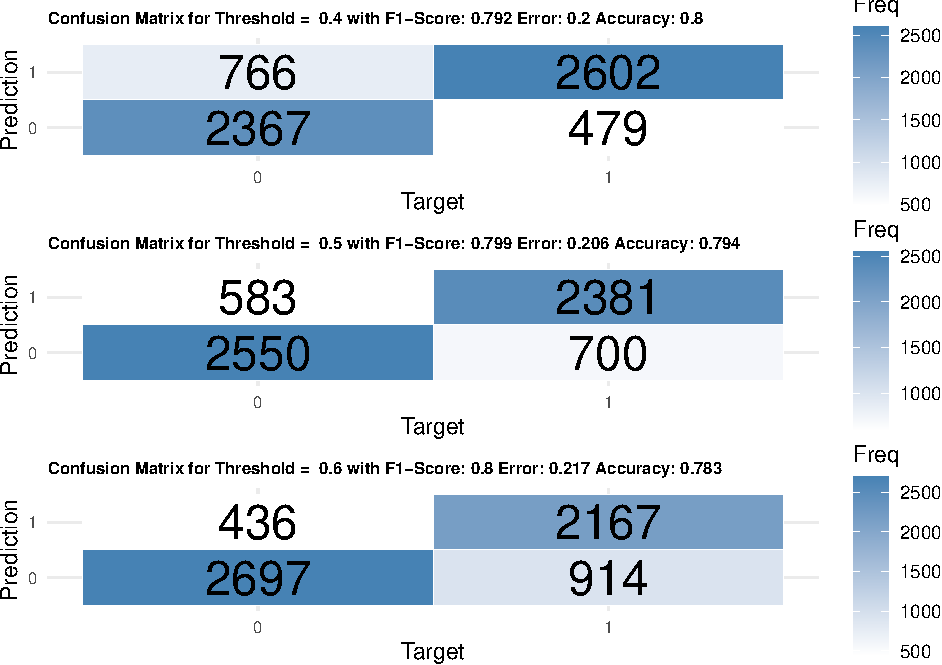
\includegraphics{Rain_Australia_files/figure-latex/LDA-1.pdf}

\begin{Shaded}
\begin{Highlighting}[]
\CommentTok{\# Here we plot stacked histograms representing the linear combination of }
\CommentTok{\# variable that best represent the samples with their discriminant scores, split}
\CommentTok{\#by each assigned class. The y{-}axis is the frequency of examples falling into }
\CommentTok{\# each range of discriminant scores. From these plots, we observed little to no}
\CommentTok{\# overlap across the two classes, which is an indicator of good separation }
\CommentTok{\# between the two classes.}

\FunctionTok{ldahist}\NormalTok{(pred\_lda}\SpecialCharTok{$}\NormalTok{x[, }\DecValTok{1}\NormalTok{], }\AttributeTok{g =}\NormalTok{ pred\_lda}\SpecialCharTok{$}\NormalTok{class, }\AttributeTok{col =} \DecValTok{2}\NormalTok{)}
\end{Highlighting}
\end{Shaded}

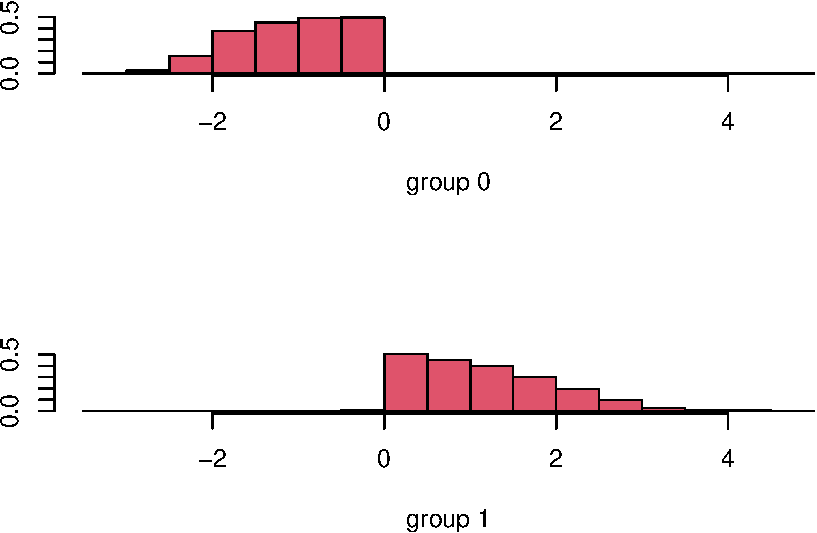
\includegraphics{Rain_Australia_files/figure-latex/LDA histogram-1.pdf}

\hypertarget{quadratic-discriminant-analysis-qda}{%
\subsection{Quadratic Discriminant Analysis
(QDA)}\label{quadratic-discriminant-analysis-qda}}

\begin{Shaded}
\begin{Highlighting}[]
\NormalTok{qda }\OtherTok{\textless{}{-}}
  \FunctionTok{qda}\NormalTok{(}\AttributeTok{data =}\NormalTok{ rain\_subset\_train\_NoOutliers, RainTomorrow }\SpecialCharTok{\textasciitilde{}}\NormalTok{ ., }\AttributeTok{family =} \StringTok{"binomial"}\NormalTok{)}
\NormalTok{qda}
\end{Highlighting}
\end{Shaded}

\begin{verbatim}
## Call:
## qda(RainTomorrow ~ ., data = rain_subset_train_NoOutliers, family = "binomial")
## 
## Prior probabilities of groups:
##         0         1 
## 0.4986052 0.5013948 
## 
## Group means:
##     MinTemp  Sunshine WindGustSpeed WindSpeed9am WindSpeed3pm Humidity3pm
## 0 0.5198474 0.5981404     0.2639337    0.2044065    0.2354919   0.4472972
## 1 0.5566944 0.3136079     0.3289740    0.2318952    0.2608863   0.6693281
##   Pressure9am Pressure3pm  Cloud9am  Cloud3pm   Temp3pm RainToday
## 0   0.6284978   0.6232747 0.4703169 0.4187170 0.4626215 0.1561222
## 1   0.5583618   0.5622434 0.7413733 0.6944504 0.3922791 0.4574149
\end{verbatim}

\begin{Shaded}
\begin{Highlighting}[]
\NormalTok{pred\_qda }\OtherTok{\textless{}{-}} \FunctionTok{predict}\NormalTok{(qda, rain\_subset\_test, }\AttributeTok{type =} \StringTok{"response"}\NormalTok{)}

\NormalTok{post\_qda }\OtherTok{\textless{}{-}}\NormalTok{ pred\_qda}\SpecialCharTok{$}\NormalTok{posterior}

\NormalTok{pred\_qda\_04 }\OtherTok{\textless{}{-}} \FunctionTok{as.factor}\NormalTok{(}\FunctionTok{ifelse}\NormalTok{(post\_qda[, }\DecValTok{2}\NormalTok{] }\SpecialCharTok{\textgreater{}}\NormalTok{ threshold4, }\DecValTok{1}\NormalTok{, }\DecValTok{0}\NormalTok{))}
\NormalTok{pred\_qda\_05 }\OtherTok{\textless{}{-}} \FunctionTok{as.factor}\NormalTok{(}\FunctionTok{ifelse}\NormalTok{(post\_qda[, }\DecValTok{2}\NormalTok{] }\SpecialCharTok{\textgreater{}}\NormalTok{ threshold5, }\DecValTok{1}\NormalTok{, }\DecValTok{0}\NormalTok{))}
\NormalTok{pred\_qda\_06 }\OtherTok{\textless{}{-}} \FunctionTok{as.factor}\NormalTok{(}\FunctionTok{ifelse}\NormalTok{(post\_qda[, }\DecValTok{2}\NormalTok{] }\SpecialCharTok{\textgreater{}}\NormalTok{ threshold6, }\DecValTok{1}\NormalTok{, }\DecValTok{0}\NormalTok{))}


\CommentTok{\# Confusion matrices and performance metrics below indicate very little }
\CommentTok{\#difference across the QDA models with the different thresholds.}

\CommentTok{\# Confusion matrix with threshold = 0.4}
\NormalTok{error\_qda4 }\OtherTok{\textless{}{-}} \FunctionTok{mean}\NormalTok{(pred\_qda\_04 }\SpecialCharTok{!=}\NormalTok{ rain\_subset\_test}\SpecialCharTok{$}\NormalTok{RainTomorrow)}
\NormalTok{accuracy\_qda4 }\OtherTok{\textless{}{-}} \FunctionTok{mean}\NormalTok{(pred\_qda\_04 }\SpecialCharTok{==}\NormalTok{ rain\_subset\_test}\SpecialCharTok{$}\NormalTok{RainTomorrow)}
\NormalTok{qda\_CM04 }\OtherTok{\textless{}{-}}
  \FunctionTok{confusionMatrix}\NormalTok{(}
    \AttributeTok{data =} \FunctionTok{factor}\NormalTok{(pred\_qda\_04),}
    \AttributeTok{reference =} \FunctionTok{factor}\NormalTok{(rain\_subset\_test}\SpecialCharTok{$}\NormalTok{RainTomorrow),}
    \AttributeTok{mode =} \StringTok{\textquotesingle{}everything\textquotesingle{}}
\NormalTok{  )}

\CommentTok{\# Confusion matrix with threshold = 0.5}
\NormalTok{error\_qda5 }\OtherTok{\textless{}{-}} \FunctionTok{mean}\NormalTok{(pred\_qda\_05 }\SpecialCharTok{!=}\NormalTok{ rain\_subset\_test}\SpecialCharTok{$}\NormalTok{RainTomorrow)}
\NormalTok{accuracy\_qda5 }\OtherTok{\textless{}{-}} \FunctionTok{mean}\NormalTok{(pred\_qda\_05 }\SpecialCharTok{==}\NormalTok{ rain\_subset\_test}\SpecialCharTok{$}\NormalTok{RainTomorrow)}
\NormalTok{qda\_CM05 }\OtherTok{\textless{}{-}}
  \FunctionTok{confusionMatrix}\NormalTok{(}
    \AttributeTok{data =} \FunctionTok{factor}\NormalTok{(pred\_qda\_05),}
    \AttributeTok{reference =} \FunctionTok{factor}\NormalTok{(rain\_subset\_test}\SpecialCharTok{$}\NormalTok{RainTomorrow),}
    \AttributeTok{mode =} \StringTok{\textquotesingle{}everything\textquotesingle{}}
\NormalTok{  )}

\CommentTok{\# Confusion matrix with threshold = 0.6}
\NormalTok{error\_qda6 }\OtherTok{\textless{}{-}} \FunctionTok{mean}\NormalTok{(pred\_qda\_06 }\SpecialCharTok{!=}\NormalTok{ rain\_subset\_test}\SpecialCharTok{$}\NormalTok{RainTomorrow)}
\NormalTok{accuracy\_qda6 }\OtherTok{\textless{}{-}} \FunctionTok{mean}\NormalTok{(pred\_qda\_06 }\SpecialCharTok{==}\NormalTok{ rain\_subset\_test}\SpecialCharTok{$}\NormalTok{RainTomorrow)}
\NormalTok{qda\_CM06 }\OtherTok{\textless{}{-}}
  \FunctionTok{confusionMatrix}\NormalTok{(}
    \AttributeTok{data =} \FunctionTok{factor}\NormalTok{(pred\_qda\_06),}
    \AttributeTok{reference =} \FunctionTok{factor}\NormalTok{(rain\_subset\_test}\SpecialCharTok{$}\NormalTok{RainTomorrow),}
    \AttributeTok{mode =} \StringTok{\textquotesingle{}everything\textquotesingle{}}
\NormalTok{  )}

\NormalTok{A }\OtherTok{\textless{}{-}}
  \FunctionTok{create\_confusion\_matrix}\NormalTok{(qda\_CM04, }\FloatTok{0.4}\NormalTok{, error\_qda4, accuracy\_qda4)}
\NormalTok{B }\OtherTok{\textless{}{-}}
  \FunctionTok{create\_confusion\_matrix}\NormalTok{(qda\_CM05, }\FloatTok{0.5}\NormalTok{, error\_qda5, accuracy\_qda5)}
\NormalTok{C }\OtherTok{\textless{}{-}}
  \FunctionTok{create\_confusion\_matrix}\NormalTok{(qda\_CM06, }\FloatTok{0.6}\NormalTok{, error\_qda6, accuracy\_qda6)}

\CommentTok{\# Threshold of 0.05 is the best among thresholds in terms of accuracy, }
\CommentTok{\# sensitivity, and specificity}
\NormalTok{CM\_all\_qda }\OtherTok{=} \FunctionTok{list}\NormalTok{(A, B, C)}
\NormalTok{plot\_width }\OtherTok{\textless{}{-}} \FunctionTok{c}\NormalTok{(}\DecValTok{4}\NormalTok{, }\DecValTok{4}\NormalTok{, }\DecValTok{4}\NormalTok{)}
\FunctionTok{grid.arrange}\NormalTok{(}\AttributeTok{grobs =}\NormalTok{ CM\_all\_qda,}
             \AttributeTok{nrow =} \DecValTok{3}\NormalTok{,}
             \AttributeTok{width =}\NormalTok{ plot\_width)}
\end{Highlighting}
\end{Shaded}

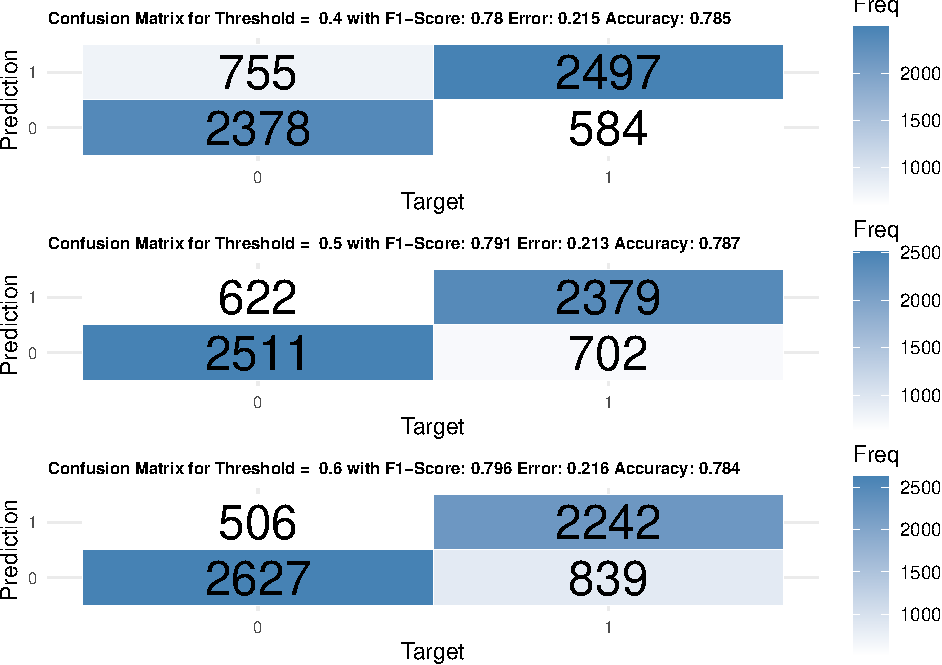
\includegraphics{Rain_Australia_files/figure-latex/QDA-1.pdf}

\hypertarget{k-nearest-neighbors-knn}{%
\section{K-Nearest Neighbors (kNN)}\label{k-nearest-neighbors-knn}}

K-Nearest Neighbors (KNN) is a non-parametric, supervised learning
technique, which assumes that features that are close in the feature
space belong to the same class. The model identifies the labeled
K-closest points to an observed point, and assigns the point to the
majority class of the said-K-nearest neighbors. KNN is very sensitive to
feature scaling and choice of K. If K is too small, KNN might lead to
overfitting as each point is classified according to a small set of
training examples. Choosing a K that is too large, however, may lead to
less overfitting, but with the tradeoff of higher bias and too simple of
a model.

\begin{Shaded}
\begin{Highlighting}[]
\FunctionTok{set.seed}\NormalTok{(}\DecValTok{2531}\NormalTok{)}

\CommentTok{\# We look now for the best value of the parameter}
\NormalTok{kmax }\OtherTok{\textless{}{-}} \DecValTok{100}
\NormalTok{knn\_test\_error }\OtherTok{\textless{}{-}} \FunctionTok{numeric}\NormalTok{(kmax)}

\CommentTok{\# For each possible value of k we consider the obtained accuracy of the model}
\ControlFlowTok{for}\NormalTok{ (k }\ControlFlowTok{in} \DecValTok{1}\SpecialCharTok{:}\NormalTok{kmax)}
\NormalTok{\{}
\NormalTok{  knn\_pred }\OtherTok{\textless{}{-}}
    \FunctionTok{as.factor}\NormalTok{(}\FunctionTok{knn}\NormalTok{(X\_train\_subset, X\_test\_subset, }\AttributeTok{cl =}\NormalTok{ y\_train\_subset, }\AttributeTok{k =}\NormalTok{ k))}
  
\NormalTok{  cm }\OtherTok{\textless{}{-}} \FunctionTok{confusionMatrix}\NormalTok{(}\AttributeTok{data =}\NormalTok{ knn\_pred, }\AttributeTok{reference =}\NormalTok{ y\_test\_subset)}
  
\NormalTok{  knn\_test\_error[k] }\OtherTok{\textless{}{-}} \DecValTok{1} \SpecialCharTok{{-}}\NormalTok{ cm}\SpecialCharTok{$}\NormalTok{overall[}\DecValTok{1}\NormalTok{]}
\NormalTok{\}}

\CommentTok{\# We took the minimum value of the error}
\NormalTok{k\_min }\OtherTok{\textless{}{-}} \FunctionTok{which.min}\NormalTok{(knn\_test\_error)}
\NormalTok{k\_min}
\end{Highlighting}
\end{Shaded}

\begin{verbatim}
## [1] 29
\end{verbatim}

\begin{Shaded}
\begin{Highlighting}[]
\CommentTok{\# We compute now the prediction with the value of k that gives us the minimum error}
\NormalTok{knn }\OtherTok{\textless{}{-}}
  \FunctionTok{knn}\NormalTok{(X\_train\_subset, X\_test\_subset, }\AttributeTok{cl =}\NormalTok{ y\_train\_subset, }\AttributeTok{k =}\NormalTok{ k\_min)}

\NormalTok{knn\_pred\_min }\OtherTok{\textless{}{-}}\NormalTok{ knn}

\CommentTok{\# Confusion matrix for KNN on the test set}
\NormalTok{cm\_knn }\OtherTok{\textless{}{-}}
  \FunctionTok{confusionMatrix}\NormalTok{(}\AttributeTok{data =}\NormalTok{ knn\_pred\_min ,}
                  \AttributeTok{reference =}\NormalTok{ rain\_subset\_test}\SpecialCharTok{$}\NormalTok{RainTomorrow,}
                  \AttributeTok{mode =} \StringTok{\textquotesingle{}everything\textquotesingle{}}\NormalTok{)}

\NormalTok{cm\_table\_knn }\OtherTok{\textless{}{-}} \FunctionTok{as.data.frame}\NormalTok{(cm\_knn}\SpecialCharTok{$}\NormalTok{table)}

\NormalTok{f1\_score\_knn }\OtherTok{\textless{}{-}}\NormalTok{ cm\_knn}\SpecialCharTok{$}\NormalTok{byClass[}\StringTok{"F1"}\NormalTok{]}
\NormalTok{error\_knn }\OtherTok{\textless{}{-}} \FunctionTok{mean}\NormalTok{(knn\_pred\_min }\SpecialCharTok{!=}\NormalTok{ rain\_subset\_test}\SpecialCharTok{$}\NormalTok{RainTomorrow)}
\NormalTok{accuracy\_knn }\OtherTok{\textless{}{-}} \FunctionTok{mean}\NormalTok{(knn\_pred\_min }\SpecialCharTok{==}\NormalTok{ rain\_subset\_test}\SpecialCharTok{$}\NormalTok{RainTomorrow)}

\FunctionTok{ggplot}\NormalTok{(}\AttributeTok{data =}\NormalTok{ cm\_table\_knn, }\FunctionTok{aes}\NormalTok{(}\AttributeTok{x =}\NormalTok{ Reference, }\AttributeTok{y =}\NormalTok{ Prediction, }\AttributeTok{fill =}\NormalTok{ Freq)) }\SpecialCharTok{+}
  \FunctionTok{geom\_tile}\NormalTok{(}\AttributeTok{color =} \StringTok{"white"}\NormalTok{) }\SpecialCharTok{+}
  \FunctionTok{geom\_text}\NormalTok{(}\FunctionTok{aes}\NormalTok{(}\AttributeTok{label =}\NormalTok{ Freq), }\AttributeTok{color =} \StringTok{"black"}\NormalTok{, }\AttributeTok{size =} \DecValTok{8}\NormalTok{) }\SpecialCharTok{+}
  \FunctionTok{scale\_fill\_gradient}\NormalTok{(}\AttributeTok{low =} \StringTok{"white"}\NormalTok{, }\AttributeTok{high =} \StringTok{"steelblue"}\NormalTok{) }\SpecialCharTok{+}
  \FunctionTok{labs}\NormalTok{(}
    \AttributeTok{title =} \FunctionTok{paste}\NormalTok{(}
      \StringTok{"Confusion Matrix for KNN with F1{-}Score:"}\NormalTok{,}
      \FunctionTok{round}\NormalTok{(f1\_score\_knn, }\DecValTok{3}\NormalTok{),}
      \StringTok{"Error:"}\NormalTok{,}
      \FunctionTok{round}\NormalTok{(error\_knn, }\DecValTok{3}\NormalTok{) ,}
      \StringTok{"Accuracy:"}\NormalTok{,}
      \FunctionTok{round}\NormalTok{(accuracy\_knn, }\DecValTok{3}\NormalTok{)}
\NormalTok{    ),}
    \AttributeTok{x =} \StringTok{"Target"}\NormalTok{,}
    \AttributeTok{y =} \StringTok{"Prediction"}
\NormalTok{  ) }\SpecialCharTok{+}
  \FunctionTok{theme\_minimal}\NormalTok{() }\SpecialCharTok{+}
  \FunctionTok{theme}\NormalTok{(}\AttributeTok{axis.text =} \FunctionTok{element\_text}\NormalTok{(}\AttributeTok{size =} \DecValTok{8}\NormalTok{),}
        \AttributeTok{plot.title =} \FunctionTok{element\_text}\NormalTok{(}\AttributeTok{size =} \DecValTok{8}\NormalTok{, }\AttributeTok{face =} \StringTok{"bold"}\NormalTok{))}
\end{Highlighting}
\end{Shaded}

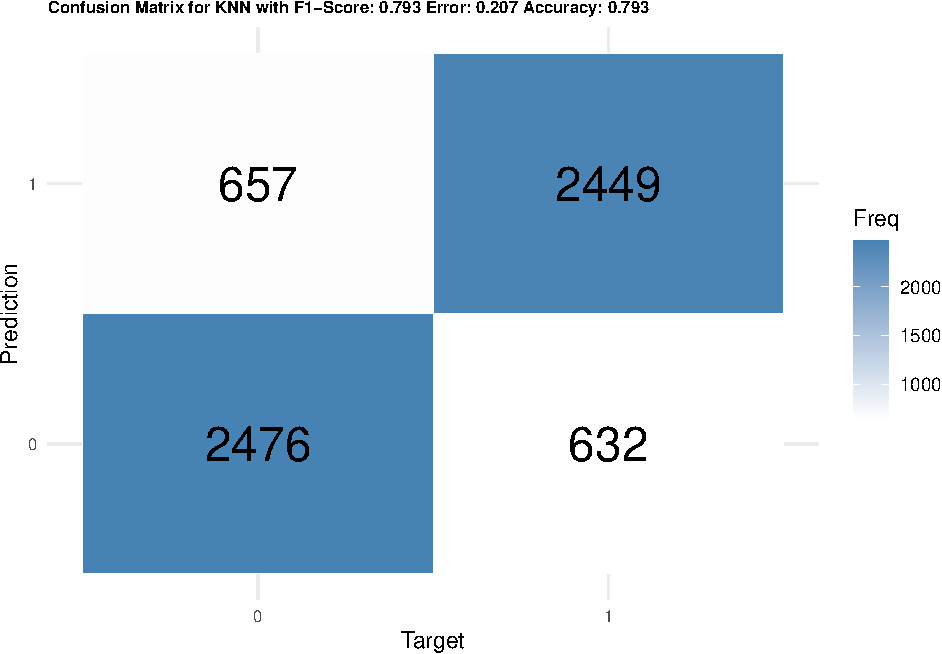
\includegraphics{Rain_Australia_files/figure-latex/KNN-1.pdf}

\begin{Shaded}
\begin{Highlighting}[]
\CommentTok{\#Plot test error against different levels of K}
\FunctionTok{ggplot}\NormalTok{(}\FunctionTok{data.frame}\NormalTok{(knn\_test\_error), }
      \FunctionTok{aes}\NormalTok{(}\AttributeTok{x =} \DecValTok{1}\SpecialCharTok{:}\NormalTok{kmax, }\AttributeTok{y =}\NormalTok{ knn\_test\_error)) }\SpecialCharTok{+}
      \FunctionTok{geom\_line}\NormalTok{(}\AttributeTok{colour=}\StringTok{"blue"}\NormalTok{) }\SpecialCharTok{+}
      \FunctionTok{geom\_point}\NormalTok{(}\AttributeTok{colour=}\StringTok{"red"}\NormalTok{) }\SpecialCharTok{+}
      \FunctionTok{xlab}\NormalTok{(}\StringTok{"K (\#neighbors)"}\NormalTok{) }\SpecialCharTok{+} 
      \FunctionTok{ylab}\NormalTok{(}\StringTok{"Test error"}\NormalTok{) }\SpecialCharTok{+}
      \FunctionTok{ggtitle}\NormalTok{(}\FunctionTok{paste0}\NormalTok{(}\StringTok{"Best value of K = "}\NormalTok{, k\_min,}
                     \StringTok{" (minimal error = "}\NormalTok{,}
                    \FunctionTok{format}\NormalTok{((knn\_test\_error[k\_min])}\SpecialCharTok{*}\DecValTok{100}\NormalTok{, }\AttributeTok{digits =} \DecValTok{4}\NormalTok{), }
                    \StringTok{"\%)"}\NormalTok{))}
\end{Highlighting}
\end{Shaded}

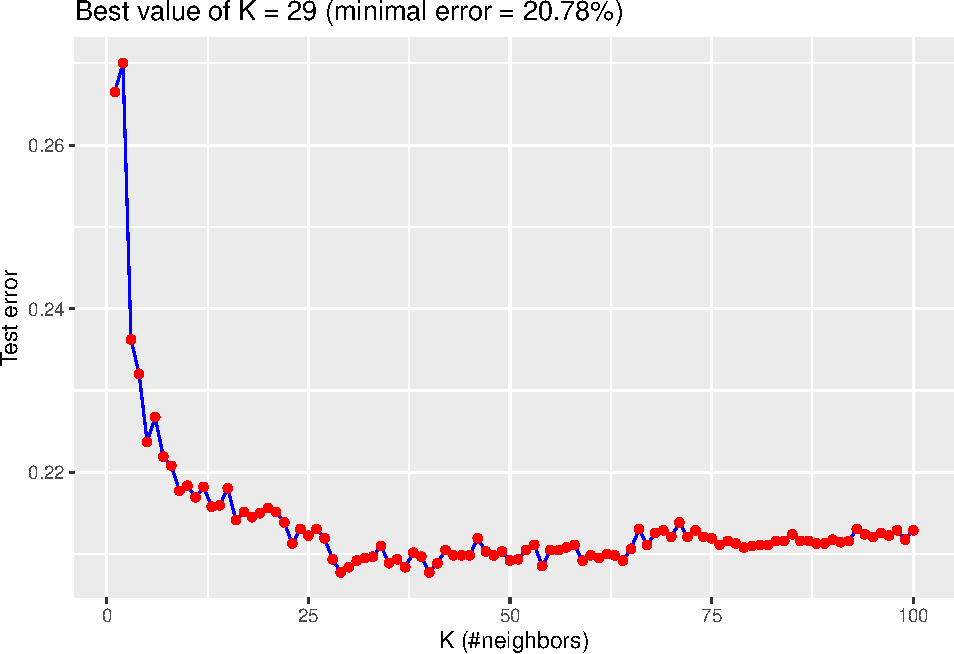
\includegraphics{Rain_Australia_files/figure-latex/plot error-1.pdf}

\hypertarget{roc-curves}{%
\section{ROC Curves}\label{roc-curves}}

In this final section, we are going to compare all the models applied to
balanced and subsetted data and generate a ROC curve to plot the False
Positive rate (x-axis) against the True Positive rate (y-axis). This
ultimately allows us to visualize the specificity, deduced from the
false positives (1-false positive = specificity), and sensitivity from
the true positives of each model and between models. We excluded KNN
from this analysis, since we are unable to analyze thresholds for
predicting classes since the model generates strict 0/1 classifications.

\begin{Shaded}
\begin{Highlighting}[]
\CommentTok{\# Best Models:}

\FunctionTok{set.seed}\NormalTok{(}\DecValTok{125}\NormalTok{)}

\CommentTok{\# GLM Model}
\NormalTok{best\_glm\_model }\OtherTok{\textless{}{-}}\NormalTok{ glm\_model}

\NormalTok{best\_glm\_predict }\OtherTok{\textless{}{-}}\NormalTok{ glm\_predict}

\CommentTok{\# LDA Model}
\NormalTok{best\_lda\_model }\OtherTok{\textless{}{-}}
  \FunctionTok{lda}\NormalTok{(}\AttributeTok{data =}\NormalTok{ rain\_subset\_train, RainTomorrow }\SpecialCharTok{\textasciitilde{}}\NormalTok{ ., }\AttributeTok{family =} \StringTok{"binomial"}\NormalTok{)}

\NormalTok{best\_lda\_predict }\OtherTok{\textless{}{-}}
  \FunctionTok{predict}\NormalTok{(lda, rain\_subset\_test, }\AttributeTok{type =} \StringTok{"response"}\NormalTok{)}
\NormalTok{best\_post\_lda }\OtherTok{\textless{}{-}}\NormalTok{ best\_lda\_predict}\SpecialCharTok{$}\NormalTok{posterior}

\CommentTok{\# QDA Model}
\NormalTok{best\_qda\_model }\OtherTok{\textless{}{-}}
  \FunctionTok{qda}\NormalTok{(}\AttributeTok{data =}\NormalTok{ rain\_subset\_train, RainTomorrow }\SpecialCharTok{\textasciitilde{}}\NormalTok{ ., }\AttributeTok{family =} \StringTok{"binomial"}\NormalTok{)}

\NormalTok{best\_qda\_predict }\OtherTok{\textless{}{-}}
  \FunctionTok{predict}\NormalTok{(qda, rain\_subset\_test, }\AttributeTok{type =} \StringTok{"response"}\NormalTok{)}
\NormalTok{best\_post\_qda }\OtherTok{\textless{}{-}}\NormalTok{ best\_qda\_predict}\SpecialCharTok{$}\NormalTok{posterior}

\CommentTok{\# LASSO Model}
\NormalTok{best\_lasso\_model }\OtherTok{\textless{}{-}}\NormalTok{ lasso\_cv\_subset}

\NormalTok{best\_lasso\_predict }\OtherTok{\textless{}{-}}\NormalTok{ pred\_lasso\_subset}

\CommentTok{\# Ridge Model}
\NormalTok{best\_ridge\_model }\OtherTok{\textless{}{-}}\NormalTok{ ridge\_cv\_subset}

\NormalTok{best\_ridge\_predict }\OtherTok{\textless{}{-}}\NormalTok{ pred\_ridge\_subset}

\NormalTok{prediction }\OtherTok{\textless{}{-}}
  \FunctionTok{tibble}\NormalTok{(}\AttributeTok{truth =} \FunctionTok{as.factor}\NormalTok{(rain\_subset\_test}\SpecialCharTok{$}\NormalTok{RainTomorrow))}
\NormalTok{prediction }\OtherTok{\textless{}{-}}
\NormalTok{  prediction }\SpecialCharTok{\%\textgreater{}\%} \FunctionTok{mutate}\NormalTok{(}\AttributeTok{pred =} \FunctionTok{as.numeric}\NormalTok{(best\_glm\_predict)) }\SpecialCharTok{\%\textgreater{}\%} 
  \FunctionTok{mutate}\NormalTok{(}\AttributeTok{model =} \StringTok{"GLM"}\NormalTok{) }\SpecialCharTok{\%\textgreater{}\%}
  \FunctionTok{add\_row}\NormalTok{(}
    \AttributeTok{truth =} \FunctionTok{as.factor}\NormalTok{(rain\_subset\_test}\SpecialCharTok{$}\NormalTok{RainTomorrow),}
    \AttributeTok{pred =} \FunctionTok{as.numeric}\NormalTok{(best\_post\_lda[, }\DecValTok{2}\NormalTok{]),}
    \AttributeTok{model =} \StringTok{"LDA"}
\NormalTok{  ) }\SpecialCharTok{\%\textgreater{}\%}
  \FunctionTok{add\_row}\NormalTok{(}
    \AttributeTok{truth =} \FunctionTok{as.factor}\NormalTok{(rain\_subset\_test}\SpecialCharTok{$}\NormalTok{RainTomorrow),}
    \AttributeTok{pred =} \FunctionTok{as.numeric}\NormalTok{(best\_post\_qda[, }\DecValTok{2}\NormalTok{]),}
    \AttributeTok{model =} \StringTok{"QDA"}
\NormalTok{  ) }\SpecialCharTok{\%\textgreater{}\%}
  \FunctionTok{add\_row}\NormalTok{(}
    \AttributeTok{truth =} \FunctionTok{as.factor}\NormalTok{(rain\_subset\_test}\SpecialCharTok{$}\NormalTok{RainTomorrow),}
    \AttributeTok{pred =} \FunctionTok{as.numeric}\NormalTok{(best\_ridge\_predict),}
    \AttributeTok{model =} \StringTok{"Ridge"}
\NormalTok{  ) }\SpecialCharTok{\%\textgreater{}\%}
  \FunctionTok{add\_row}\NormalTok{(}
    \AttributeTok{truth =} \FunctionTok{as.factor}\NormalTok{(rain\_subset\_test}\SpecialCharTok{$}\NormalTok{RainTomorrow),}
    \AttributeTok{pred =} \FunctionTok{as.numeric}\NormalTok{(best\_lasso\_predict),}
    \AttributeTok{model =} \StringTok{"Lasso"}
\NormalTok{  )}

\CommentTok{\# Calculate ROC curves for each model}
\NormalTok{roc\_list }\OtherTok{\textless{}{-}}
  \FunctionTok{lapply}\NormalTok{(}\FunctionTok{split}\NormalTok{(prediction, prediction}\SpecialCharTok{$}\NormalTok{model), }\ControlFlowTok{function}\NormalTok{(df) \{}
\NormalTok{    roc.out }\OtherTok{\textless{}{-}} \FunctionTok{roc}\NormalTok{(df}\SpecialCharTok{$}\NormalTok{truth, df}\SpecialCharTok{$}\NormalTok{pred, }\AttributeTok{levels =} \FunctionTok{c}\NormalTok{(}\DecValTok{0}\NormalTok{, }\DecValTok{1}\NormalTok{))}
\NormalTok{    roc.df }\OtherTok{\textless{}{-}} \FunctionTok{data.frame}\NormalTok{(}\AttributeTok{specificity =}\NormalTok{ roc.out}\SpecialCharTok{$}\NormalTok{specificities,}
                         \AttributeTok{sensitivity =}\NormalTok{ roc.out}\SpecialCharTok{$}\NormalTok{sensitivities)}
    \FunctionTok{return}\NormalTok{(roc.df)}
\NormalTok{  \})}

\NormalTok{model\_colors }\OtherTok{\textless{}{-}} \FunctionTok{c}\NormalTok{(}\StringTok{"red"}\NormalTok{, }\StringTok{"blue"}\NormalTok{, }\StringTok{"green"}\NormalTok{, }\StringTok{"orange"}\NormalTok{, }\StringTok{"black"}\NormalTok{)}
\CommentTok{\#List of Model Names}
\NormalTok{model\_names }\OtherTok{\textless{}{-}} \FunctionTok{names}\NormalTok{(roc\_list)}

\FunctionTok{ggplot}\NormalTok{() }\SpecialCharTok{+}
  \FunctionTok{lapply}\NormalTok{(}\FunctionTok{seq\_along}\NormalTok{(roc\_list), }\ControlFlowTok{function}\NormalTok{(i) \{}
    \FunctionTok{geom\_line}\NormalTok{(}
      \AttributeTok{data =}\NormalTok{ roc\_list[[i]],}
      \FunctionTok{aes}\NormalTok{(}
        \AttributeTok{x =} \DecValTok{1} \SpecialCharTok{{-}}\NormalTok{ specificity,}
        \AttributeTok{y =}\NormalTok{ sensitivity,}
        \AttributeTok{color =}\NormalTok{ model\_colors[i]}
\NormalTok{      ),}
      \AttributeTok{linetype =} \StringTok{"solid"}\NormalTok{,}
      \AttributeTok{linewidth =} \FloatTok{0.7}
\NormalTok{    )}
\NormalTok{  \}) }\SpecialCharTok{+}
  \FunctionTok{lapply}\NormalTok{(}\FunctionTok{seq\_along}\NormalTok{(roc\_list), }\ControlFlowTok{function}\NormalTok{(i) \{}
    \FunctionTok{labs}\NormalTok{(}
      \AttributeTok{title =} \StringTok{"ROC Curves"}\NormalTok{,}
      \AttributeTok{x =} \StringTok{"False Positive Rate"}\NormalTok{,}
      \AttributeTok{y =} \StringTok{"True Positive Rate"}\NormalTok{,}
      \AttributeTok{color =} \StringTok{"Models"}
\NormalTok{    )}
\NormalTok{  \}) }\SpecialCharTok{+}
  \FunctionTok{scale\_color\_manual}\NormalTok{(}\AttributeTok{values =}\NormalTok{ model\_colors, }\AttributeTok{labels =}\NormalTok{ model\_names) }\SpecialCharTok{+}
  \FunctionTok{theme\_minimal}\NormalTok{() }
\end{Highlighting}
\end{Shaded}

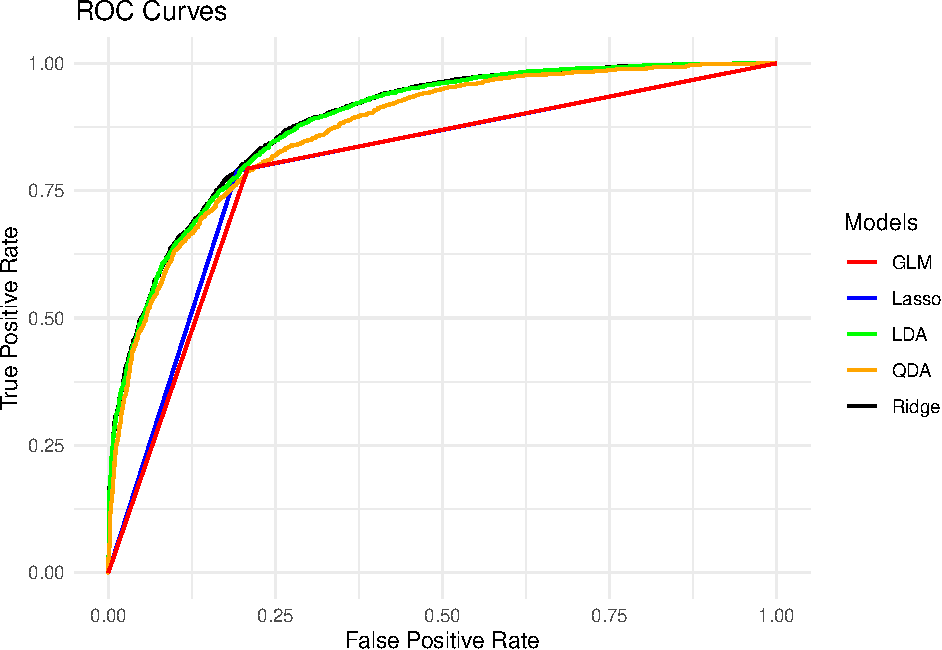
\includegraphics{Rain_Australia_files/figure-latex/ROC-1.pdf}

\hypertarget{discussion}{%
\section{Discussion}\label{discussion}}

The area under each of the ROC curves for each model serves as an
indicator for how well each model predicts RainTomorrow.The larger the
area under the curve (AUC), the higher the recall of the model is
(positivity rate). We can observe that the ridge, LDA, and QDA show a
better AUC compared to GLM and LASSO models. In some cases concerning
fatalities or hazardous situations, we care more about achieving a
tradeoff between false positives and true positives in order to minimize
false negatives. Thus, the ROC curves are suitable for modeling these
cases. However, in our case, we care more generally about a model that
predicts well than having this tradeoff between false positives and true
positives. On the other hand, other projects using this data may give
higher consideration to positive rain predictions, such as projects in
the agriculture sector, where having rain tomorrow may impact the
harvest season. To address our concern with prioritizing more precise
predictions over the positivity rate, we extended our final analysis of
the models by considering the key performance metrics, i.e. F1 Score,
accuracy, error rate, for each model.

\begin{Shaded}
\begin{Highlighting}[]
\NormalTok{file\_path3 }\OtherTok{\textless{}{-}} \StringTok{"/Users/Sofia/Desktop/Rain\_Australia/metrics\_summary.csv"}
\NormalTok{metrics\_summary }\OtherTok{\textless{}{-}} \FunctionTok{read.csv}\NormalTok{(file\_path3)}

\FunctionTok{options}\NormalTok{(}\AttributeTok{knitr.kable.NA =} \StringTok{\textquotesingle{}\textquotesingle{}}\NormalTok{)}
\NormalTok{metrics\_summary }\SpecialCharTok{\%\textgreater{}\%}
\NormalTok{  knitr}\SpecialCharTok{::}\FunctionTok{kable}\NormalTok{(}
    \AttributeTok{format =} \StringTok{"latex"}\NormalTok{,}
    \AttributeTok{align =} \StringTok{"l"}\NormalTok{,}
    \AttributeTok{booktabs =} \ConstantTok{TRUE}\NormalTok{,}
    \AttributeTok{longtable =} \ConstantTok{TRUE}\NormalTok{,}
    \AttributeTok{linesep =} \StringTok{""}\NormalTok{,}
    \AttributeTok{caption =} \StringTok{"Table of performance metrics by model."}
\NormalTok{    ) }\SpecialCharTok{\%\textgreater{}\%} \FunctionTok{row\_spec}\NormalTok{(}\DecValTok{0}\NormalTok{,}\AttributeTok{bold=}\ConstantTok{TRUE}\NormalTok{) }\SpecialCharTok{\%\textgreater{}\%} 
\NormalTok{  kableExtra}\SpecialCharTok{::}\FunctionTok{kable\_styling}\NormalTok{(}
      \AttributeTok{position =} \StringTok{"left"}\NormalTok{,}
      \AttributeTok{latex\_options =} \FunctionTok{c}\NormalTok{(}\StringTok{"striped"}\NormalTok{, }\StringTok{"repeat\_header"}\NormalTok{),}
      \AttributeTok{stripe\_color =} \StringTok{"gray!15"}
\NormalTok{    )}
\end{Highlighting}
\end{Shaded}

\begin{longtable}[l]{llll}
\caption{\label{tab:Final Model Comparisons}Table of performance metrics by model.}\\
\toprule
\textbf{Model} & \textbf{F1.Score} & \textbf{Error} & \textbf{Accuracy}\\
\midrule
\endfirsthead
\caption[]{Table of performance metrics by model. \textit{(continued)}}\\
\toprule
\textbf{Model} & \textbf{F1.Score} & \textbf{Error} & \textbf{Accuracy}\\
\midrule
\endhead

\endfoot
\bottomrule
\endlastfoot
\cellcolor{gray!15}{Simple GLM 0.4} & \cellcolor{gray!15}{0.903} & \cellcolor{gray!15}{0.153} & \cellcolor{gray!15}{0.847}\\
Simple GLM 0.5 & 0.907 & 0.149 & 0.851\\
\cellcolor{gray!15}{Simple GLM 0.6} & \cellcolor{gray!15}{0.907} & \cellcolor{gray!15}{0.153} & \cellcolor{gray!15}{0.847}\\
 &  &  \vphantom{6} & \\
\cellcolor{gray!15}{GLM with Balanced Dataset-0.4} & \cellcolor{gray!15}{0.781} & \cellcolor{gray!15}{0.205} & \cellcolor{gray!15}{0.795}\\
GLM with Balanced Dataset-0.5 & 0.796 & 0.205 & 0.795\\
\cellcolor{gray!15}{GLM with Balanced Dataset-0.6} & \cellcolor{gray!15}{0.798} & \cellcolor{gray!15}{0.215} & \cellcolor{gray!15}{0.785}\\
 &  &  \vphantom{5} & \\
\cellcolor{gray!15}{GLM with balancing and feature selection-0.4} & \cellcolor{gray!15}{0.781} & \cellcolor{gray!15}{0.206} & \cellcolor{gray!15}{0.794}\\
GLM with balancing and feature selection-0.5 & 0.795 & 0.205 & 0.795\\
\cellcolor{gray!15}{GLM with balancing and feature selection-0.6} & \cellcolor{gray!15}{0.797} & \cellcolor{gray!15}{0.216} & \cellcolor{gray!15}{0.784}\\
 &  &  \vphantom{4} & \\
\cellcolor{gray!15}{LDA with balancing and feature seletion-0.4} & \cellcolor{gray!15}{0.783} & \cellcolor{gray!15}{0.207} & \cellcolor{gray!15}{0.793}\\
LDA with balancing and feature seletion-0.5 & 0.792 & 0.210 & 0.790\\
\cellcolor{gray!15}{LDA with balancing and feature seletion-0.6} & \cellcolor{gray!15}{0.795} & \cellcolor{gray!15}{0.220} & \cellcolor{gray!15}{0.780}\\
 &  &  \vphantom{3} & \\
\cellcolor{gray!15}{QDA with balancing and feature seletion-0.4} & \cellcolor{gray!15}{0.776} & \cellcolor{gray!15}{0.217} & \cellcolor{gray!15}{0.783}\\
QDA with balancing and feature seletion-0.5 & 0.785 & 0.216 & 0.784\\
\cellcolor{gray!15}{QDA with balancing and feature seletion-0.6} & \cellcolor{gray!15}{0.788} & \cellcolor{gray!15}{0.220} & \cellcolor{gray!15}{0.780}\\
 &  &  \vphantom{2} & \\
\cellcolor{gray!15}{Ridge Regression with balancing} & \cellcolor{gray!15}{0.786} & \cellcolor{gray!15}{0.213} & \cellcolor{gray!15}{0.787}\\
Ridge Regression with balancing and feature selection & 0.786 & 0.213 & 0.787\\
\cellcolor{gray!15}{} & \cellcolor{gray!15}{} & \cellcolor{gray!15}{ \vphantom{1}} & \cellcolor{gray!15}{}\\
Lasso Regression with balancing & 0.796 & 0.205 & 0.795\\
\cellcolor{gray!15}{Lasso Regression with balancing and feature selection} & \cellcolor{gray!15}{0.794} & \cellcolor{gray!15}{0.206} & \cellcolor{gray!15}{0.794}\\
 &  &  & \\
\cellcolor{gray!15}{KNN} & \cellcolor{gray!15}{0.782} & \cellcolor{gray!15}{0.216} & \cellcolor{gray!15}{0.784}\\*
\end{longtable}

While in the ROC curves, Ridge, LDA and QDA performed better, the GLM
models had the best performance metrics overall. These results suggest
that compared to other models, the logistic regression model is the most
precise in predicting RainTomorrow.

\end{document}
